%% Latex template for PhD dissertation or MS thesis
%% Department of Mechanical Engineering
%% Brigham Young University
%% Last Modified: April 2017

% \documentclass[12pt,twoside]{report}% Use this line for the print version of the thesis
\documentclass[12pt,oneside]{report}% If you comment out the line above, and uncomment this line, it will create a file without the extra pages that the Library wants for its electronic file versions.

%%%%%%%%%%%%%%%%%%%%%%%%%%%%%%%%%%%%%%%%%%%%%%%%%%%%%%%%%
%  Setup BYU thesis format
%%%%%%%%%%%%%%%%%%%%%%%%%%%%%%%%%%%%%%%%%%%%%%%%%%%%%%%%%
\usepackage{byustyle}
% Setup the byu style sheet
\byustylesetup{%
    %
    %isdissertation = true,            % Uncomment this if you're doing a PhD dissertation
    %
    % Definitions of names needed in thesis/dissertation
    deptname          = Department of Mechanical Engineering,
    committeechairman = Timothy W. McLain,
    committeemembera  = Randal W. Beard,
    committeememberb  = Marc D. Killpack,
    graddate = December 2019,  		% Final approval month (NOT graduation month!        	
     %
    %Uncomment to shorten for proofreading purposes
    %noabstract = true,         % Don't show the abstract page
    %nouniversitypages = true,  % Don't show any of the "university pages"
    %noacknowledgements = true, % Don't show the Acknowledgements page
    %notableofcontents = true,  % Don't show the Table of Contents
    %nolistoffigures = true,    % Don't show the List of Figures
   % nolistoftables = true,     % Don't show the List of Tables
    nonomenclature = true,     % Don't show the Nomenclature section - note that this section is optional
    %notocandlists = true,      % Don't show the Table of Contents, List of Figures, or the List of Tables
    % noheaderatall = true,      % Don't show any of the BYU Thesis header pages
    keywords = {state estimation, optimal control, unmanned vehicles, autonomous vehicles, error state, multirotor, micro air vehicle,
      linear quadratic regulator, LQR, UAV} % Enter your keywords
%inside the curly braces, as you'd like them to appear on the bottom of the abstract page.
}
%%%%%%%%%%%%%%%%%%%%%%%%%%%%%%%%%%%%%%%%%%%%%%%%%%%%%%%%
%  Include other \usepackage{} statements here.
%    Add one package at a time.
%    Warning:  Some packages are not compatible with byuthesis.sty
%%%%%%%%%%%%%%%%%%%%%%%%%%%%%%%%%%%%%%%%%%%%%%%%%%%%%%%%%
% You should turn on any of these that you think you'll need!
%\usepackage[normalmargins]{savetrees} 	% prints smaller to save trees (draft only)
\usepackage{amsmath}										%	allows for mathematical symbols
\usepackage{amssymb}										%	defines symbol names for all the math symbols
\usepackage{graphicx}        						% for .pdf graphics inclusion
\usepackage{subfigure}									%	allows for subfigures
\usepackage{setspace}										%	change the spacing inside a document
\usepackage{epstopdf}										%	converts a .eps to a .pdf
\usepackage{cite}												%	allows for citations
\usepackage{mathptmx}
\usepackage{textcomp}
\usepackage{float}											%	improves the interface for defining floating objects
\usepackage{rotating}

\usepackage{import}                     % subimport
\usepackage{xcolor}
\usepackage{amsbsy,amsfonts}
\usepackage{accents}
\usepackage{tabularx}
\usepackage{nicefrac}
\usepackage{upgreek}
\usepackage[]{footmisc}
%\usepackage[figuresright]{rotfloat}
%\usepackage{multirow}
%These next two lines are for the citing with the IEEE style (leave commented for ASME)
%\renewcommand\citepunct{], [}
%\renewcommand\citedash{]--[}
%%%%%%%%%%%%%%%%%%%%%%%%%%%%%%%%%%%%%%%%%%%%%%%%%%%%%%%%
% For doing bookmarks in the PDF file
%%%%%%%%%%%%%%%%%%%%%%%%%%%%%%%%%%%%%%%%%%%%%%%%%%%%%%%%%
% For more info, see:
% http://www.geocities.com/kijoo2000/latex2pdf.pdf
% http://www.tug.org/applications/hyperref/manual.html
\usepackage[pdftex,backref,pagebackref,plainpages=false]{hyperref}
\hypersetup{
    %bookmarks    = true, % Make bookmarks (default=true). This option
                          %cannot be used after package has been loaded,
                          %thus use like this: \usepackage[bookmarks=false]{hyperref}.
    %
    breaklinks   = false, % Allow link text to break across lines (default=false).
    linktocpage  = false, % make page number, not text, be link on TOC, LOF and LOT
    colorlinks   = false, % Color the text of links (true) or put color frames over
    %
    linkbordercolor  = {1 1 1}, % The color of the box around normal links (white so they won't show up)
    citebordercolor  = {1 1 1}, % The color of the box around citations (white so they won't show up)
                          % the links (false).
    pdfstartview = {FitV}, % Set the startup page view. Possible options are:
                           % FitH: Fit whole width of page
                           % FitV: Fit whole height of page
                           % FitB: Fit whole �Bounding Box� page
                           % FitBH: Fit whole width of �Bounding Box� of page
                           % FitBV: Fit whole height of �Bounding Box� of page
    bookmarksnumbered  = true, % Put section numbers in bookmarks (default=false)
    bookmarksopen      = true, % Open up the bookmark trees (default=false).
    bookmarksopenlevel = 0, % Level to which bookmarks are open (default=\maxdimen).
    bookmarkstype      = toc, % Specify which toc file to mimic (default=toc).
    pdfpagemode        = {UseOutlines}, %  Specify how document starts when opened ({None}).
                                        % Possible options are:,
                                        % None: Neither bookmarks nor thumbnails are visible.
                                        % UseOutlines: Bookmarks are visible.
                                        % UseThumbs: Thumbnails are visible.
                                        % FullScreen: Full-screen mode
    pdftitle    = {Thesis},
    pdftitle    = {Error-State Estimation and Control for a Multirotor UAV
    Landing on a Moving Vehicle},
    pdfauthor   = {Michael David Farrell},
    pdfcreator  = {Michael David Farrell},
    pdfsubject  = {Michael David Farrell's Master's Thesis},
    pdfkeywords = {Master's Thesis, BYU},
    pdfborder		=	{0 0 0},}
%%%%%%%%%%%%%%%%%%%%%%%%%%%%%%%%%%%%%%%%%%%%%%%%%%%%%%%%
%  Define macros here - You may use these, or delete them, as you see fit.
%%%%%%%%%%%%%%%%%%%%%%%%%%%%%%%%%%%%%%%%%%%%%%%%%%%%%%%%%
% \def\proof{\noindent{\it Proof: }}
% \def\QED{\mbox{\rule[0pt]{1.5ex}{1.5ex}}}
% \def\endproof{\hspace*{\fill}~\QED\par\endtrivlist\unskip}
% \newcommand{\norm}[1]{\left\|#1\right\|}
% \newcommand{\abs}[1]{\left|#1\right|}
% \newcommand{\defeq}{\stackrel{\triangle}{=}}
% \newcommand{\re}{\mathbb{R}} 																			% real numbers
% \newcommand{\OMIT}[1]{{}} 																				% omit sections of text
% \newcommand{\pd}[2]{\ensuremath{\frac{\partial #1}{\partial #2}}} % partial derivative
% \newcommand{\superscript}[1]{\ensuremath{^\textrm{#1}}}
% \newcommand{\subscript}[1]{\ensuremath{_\textrm{#1}}}

% !TEX root=root.tex

% vectors, quaternions, etc.
\newcommand*{\vect}[1]{\boldsymbol{\mathrm{#1}}}
\newcommand*{\quat}[1]{\boldsymbol{\mathrm{#1}}}

\newcommand*{\x}{\vect{x}}
\newcommand*{\xt}{\tilde{\vect{x}}}
\newcommand*{\xhat}{\hat{\vect{x}}}
\newcommand*{\xbar}{\bar{\vect{x}}}

\newcommand*{\z}{\vect{z}}
\newcommand*{\zhat}{\hat{\vect{z}}}
\newcommand*{\zbar}{\bar{\vect{z}}}

\newcommand*{\q}{\quat{q}}
\newcommand*{\e}{\vect{e}}
\newcommand*{\qt}{\tilde{\quat{q}}}
\newcommand*{\drag}{c_d}

% modifiers
% \newcommand*{\desired}[1]{\accentset{\circ}{#1}}
\newcommand*{\scaled}[1]{\accentset{\circ}{#1}}
\newcommand*{\des}[1]{\check{#1}}

% norms, transpose, etc.
\newcommand*{\transpose}{\mathsf{T}}
\newcommand*{\skewmat}[1]{\left[ #1 \right]_{\times}}
\newcommand*{\norm}[1]{\left\Vert #1\right\Vert }
\newcommand*{\abs}[1]{\left\vert #1\right\vert }

% group/algebra names
\newcommand*{\SO}{\ensuremath{\mathit{SO}}}
\newcommand*{\so}{\ensuremath{\mathfrak{so}}}
\newcommand*{\SE}{\ensuremath{\mathit{SE}}}
\newcommand*{\se}{\ensuremath{\mathfrak{se}}}

% operators
\DeclareMathOperator*{\argmin}{arg\,min}
\DeclareMathOperator*{\Exp}{Exp}
\DeclareMathOperator*{\Log}{Log}

% reference commands
%\renewcommand*{\eqref}[1]{Eq.~\ref{#1}}
\renewcommand*{\eqref}[1]{(\ref{#1})}
\newcommand*{\tabref}[1]{Table~\ref{#1}}
\newcommand*{\secref}[1]{Sec.~\ref{#1}}
\newcommand*{\appxref}[1]{Appx.~\ref{#1}}
\newcommand*{\figref}[1]{Figure~\ref{#1}}

% comments
\definecolor{orange}{rgb}{1,0.5,0}
\definecolor{darkgreen}{rgb}{0,0.6,0}
\newcommand{\JJ}[1]{{\color{orange}{JJ: #1}}}
\newcommand{\RB}[1]{{\color{teal}{RB: #1}}}
\newcommand{\TM}[1]{{\color{purple}{TM: #1}}}
\newcommand{\DK}[1]{{\color{darkgreen}{DK: #1}}}
\newcommand{\JN}[1]{{\color{red}{JN: #1}}}
\newcommand{\MF}[1]{{\color{red}{MF: #1}}}

% theorem environments
\newtheorem{theorem}{Theorem}[subsection]
\newtheorem{corollary}{Corollary}[theorem]
\newtheorem{lemma}[theorem]{Lemma}


\newcommand*{\Scale}[2][4]{\scalebox{#1}{$#2$}}%

\setcounter{MaxMatrixCols}{20}

%%%%%%%%%%%%%%%%%%%%%%%%%%%%%%%%%%%%%%%%%%%%%%%%%%%%%%%%
% To only print a few chapters without changing the reference numbers, 
%		uncomment the chapters you want
%%%%%%%%%%%%%%%%%%%%%%%%%%%%%%%%%%%%%%%%%%%%%%%%%%%%%%%%
%\includeonly{chapter1}
%\includeonly{chapter2}
% \includeonly{chapter3}
%\includeonly{chapter4}
%\includeonly{chapter5}
%\includeonly{chapter6}
%\includeonly{chapter7}
%\includeonly{appendixa}
%\includeonly{appendixb}
%\includeonly{appendixc}
%\includeonly{appendixd}

%%%%%%%%%%%%%%%%%%%%%%%%%%%%%%%%%%%%%%%%%%%%%%%%%%%%%%%%
% Start Document
%%%%%%%%%%%%%%%%%%%%%%%%%%%%%%%%%%%%%%%%%%%%%%%%%%%%%%%%
\begin{document}

% Define Title & Author
% For a title of more than one line, use the \\ to break up the lines so they appear in an inverse pyramid shape.
%Also, make sure you use title case (upper case for most of the first letters of words)
% \title{Thesis Template for the Mechanical Engineering Department}%Ira A. Fulton College\\ of Engineering and Technology}
\title{Error-State Estimation and Control for a Multirotor UAV \\
    Landing on a Moving Vehicle}
\author{Michael David Farrell}

% For displaying the BYU Thesis header
% 	This command assumes that there are documents called abstract.tex and
% 	acknowledgements.tex that will be included in the header
\showBYUHeader

% Include chapters of the thesis here: (Note that you should open the files chapter1.tex and chapter2.tex to
% see some of the important notes about how to do your thesis!)
% !TEX root=../master.tex

\chapter{Introduction}
\label{chp:introduction}

\section{Problem Statement}
As multirotor unmanned aerial vehicles (UAVs) have become popular
platforms for commercial and consumer products over the past decade, a variety
of new use cases have emerged that require operation from moving vehicles.
Such use cases include
maritime surveillance, package delivery, and convoy
support (see~\figref{fig:drone_convoy_support}). While there are
many facets to operating from moving vehicles, this thesis works toward creating
a robust solution to autonomously landing multirotor UAVs onto moving vehicles
in challenging conditions.

\begin{figure}[h]
  \centering
  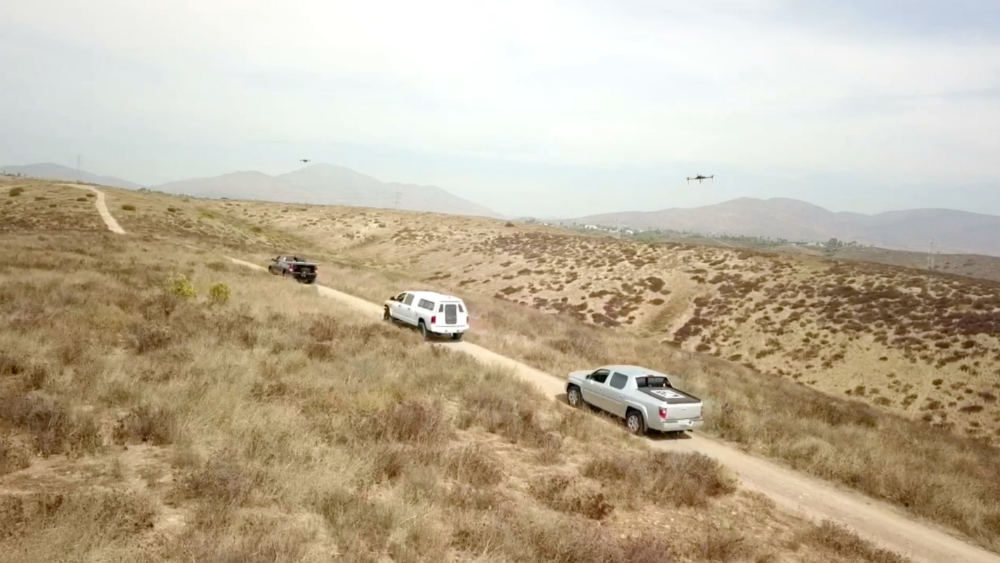
\includegraphics[width=4.5in]{figures/drone_convoy_support.png}
  \caption[UAV Convoy Support]{An example of multirotor UAVs used to increase
  situational awareness for a convoy of
vehicles~\cite{ground_vehicle_based_drones}.}
%
  \label{fig:drone_convoy_support}
\end{figure}

State-of-the-art autonomous vehicle systems require robust solutions to three
problems: state estimation, motion planning and control. In this thesis,
we propose solutions to two of those three problems, state estimation and
control, for a multirotor UAV landing on a moving vehicle.
% We leave the problem
% of motion planning as future work, providing some suggested direction
% in~\secref{sec:future_work}.

\section{Background}

While autonomous landing of multirotor UAVs onto moving vehicles has been
demonstrated in a variety of scenarios~\cite{wynn2019visual}, many problems still remain to
create a truly robust solution. Here we detail several of these outstanding
problems as they relate to the specifc fields of state estimation, motion
planning, and control.

\subsection{State Estimation}
Most low-cost landing methods assume that the landing vehicle is equipped with a
fiducial marker, such as that shown in~\figref{fig:aruco_tag}, that serves as
the designated landing pad for the UAV.
In these methods, a camera mounted to the UAV detects the fiducial landing marker, providing
information about the relative position of the UAV to the landing
vehicle~\cite{borowczyk2017autonomous}. These measurements are often used in a
filtering framework, such as a Kalman filter~\cite{kalman}, to produce a
continous estimate of the relative state between the UAV and the landing
vehicle. However, during landing, it is likely
that the fiducial marker is not detected for periods of time due to occlusion,
sun glare, or UAV motion. For this reason, it is important that the relative
motion between the landing vehicle and the UAV is modeled and used to predict
the relative state when the fiducial marker is not detected.
Even with a good model though,
these methods quickly fail when the fiducial landing
marker is not detected for several seconds~\cite{ling2014precision}.

\begin{figure}[h]
  \centering
  
\includegraphics[width=2.5in]{figures/aruco_104.png}
  \caption[Visual Fiducial Landing Marker]{Visual fiducial markers such as this
    ArUco tag~\cite{garrido2016generation} are commonly used to assist in the
  landing of multirotor UAVs onto moving vehicles.}
  \label{fig:aruco_tag}
\end{figure}

When landing in challenging conditions such as strong winds, bright sun, or
dense fog, it is very common that the fiducial marker may be undetected by the UAV
for long periods of time. Therefore, to create a truly robust landing solution,
the state estimation solution must maintain an accurate estimate of the relative
state between the UAV and the landing vehicle when the fiducial landing marker
is not detected for significant durations. Chapter~\ref{chp:estimation_paper}
describes an estimation algorithm, based on the error-state Kalman
filter~\cite{roumeliotis1999circumventing}, that tracks and estimates the locations of
visual features on the landing vehicle to achieve this goal.

Visual feature
tracking and estimation is a common technique in the field of visual
odometry~\cite{qin2018vins}, however, almost all implementations assume that the
tracked visual features are static with respect to an inertial reference frame.
In the landing scenario, the landing vehicle occupies progressively more of the
field of view of the UAV's camera as the UAV descends. We also note that in most
applications, more precise state estimates are required the closer the UAV gets
to the landing vehicle. For these reasons, the described estimation algorithm
only tracks and estimates visual features that are rigidly attached to the landing vehicle.
Experimental results
from both simulation and hardware demonstrate accurate and consistent estimates
result from the proposed algorithm even when the fiducial marker is undetected
for long periods of time.

\subsection{Motion Planning}
The motion planning problem associated with autonomous vehicles is especially
important when the path the vehicle takes is critical.
This is commonly the case when
navigating close to obstacles. In the case of landing on moving vehicles, it is
often desired that the UAV descends vertically on the landing pad to avoid
potential obstacles including buildings, terrain, or vehicle superstructure.
When landing on certain vehicles, such as a boat at sea, the specific time of
touchdown may also be important to minimize the risk of damage to the UAV.

Much work has been previously presented in the field of motion planning for
small, multirotor UAVs~\cite{mellinger2011minimum}. Specific methods have also been 
presented to generate paths for a UAV landing on a moving
vehicle using model-predictive control in real time~\cite{baca2019autonomous}.
It is likely that one or more of these solutions may be sufficient to create a
robust landing system.
While we do not propose any improvements to these methods in this thesis, we
describe some potential directions for future work related to motion planning
in~\secref{sec:future_work}.

\subsection{Control}
A wide variety of control schemes for multirotor UAVs have been presented over
the past two decades.
A controller to robustly landing a UAV onto a moving vehicle should be able to
closely track a time-dependent trajectory as described in the previous section.
While many previously presented control algorithms may satisfy the
requirements for robust landing on moving vehicles, there has recently been a
movement in the robotics community to appropriately deal with the evolution of a
robot's state along a manifold using Lie theory~\cite{sola2018micro}. Though
these methods have been widely used in the field of state
estimation~\cite{sola2017quaternion, koch2017relative}, there has not been much
work done applying Lie theory to optimal control.

Chapter~\ref{chp:control_paper} of this thesis derives a
linear-quadratic regulator (LQR) using Lie theory that computes control based on
the error-state dynamics of the system. Not only is this a more principled
approach, but it also achieves significant gains in computational efficiency.
Simulation and hardware results show that the derived controller can accurately
track a time-dependent trajectory, making it a good candidate for use in a
robust landing system.

\section{Summary of Contributions}
The research described in this thesis makes two significant contributions:
\begin{itemize}
\item A method of state estimation is developed that maintains accurate and
  consistent estimates of the state of a landing vehicle even when a fiducial landing
  marker is not detected for significant periods of time by a multirotor UAV.
\item An optimal control scheme for a multirotor UAV is derived in an error-state, linear
  quadratic regulator (LQR) formulation. This provides an optimal control scheme
  for a multirotor to follow any dynamically feasible, time-dependent
  trajectory.
\end{itemize}

These contributions were demonstrated in both simulation and hardware
experiments found in Chapters~\ref{chp:estimation_paper}
and~\ref{chp:control_paper}. These results give us reason to believe that a
complete and robust landing solution could be created by combining the proposed
state estimation and control schemes with a competent motion planner.

\section{Thesis Outline}

The remainder of this thesis is organized as follows.
Chapter~\ref{chp:experimental_apparatus} details the hardware and software
systems used
in the experiments. Chapter~\ref{chp:estimation_paper} describes the state
estimation algorithm that maintains accurate and consistent estimates even when
a fiducial landing marker is not detected for significant periods of time.
Chapter~\ref{chp:control_paper} derives an error-state LQR controller for a
multirotor UAV following a dynamically feasible, time-dependent trajectory.
Chapter~\ref{chp:conclusion} provides some concluding remarks including
suggestions for future work that can build upon the work described in this
thesis.

% !TEX root=../master.tex

\chapter{Experimental Apparatus}
\label{chp:experimental_apparatus}

This chapter describes the software and hardware used in the experiments that
are detailed in Chapters~\ref{chp:estimation_paper} and~\ref{chp:control_paper}.

\section{Software}
\subsection {Robot Operating System}
The same C++ algorithm implementations were used both in hardware and simulation
experiments.
This was made possible, in part, due to the use of the Robot Operating System\footnote{Robot Operating System:
\href{www.ros.org}{www.ros.org}} (ROS) as a middleware. ROS provides a way for separate
programs, or nodes, to share information between one another.

A network diagram of the software system can be seen in~\figref{fig:network_diagram}. The estimator and
controller for the UAV were implemented as two separate nodes. 
The estimator node provided the state estimate of the UAV to the controller node.
The controller node computed the desired control action based on the error
between the estimated state and the desired state. This desired control action
was sent to the ROSflight flight control stack~\cite{jackson2016rosflight}
which then actuated either a simulated UAV or the UAV hardware platform.

\begin{figure}[htbp]
  \centering
  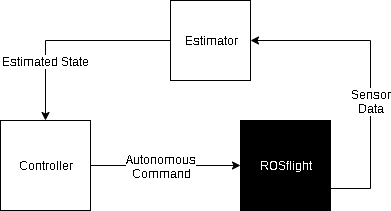
\includegraphics[width=3.5in]{figures/roscopter.png}
  \caption[Software Architecture Network Diagram]{A network diagram of the
  software running during both simulation and hardware experiments.}
%
  \label{fig:network_diagram}
\end{figure}

\subsection {Gazebo}
For simulation experiments, the Gazebo\footnote{Gazebo:
\href{www.gazebosim.org}{www.gazebosim.org}} simulation environment was used with the ROSflight software-in-the-loop
(SIL) simulation.
% This SIL simulation meant that not only the same estimator and controller nodes
% were running in simulation as in hardware, but also the same software from the
% flight controller.
This simulation setup provided for an easier transition from software
experiments to
hardware experiments.

% This simulation setup allowed the
% same estimator and controller implementations to
% be used in the simulation experiments as are used in the hardware experiments,
% making the transition from simulation to hardware less difficult.

\subsection {ROScopter}
The estimator and controller nodes of the ROScopter\footnote{ROScopter:
\href{www.github.com/byu-magicc/roscopter}{www.github.com/byu-magicc/roscopter}}
project were also used during certain points of the simulation and hardware
experiments described in this thesis. In the experiments of the estimator proposed in
Chapter~\ref{chp:estimation_paper}, the ROScopter controller node was used to
close the loop around the produced estimates. In the experiments of the 
controller proposed in Chapter~\ref{chp:control_paper}, the ROScopter estimator node
was used to provide state estimates of the UAV to the controller.

\section{Hardware}
The multirotor UAV used in hardware experiments can be seen
in~\figref{f:drone_pic}. The UAV was built on a DJI Flamewheel 450 frame.
Specific components contained on the UAV are detailed in the following
subsections.

\subsection{Flight Controller}
The multirotor UAV was equipped with an OpenPilot CC3D Revolution 32 bit F4
flight controller as shown in~\figref{fig:f4}. The flight controller ran the
ROSflight firmware which provided an easy interface
for the controller node on the onboard computer to control the UAV.

\begin{figure}[htbp]
  \centering
  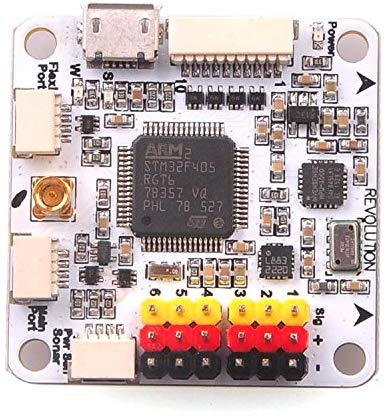
\includegraphics[width=2.5in]{figures/f4.jpg}
  \caption[OpenPilot CC3D Revolution 32 bit F4]{OpenPilot CC3D Revolution 32
    bit F4 flight controller. \\ \hspace{\textwidth} Source:~\cite{openpilotrevo}
}
%
  \label{fig:f4}
\end{figure}

\subsection{Onboard Computer}
The computer onboard the UAV was an NVIDIA Jetson TX2 equipped with an Orbitty
carrier board. This configuration is shown in~\figref{fig:tx2_orbitty}. All
computation was done on the onboard computer during the hardware experiments.

\begin{figure}[h]
  \centering
  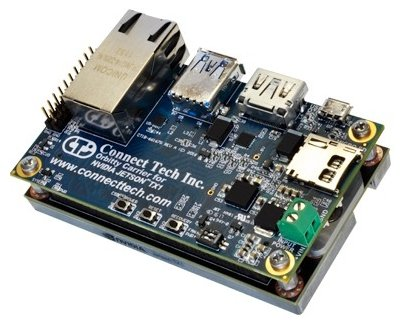
\includegraphics[width=2.5in]{figures/tx2_orbitty.jpg}
  \caption[NVIDIA Jetson TX2 with Orbitty Carrier Board]{NVIDIA Jetson TX2
  with an Orbitty carrier board attached. \\\hspace{\textwidth} Source:~\cite{orbitty}
  }
  \label{fig:tx2_orbitty}
\end{figure}

\subsection{Motion Capture}
Hardware flight experiments were performed in the motion capture room in the
MAGICC Lab at Brigham Young University. This room is equipped with an OptiTrack\footnote{OptiTrack:
\href{www.optitrack.com}{www.optitrack.com}} motion tracking system that
provided high-rate measurements of the position and attitude of the multirotor
UAV during the experiments.

\subsection{Camera}
For the hardware experiments described in Chapter~\ref{chp:estimation_paper},
the multirotor UAV was outfitted with an ELP USB camera with a 2.1 mm lens as
shown in~\figref{fig:camera}. The intrinsic parameters of the sensor were
accurately calibrated using a software package provided by ROS\footnote{ROS
camera\_calibration:
\href{wiki.ros.org/camera_calibration}{wiki.ros.org/camera\_calibration}}.
However, the mounting position and attitude of the camera were only roughly
approximated.

\begin{figure}[h]
  \centering
  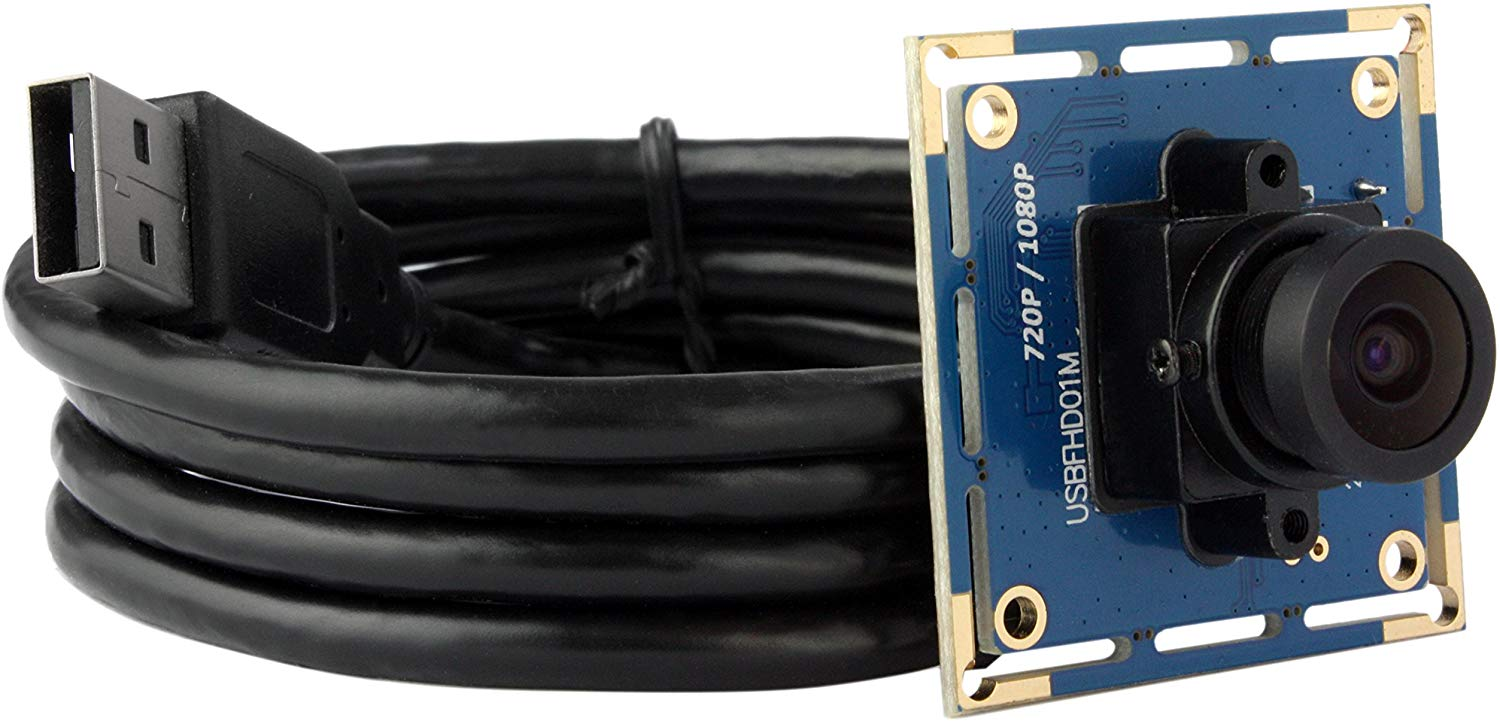
\includegraphics[width=2.5in]{figures/camera.jpg}
  \caption[ELP USB Camera with 2.1 mm Lens]{ELP USB Camera with a 2.1 mm
  lens.

  Source:~\cite{webcam}
}
%
  \label{fig:camera}
\end{figure}


% !TEX root=../master.tex

\chapter[Improving State Estimation of a Landing Target Vehicle
From a Multirotor UAV Using Feature Tracking]{Improving State Estimation of a
  Landing Target Vehicle From a Multirotor UAV Using Feature
Tracking\protect\footnotemark}
\footnotetext{This chapter is a
modified version of the paper to be submitted to the 2020 International Conference on
Unmanned Aircraft Systems, written by Michael Farrell
and Tim McLain.
}
\label{chp:estimation_paper}

\graphicspath{{estimation_paper/}}

\section{Introduction} \label{sec:intro}
% !TEX root=../../master.tex

Small multirotor unmanned air vehicles (UAVs) have rapidly become popular platforms for
a variety of applications including
inspection, reconnaissance, and search and rescue.
% The ability of small multirotor UAVs to agily operate in confined spaces and to
% take off and land vertically give them a unique advantage over other robotic
% platforms.
For many of these use cases, UAVs are required to operate
autonomously, as skilled pilots are not feasible
since they are often unable to maintain direct line of sight to the UAV.
% due to
% limitations in line of sight. 
% A variety of emerging use cases
% require multirotor UAVs to operate from larger, mobile vehicles.
% a moving vehicle.
% instead of from the static world.
% These use
% cases include martitime surveillance, where the UAV must operate from
% a martitime vessel at sea,
% and package delivery, where the UAV must operate from a large truck in motion.
Newly emerging use cases such as maritime surveillance and package delivery
pose unique problems, requiring UAVs to operate autonomously from larger,
mobile vehicles instead of from a stationary base station.
% require UAVs to operate autonomously from larger, mobile vehicles.
% which carries the packages to be delivered.
% The ability to operate reliably from a
% moving vehicle is still a very active field of research, posing many unsolved
% problems.

% \cite{ling2014precision} AprilTag, kalman filter to predict
% \cite{araar2017vision} relies on a known map of many AprilTags fiducials.
% \cite{borowczyk2017autonomous} uses a single AprilTag, fast car
% \cite{baca2019autonomous} main MBZIRC 2017 paper (tag = square with x)
% \cite{falanga2017vision} MBZIRC, SVO + IMU
% \cite{beul2017fast} MBZIRC
% \cite{cantelli2017autonomous} MBZIRC
% \cite{marantos2018vision} helicopter, tag (Aruco/April)

% \cite{lee2012autonomous} IBVS
% \cite{wynn2019visual} IBVS - nested tag

Nearly all current approaches to the operation of multirotor UAVs with respect to moving
vehicles rely on the
% A variety of approaches to the operation of multirotor UAVs with respect to
% moving vehicles have been proposed in literature.
% Nearly all of these approaches rely on the
detection of a fiducial marker on the moving vehicle for relative pose
measurements. One of the earliest of these works
used a known configuration of infrared LEDs on the landing vehicle as a fiducial
marker~\cite{wenzel2011automatic}.
% relied on the detection of infrared LEDs that were
% illuminated in a known configuration on the landing
% vehicle~\cite{wenzel2011automatic}.
Since then, visual fiducial markers such as
AprilTags~\cite{olson2011tags} and ArUco markers~\cite{garrido2016generation}
have become more widely
used~\cite{ling2014precision,borowczyk2017autonomous,marantos2018vision,
araar2017vision}.
% In 2017, the Mohamed Bin Zayed International Robotics Challenge (MBZIRC)
% featured a stage that included landing a multirotor UAV on a visual fiducial
% marker atop a moving golf
% cart~\cite{baca2019autonomous,falanga2017vision,beul2017fast,cantelli2017autonomous}.
% While some landing methods employ image-based visual
% servoing~\cite{lee2012autonomous,wynn2019visual}, most methods
% require an estimate of the state of the target landing vehicle.
While some landing methods control the UAV entirely based on the detections of the
fiducial marker~\cite{lee2012autonomous,wynn2019visual}, more robust methods
compute control based on an estimate of the state of the target landing
vehicle~\cite{ling2014precision}.

% The Kalman filter~\cite{kalman} is a widely used algorithm 
% As we should not expect uninterrupted detection of the fiducial marker during
% landing, it is
% important to model the dynamics of the target vehicle and use them to propagate
% forward
As the UAV descends toward the landing target, it is common
that the fiducial marker remains undetected
% to not detect the fiducial marker
for periods of time due to poor lighting, occlusion, or extreme
motion.
% For this reason, it is important that a model of the dynamics of the target vehicle
For this reason, it is important that the dynamics of the target vehicle are
modeled and
used by the estimation algorithm to predict the state of the target vehicle
when measurements are not available.
The Kalman filter~\cite{kalman} has been frequently used
for this task, producing accurate estimates 
% showing good results 
when the fiducial marker is not detected for
short periods of time~\cite{baca2019autonomous}.
% n estimation method which models
% the dynamics of the target vehicle is employed to maintain accurate estimates in
% between measurements.
% Ling notes in~\cite{ling2014precision} that it is important to model the
% dynamics of the target vehicle so that they can be propagated forward for short
% periods of time when the fiducial marker is not
% detected.
Due to imperfect motion models, however,
all of the mentioned
approaches are likely to fail if the fiducial marker is not detected for
significant periods of time.
% due to imperfect motion models.
% because the target vehicle is likely to not
% perfectly follow the modeled motion.
% Even if the state of the target vehicle is estimated, the estimates are only as
% good as the
% motion model of the target vehicle when the fiducial marker is not detected.
% We propose an improvement to these methods: 
% To improve these methods, we propose an estimation algorithm that detects,
% tracks, and estimates the positions of unknown visual features on the target
% vehicle in addition to the fiducial marker.
To improve these methods, we propose an estimation algorithm that uses
measurements of unknown visual features on the target vehicle in addition to
measurements resulting from detections of a fiducial marker.
% to improve
% estimation accuracy when the fiducial marker is not detected for significant
% periods of time.

% Tracking and estimating the positions of visual features is
% a common technique used
% % similar to that commonly used
% in the field of visual odometry.
Many visual odometry methods such
as~\cite{qin2018vins,leutenegger2013keyframe,mourikis2007multi,mur2015orb} use
detected and tracked visual features to aid in camera motion estimation.
% as VINS-MONO, OKVIS, MSCKF, and ORB SLAM use an indirect approach
% \cite{qin2018vins} VINS-MONO, feature extraction, optical flow frame to frame
% \cite{leutenegger2013keyframe} OKVIS, BRISK features
% \cite{mourikis2007multi} MSCKF, uses SIFT features
% \cite{mur2015orb} ORB SLAM
In these methods, the tracked visual features are assumed to belong to the
static world.
Visual odometry techniques
% tracking static features
have also been previously applied to landing on
moving platforms~\cite{falanga2017vision}.
During landing, however, static features become more sparse as the dynamic target vehicle
occupies progessively more of the
field of view of the UAV's camera. This results in detoriating
estimates as the UAV approaches the landing target.
% During landing, however, it is common for the target vehicle to occupy the
% entire field of view of the UAV's camera, making it impossible to track static
% features throughout the duration of the flight.
% While visual odometry techniques have been
% previously applied to landing on
% moving platforms~\cite{falanga2017vision}, these methods still only tracked and
% estimated static features.
% During the landing phase, it is not uncommon, however, for the target vehicle
% to occupy the entire field of view of the UAV's camera, making it not possible
% to track static features throughout the duration of the flight.
For this reason, the proposed estimator, instead, tracks and estimates the
locations of
visual features that are rigidly attached to the target vehicle. These tracked
visual features provide information about the relative position of the target
vehicle
as long as the vehicle remains in the field of view of the camera.
% for the duration of the flight.
% movement of the UAV as well as
% information about the movement of the target vehicle.
We show in simulation and hardware experiments that the estimation of these tracked features allows
for accurate estimates of the state of the target vehicle even
when the fiducial marker is not detected for significant periods of time.


% !TEX root=../root.tex

The outline of this chapter is as follows.
\secref{sec:math_prelim} explains the mathematical notation and conventions used
throughout the chapter.
\secref{sec:estimation} presents the proposed estimation algorithm including the
state dynamics, state initialization and measurement models.
\secref{sec:est_paper_simulation} describes the simulation experiments conducted and
\secref{sec:est_paper_hardware} describes the hardware experiments conducted.
\secref{sec:est_paper_conclusion} provides concluding remarks.


\section{Mathematical Preliminaries} \label{sec:model}
% !TEX root=../root.tex

\subsection{Notation}

Throughout the paper, we represent vectors with a bold letter (e.g., $\bf v$)
and matrices with a captial letter (e.g., $A$). Other common notation used
throughout the paper is contained below.
\begin{center}
\begin{tabularx}{\columnwidth}{lX}
$R_a^b$ & Rotation matrix from reference frame $a$ to $b$ \\
$\vect{v}_{a/b}^c$ & Vector state $\vect{v}$ of frame $a$ w.r.t.~frame $b$, expressed in frame $c$ \\
$\hat{a}$ & Estimate of true variable $a$ \\
$\bar{a}$ & Measurement of $a$ \\
% $\des{a}$ & Desired value of $a$ \\
$\dot{a}$ & Time derivative of $a$ \\
$\tilde{a}$ & Error of variable $a$, i.e., $\tilde{a} \triangleq a - \hat{a}$
\end{tabularx}
\end{center}
%
We also make use of the following coordinate frames:
\begin{center}
\begin{tabularx}{\columnwidth}{lX}
$I$ & The inertial coordinate frame in north-east-down\\
% $\ell$ & The aircraft's vehicle-1 (body-level) coordinate frame \\
$v$ & The aircraft's vehicle-1 (body-level) coordinate frame \\
$b$ & The aircraft's body-fixed coordinate frame \\
$c$ & The camera frame \\
$g$ & The target landing vehicle's body-fixed coordinate frame located at the desired
landing location (goal) of the aircraft
\end{tabularx}
\end{center}
%
We use the standard basis vectors $\vect{e}_1, \vect{e}_2, \vect{e}_3$,
where $\vect{e}_1 = \begin{bmatrix} 1 & 0 & 0 \end{bmatrix}^\transpose$,
$\vect{e}_2 = \begin{bmatrix} 0 & 1 & 0 \end{bmatrix}^\transpose$,
and $\vect{e}_3 = \begin{bmatrix} 0 & 0 & 1 \end{bmatrix}^\transpose$.
We also use the skew-symmetric matrix operator
% We make frequent use of the skew-symmetric matrix operator defined by
\begin{equation}
  \skewmat{\vect{v}} \triangleq
  \begin{bmatrix}
  0 & -v_{3} & v_{2}\\
  v_{3} & 0 & -v_{1}\\
  -v_{2} & v_{1} & 0
  \end{bmatrix},
\end{equation}
which is related to the cross-product between two vectors as
\begin{equation}
  \vect{v}\times\vect{w}=\skewmat{\vect{v}}\vect{w},
\end{equation}
and the skew-symmetric identity
\begin{equation}
  \skewmat{\vect{v}} \vect{w} = -\skewmat{\vect{w}} \vect{v}.
\end{equation}
We also use the two-dimensional skew-symmetric operator which acts on a scalar
\begin{equation}
  \skewmat{a} \triangleq
  \begin{bmatrix}
  0 & -a \\
  a & 0
  \end{bmatrix}.
\end{equation}
We use the identity matrix, $I$, as well as submatricies of $I$ denoted with
subscripts such as
\begin{equation}
  I_{2 \times 3} =
  \begin{bmatrix}
    1 & 0 & 0 \\
    0 & 1 & 0
  \end{bmatrix}.
\end{equation}

% !TEX root=../root.tex

\subsection{Quaternion Representation}
% \MF{TODO what of this is necessary}
% A quaternion $\q$ is a hyper-complex number of rank four.  It is well known that
% a unit quaternion $\in S^3$ can be used to efficiently represent attitude, as
% $S^3$ is a double cover of $\SO(3)$.  Quaternions have the advantage over
% $\SO(3)$ of being more efficient to implement on modern hardware~\cite{casey2013AttitudeRepresentation}, therefore in the software implementation of the described algorithm, we use quaternions, rather than rotation matrices.

% We use the Hamiltonian notation for unit quaternions $\in S^3$
Unit quaternions $\in S^3$ throughout the paper follow the Hamiltonian notation
\begin{equation}
  % \q=\begin{pmatrix}q_{0} & q_{x}i & q_{y} j & q_{z} k \end{pmatrix}.%=\begin{pmatrix}q_{0} & \bar{\q} \end{pmatrix},
  \q= q_{0} + q_{x}i + q_{y} j + q_{z} k .%=\begin{pmatrix}q_{0} & \bar{\q} \end{pmatrix},
\end{equation}
where $i$, $j$, and $k$ are the fundamental quaternion units.
% We write the complex p
% For convenience, we sometimes refer to the complex portion of the quaternion as
% \begin{equation}
	% \bar{\q} = \begin{bmatrix} q_x & q_y & q_z \end{bmatrix} ^\transpose
% \end{equation}
% and write quaternions as the tuple of the real and complex portions
We write quaternions as the tuple
\begin{equation}
	\q = \begin{pmatrix} q_0 \\ \bar{\q} \end{pmatrix}
\end{equation}
where $q_0$ represents the real portion of the quaternion and
% and the complex
% portion of the quaternion is given by
\begin{equation}
	\bar{\q} = \begin{bmatrix} q_x & q_y & q_z \end{bmatrix} ^\transpose
\end{equation}
respresents the complex portion of the quaternion.

% Given our use of the Hamiltonian notation, the quaternion group operator
Given this representation of the quaternion, the quaternion group operator
$\otimes$ can be written as the matrix-like products
\begin{align}
  \q^a \otimes \q^b &= \begin{pmatrix} q_0^a & \left(-\bar{\q}^{a}\right)^\transpose \\ \bar{\q}^a & q^a_0 I + \skewmat{\bar{\q}^a} \end{pmatrix}
	\begin{pmatrix} q_0^b \\ \bar{\q}^b\end{pmatrix}
  \label{eq:quat_otimes_product1} \\
  &= \begin{pmatrix} q_0^b & \left(-\bar{\q}^{b}\right)^\transpose \\ \bar{\q}^b & q^b_0 I - \skewmat{\bar{\q}^b} \end{pmatrix}
	\begin{pmatrix} q_0^a \\ \bar{\q}^a \end{pmatrix}.
  \label{eq:quat_otimes_product2}
\end{align}
% It is often convenient to convert a quaternion $\q$ to its associated passive rotation matrix.  This is done with
We frequently convert a quaternion $\q$ to its associated passive rotation
matrix. This is done with
\begin{equation}
R\left(\q\right)=\left(2q_{0}^{2}-1\right)I-2q_{0}\skewmat{\bar{\q}}+2\bar{\q}\bar{\q}^{\top}\in SO\left(3\right).
\label{eq:est_paper_R_from_q}
\end{equation}
We also note that rotations are written equivalently as
$\q_a^b=R\left(\q_a^b\right)=R_a^b$ throughout the paper.
% where the choice of these is dictated by convenience.
% We use passive rotation matrices, meaning that the rotation matrix $R_a^b$ acts
% on a vector $\vect{r}^a$, expressed in frame $a$, and results in the same
% vector, now expressed in frame $b$ as
% \begin{equation}
% \vect{r}^b = R_a^b \vect{r}^a .
% \end{equation}

% We need to frequently convert between the Lie group, $S^3$, and the Lie
% algebra, $\mathbb{R}^3$, which enables us to operate in a vector space.
To operate in a vector space, we frequently convert between the Lie group,
$S^3$,
% and the Lie algebra, $\mathbb{R}^3$.
and the vector space, $\mathbb{R}^3$, that is isomorphic to the Lie algebra.
This is done with the
exponential and logarithmic mappings. The exponential mapping for a unit quaternion is defined as
\begin{align}
\exp_{\q} & :\mathbb{R}^{3}\rightarrow S^3\nonumber \\
\exp_{\q}\left(\vect{\delta}\right) & \triangleq\begin{bmatrix}\cos\left(\frac{\lVert\vect{\delta}\rVert}{2}\right)\\
\sin\left(\frac{\lVert\vect{\delta}\rVert}{2}\right)\frac{\vect{\delta}}{\lVert\vect{\delta}\rVert}
\end{bmatrix},\label{eqn:exponential_map}
\end{align}
with the corresponding logarithmic map defined as
\begin{align}
\log_{\q} & :S^3\rightarrow \mathbb{R}^{3}\nonumber \\
\log_{\q}\left(\q\right) & \triangleq2\;\mathrm{atan2}\left(\left\Vert \bar{\q}\right\Vert ,q_{0}\right)\frac{\bar{\q}}{\left\Vert \bar{\q}\right\Vert }.\label{eqn:log_map}
\end{align}
% To avoid numerical issues when $\norm{\vect{\delta}}\approx0$, we also employ the small-angle approximations of the quaternion exponential and logarithm
With this formulation, $\vect{\delta}$ also represents the axis-angle
representation of a rotation where the unit vector
$\frac{\vect{\delta}}{\norm{\vect{\delta}}}$ represents the axis of rotation,
and $\norm{\vect{\delta}}$ represents the angular magnitude of rotation.
When $\norm{\vect{\delta}}\approx0$,
we employ the small-angle approximations of the quaternion exponential and
logarithm given by
\begin{align}
\exp_{\q}\left(\vect{\delta}\right) & \approx\begin{bmatrix}1\\
\frac{\vect{\delta}}{2}
\end{bmatrix}\label{eq:est_paper_quaternion_exp_approx}\\
\log_{\q}\left(\q\right) & \approx2\;\textrm{sign}\left(q_{0}\right)\bar{\q}.\label{eq:quaternion_log_approx}
\end{align}


% The $\boxplus$/$\boxminus$ notation for unit quaternions is now defined by
% \begin{align*}
% \boxplus: & S^3\times\mathbb{R}^{3}\rightarrow S^3\\
%  & \q\boxplus\vect{\delta}\triangleq\q\otimes\exp_q\left(\vect{\delta}\right)\\
% \boxminus: & S^3\times S^3\rightarrow\mathbb{R}^{3}\\
%  & \q\boxminus\vect{p}\triangleq\log_q\left(\vect{p}^{-1}\otimes\q\right).
% \end{align*}
% Let's look at one application for clarification.
% With body angular rate $\vect{\omega}_{b/i}^b$, inertial to body rotation $\q_i^b$, and $\vect{\theta}=\vect{\omega}_{b/i}^b \Delta t$, we have
% \begin{align}
% \q_i^b\left(t+\Delta t\right) & =\q_i^b\left(t\right)\boxplus\vect{\theta}\\
% \vect{\theta} & =\q_i^b\left(t+\Delta t\right)\boxminus\q_i^b\left(t\right).
% \end{align}

%\subsection{Quadrotor Dynamics With Quaternion Attitude}
%In the associated software library, we employ the following dynamics for the quadrotor:
%\begin{align}
    %\dot{\vect{p}}_{b/I}^{I} &= 	R\left(\q_{I}^{b}\right)^\transpose \vect{v}_{b/I}^{b} \nonumber \\
	%\dot{\q}_{I}^{b} &= - \frac{1}{2} \begin{pmatrix} 0 \\ \omega_{b/I}^b\end{pmatrix} \otimes \q_I^b\nonumber\\
	%\dot{\vect{v}}_{b/I}^{b} 
	%&= 	g\frac{s}{s_e}\vect{e}_3 + gR\left(\q_I^b\right) \vect{e}_3- \drag\vect{v}_{b/I}^b - \skewmat{\vect{\omega}_{b/I}^b}\vect{v}_{b/I}^b.
	%\label{eq:quat_dynamics}
%\end{align}
%and we solve this using a fourth-order Runge-Kutta extension of \eqref{eq:quaternion_integration}.

% TODO maybe pull from here
%\subsection{Quaternion Error State Dynamics}
%As with the rotation matrix, we wish to find a minimal representation of the error about a quaternion attitude state.  Let us start with the differential equation for quaternion dynamics
%\begin{equation}
	%\dot{\q}_{I}^{b} = \frac{1}{2}\q_I^b \otimes \begin{pmatrix} 0 \\ \vect{\omega}_{b/I}^b\end{pmatrix}.
%\end{equation}
%This can be solved using the quaternion exponential with
%\begin{equation}
	%\q_I^b\left(t\right) = \q_I^b\left(0\right)\otimes\exp_{\q}\left(\int_0^t \vect{\omega}_{b/I}^b\left(\tau\right) d\tau \right).
%\end{equation}
%To reduce this to our minimal vector representation, as we did with rotation matrices in \eqref{eq:att_vector}, let us define the attitude vector $\vect{r}_I^b\left(t\right)=\vect{r}_I^b\left(t_0\right)+\int_{t_0}^t\boldsymbol{\omega}_{b/I}^b\left(\tau\right)d\tau$ with $\vect{r}_I^b\left(t_0\right)=0$ such that
%\begin{equation}
	%\q_I^b\left(t\right) = \q_I^b\left(0\right)\otimes\exp_{\q}\left(\vect{r}_I^b\left(t\right) \right).
%\end{equation}
%It then follows that the error state of our attitude vector is
%\begin{align}
	%\tilde{\vect{r}}_I^{b} 
		%&= \vect{r}_I^b - \hat{\vect{r}}_I^{\hat{b}}  \nonumber \\
		%&= \vect{r}_I^b - R\left(\q_I^b\right) R\left(\q_I^{\hat{b}}\right)^\transpose \hat{\vect{r}}_I^{\hat{b}}\nonumber \\
		%&= \vect{r}_I^b - R\left(\tilde{\q}_{\hat{b}}^b\right)  \hat{\vect{r}}_I^{\hat{b}}
%\end{align}
%and its time derivative is
%\begin{equation}
	%\dot{\tilde{\vect{r}}}_I^{b} = \dot{\vect{r}}_I^b - R\left(\tilde{\q}_{\hat{b}}^b\right)  \dot{\hat{\vect{r}}}_I^{\hat{b}}.
%\end{equation}
%\subsection{Quaternion Trajectory Generation}
%When creating trajectories using differential flatness for quaternion attitude states, the equivalent expression to \eqref{eq:des_attitude} is
%\begin{equation}
	%\des{q}_I^b = \exp_{\q}\left(\vect{e}_3\des{\psi}_{b/I}^I)\right) \otimes \exp_{\q}\left(\theta \vect{\delta}\right) \label{eq:des_attitude}
%\end{equation}
%where, as in \eqref{eq:des_attitude}, $\theta\vect{\delta}$ is the axis-angle error between the desired acceleration and the inertial z-axis.

% TEX root=../root.tex

\subsection{Planar Rotations}
\label{sec:planar_rotations}
% \subsection{2D Rotation Group}
% We use rotation matrices, the Lie group $SO(2)$, to represent 2D rotations.
% We parameterize the 2D rotation matrix by the angle, $\psi$, such that
% \begin{align}
  % \begin{array}{llll}
    % R &= \exp_R \left( \psi \right) &=
  % \begin{bmatrix}
    % \cos \psi & - \sin \psi \\
    % \sin \psi & \cos \psi
  % \end{bmatrix} & \in \mathbb{R}^{2 \times 2} \\
    % \psi &= \log_R \left( \psi \right) &= \mathrm{atan2} \left(r_{21},r_{11}
      % \right) & \in \mathbb{R}.
  % \end{array}
% \end{align}
% We also note that planar rotations are commutative, meaning
% \begin{equation}
  % R_b^c R_a^b = R_a^b R_b^c \qquad \forall R_a^b, R_b^c \in SO(2).
% \end{equation}

% We parameterize the 2D rotation group as an angle, $\psi$, which respresents
We parameterize planar rotations as an angle, $\psi$, which respresents
the angle of rotation about a given axis.
% We treat $\psi$ as a vector space
% that uses the common addition and subtraction operators such that
We treat $\psi \in \mathbb{R}^1$ so that common addition and subtraction
operators can be used such as
\begin{align}
  \psi_a^c &= \psi_a^b + \psi_b^c \\
  \psi_a^b &= \psi_a^c - \psi_b^c.
\end{align}
We note, however, that with this formulation, all addition and subtraction
operations must be wrapped such
that the resultant angle $\psi \in \left[ \right. -\pi, \pi \left. \right)$. The
passive 2D
rotation matrix can be created from any $\psi$ as
\begin{equation}
  R \left( \psi \right) = \begin{bmatrix} \cos \psi & -\sin \psi \\ \sin \psi &
  \cos \psi \end{bmatrix}.
\end{equation}
If $\psi$ represents the angle of rotation about the $z$ axis of a reference frame, then
the corresponding passive 3D rotation matrix is given by
\begin{equation}
  R \left( \psi \right) = \begin{bmatrix}
    \cos \psi & -\sin \psi & 0 \\
    \sin \psi & \cos \psi & 0 \\
    0 & 0 & 1
  \end{bmatrix}.
\end{equation}

% We treat S1 as a vector space but make sure to wrap residuals between -pi and
% pi. 
% Also a 2D rotation matrix can be made like this...
% And a 3D rotation matrix like this..


\section{Estimation} \label{sec:estimation}
% !TEX root=./root.tex

% The propsed estimator estimates both the state of
% the UAV and the state of the target vehicle as well as the positions of visual
% landmarks on the target vehicle.
% in the same Error-State Kalman
% filter~\cite{sola2017quaternion}.
% Though
% This work focuses on the estimation of the state of a landing target
% vehicle. However, we also estimate the state of the UAV to properly account for the
% uncertainty in the UAV states that appear in the motion model of the target
% vehicle and the measurement
% models used. states upon which many of the measurement models depend.
This work focuses on the estimation of the state of the landing target vehicle.
However, as several of the measurement models employed depend on the state of the
UAV, we also estimate the state of the UAV in the same filter to properly
account for the uncertainty in its state.
We, therefore, estimate the position, attitude, and velocity of the UAV given by
$\hat{\vect{p}}_{b/I}^{I}$, $\hat{\vect{q}}_I^{b}$, and
$\hat{\vect{v}}_{b/I}^b$.
In addition, we estimate bias states for the acclerometer and gyroscope sensors that are
used as inputs to the filter. These estimated states are given by
$\hat{\vect{\beta}}_a$ and $\hat{\vect{\beta}}_{\omega}$.

The estimated state of the target vehicle is defined as the position, velocity,
attitude, and angular rate of the target vehicle.
% denoted by
% $\hat{\vect{p}}_{g/b}^{v}$, $\hat{\vect{v}}_{g/I}^{g}$, $\hat{\psi}_{I}^{g}$,
% and $\hat{\omega}_{g/I}^{g}$.
We note that the
estimated position of the target vehicle, $\hat{\vect{p}}_{g/b}^v$, is relative to the position of the
UAV.
We formulate this state relatively,
as this relative state is observable even with poor estimates of the UAV's global
position, $\hat{\vect{p}}_{b/I}^I$, due to the relative information provided
by the measurements as described in~\secref{sec:measurement_models}.
For this work, we assume that the target vehicle's
motion is constrained to a two-dimensional plane. This means that the estimated
target vehicle velocity, $\hat{\vect{v}}_{g/I}^{g}$, is only of two dimensions and that the
estimated attitude, $\hat{\psi}_{I}^g$, represents a planar rotation as
described in~\secref{sec:planar_rotations}, implying that the estimated angular
rate, $\hat{\omega}_{g/I}^g$ is of one dimension.

As previously mentioned, we also estimate the locations of unknown visual
features on the target vehicle.
The vectors $\hat{\vect{r}}_{1/g}^{g}, \dots \hat{\vect{r}}_{n/g}^{g}$ represent the
estimated locations of visual features $1, \dots n$ with respect to the goal frame and
expressed in the goal frame. As we assume these features are rigidly attached to the
target vehicle, these vectors remain constant as the vehicle moves and rotates.
We show in the experiments described in~\secref{sec:est_paper_simulation}
and~\secref{sec:est_paper_hardware} that the
addition of only ten visual features to the estimated state significantly
improves the estimates of the state of the target vehicle
% $\hat{\x}_{\text{Goal}}$
while the fiducial landing marker is not detected. 

% We, therefore, estimate the position,
% attitude, and velocity of the UAV together with the position, attitude, velocity,
% and angular rate of the target vehicle and the positions of visual features on
% the target vehicle. We also estimate bias states for the
% accelerometer and gyroscope sensors that are used as inputs to the filter.
% to properly
% account for the uncertainty, as several of the 
We express the full state of the estimated system as the tuple
\begin{equation}
  \hat{\x} =
  \begin{pmatrix}
    \hat{\x}_{\text{UAV}}, \hat{\x}_{\text{Goal}}, \hat{\x}_{\text{Features}}
  \end{pmatrix}
\end{equation}
with the components defined as
\begin{align}
  \hat{\vect{x}}_{\text{UAV}} &=
  \begin{pmatrix}
    \hat{\vect{p}}_{b/I}^{I}, \hat{\vect{q}}_I^{b}, \hat{\vect{v}}_{b/I}^b,
    \hat{\vect{\beta}}_a,
    \hat{\vect{\beta}}_{\omega}
  \end{pmatrix}
    \in \mathbb{R}^3 \times S^3 \times \mathbb{R}^3 \times \mathbb{R}^3 \times
    \mathbb{R}^3  \\
  % \x_{\text{UAV}} &=
  % \begin{bmatrix}
    % \vect{p}_{b/I}^I &
    % \phi & \theta & \psi &
    % \vect{v}_{b/I}^b &
    % \mu & \vect{\beta}_a & \vect{\beta}_\omega
  % \end{bmatrix}^\transpose \\
    \hat{\x}_{\text{Goal}} & =
    \begin{pmatrix}
      \hat{\vect{p}}_{g/b}^{v}, \hat{\vect{v}}_{g/I}^{g}, \hat{\psi}_{I}^{g},
      \hat{\omega}_{g/I}^{g}
    \end{pmatrix}
    \in \mathbb{R}^3 \times \mathbb{R}^2 \times \mathbb{R}^1 \times \mathbb{R}^1
    \\
    \hat{\x}_{\text{Features}} & =
    \begin{pmatrix}
      \hat{\vect{r}}_{1/g}^{g}, \dots \hat{\vect{r}}_{n/g}^{g}
    \end{pmatrix}
    \in \mathbb{R}^3 \times \dots \mathbb{R}^3.
\end{align}
The inputs to the estimated system are given by
\begin{equation}
  \vect{u} = \begin{pmatrix} \bar{\vect{a}}_{b/I}^b, \bar{\vect{\omega}}_{b/I}^b \end{pmatrix} \in
        \mathbb{R}^3 \times \mathbb{R}^3,
\end{equation}
which are directly measured from an inertial measurement unit mounted on the UAV.
% Though
% this work focuses on the estimation of the state of the landing target
% vehicle, we also estimate the state of the UAV to properly account for the
% uncertainty in these states upon which the motion model for
% $\x_{\text{Goal}}$ and many of the measurement models depend.

% The estimated states associated with the UAV, $\hat{\vect{x}}_{\text{UAV}}$,
% contain the traditionally estimated states of position, attitude, and velocity
% in addition to bias states for the accelerometer and gyroscope sensors.

% The estimated states associated with the target vehicle,
% $\hat{\vect{x}}_{\text{Goal}}$, contain the position, attitude, velocity, and
% angular velocity of the target vehicle.
% We note that the
% estimated position of the target vehicle, $\hat{\vect{p}}_{g/b}^v$, is relative to the position of the
% UAV.
% We formulate this state relatively,
% as this relative state is observable even with poor estimates of the UAV's global
% position, $\hat{\vect{p}}_{g/I}^I$, due to the relative information provided
% by the measurements as described in~\secref{sec:measurement_models}.
% Note that $\hat{\vect{x}}_{\text{UAV}}$ contains the same states mentioned previously
% in~\secref{sec:UAV_dynamics} with the addition of $\hat{\vect{\beta}}_a$ and
% $\hat{\vect{\beta}}_\omega$, the estimated bias vectors for the acclerometer and
% gyroscope sensors. On the
% other hand, $\hat{\vect{x}}_{\text{Goal}}$ varies 
% from the target vehicle states mentioned in~\secref{sec:landing_veh_dynamics}
% by containing $\hat{\vect{p}}_{g/b}^v$ instead of $\hat{\vect{p}}_{b/I}^I$.
% % as well as $\hat{\vect{r}}_{1/g}^{g} \dots \hat{\vect{r}}_{n/g}^{g}$.
% We estimate the relative state, $\hat{\vect{p}}_{g/b}^v$, instead
% of the global state, $\hat{\vect{p}}_{g/I}^I$, as the relative state is observable
% even with poor estimates of the UAV's global position, $\hat{\vect{p}}_{b/I}^I$.

% The estimated vectors $\hat{\vect{r}}_{1/g}^{g}, \dots \hat{\vect{r}}_{n/g}^{g}$ represent the
% locations of visual features $1, \dots n$ with respect to the goal frame and
% expressed in the goal frame. As we assume these features are rigidly attached to the
% target vehicle, these vectors remain constant as the vehicle moves and rotates.
% We show in the experiments described in~\secref{sec:est_paper_simulation}
% and~\secref{sec:est_paper_hardware} that the
% addition of only ten visual features to the estimated state significantly
% improves the estimates of the state of the target vehicle
% % $\hat{\x}_{\text{Goal}}$
% while the fiducial landing marker is not detected. 

We also note
that the estimated state is of dynamic size. As visual features are
detected they are added to the estimated state until a maximum size of the state
is reached. As visual features leave the field of view of the camera,
or are otherwise no longer tracked, they are removed from the estimated state
to make room for new visual features to be added.

% In the following
% subsections, we define the error-state of the estimated system,  thdescribe the dynamic equations used to model the state of the
% estimated system, the
% initialization of certain states, and the specific
% measurement models used to update the filter.

% As mentioned in~\secref{sec:intro??} the estimation of these
% visual landmarks allows the estimator to maintain accurate and consistent
% estimates of the target vehicle even while the fiducial landing marker is not
% detected for long periods of time.

\subsection{Error-State Definition}

As the estimated state is not a vector, but rather a tuple of Lie groups, we
employ the error-state Kalman filter (ESKF) as described in~\cite{koch2017relative}.
% The error-state of the estimated system is defined by
We define the error-state of the estimated system as
\begin{align}
  \tilde{\vect{x}} =&
  \left[ \begin{matrix}
    \tilde{\vect{p}}_{b/I}^{I}, \tilde{\vect{\theta}}_I^{b}, \tilde{\vect{v}}_{b/I}^b,
    \tilde{\vect{\beta}}_a,
    \tilde{\vect{\beta}}_{\omega},
    \tilde{\vect{p}}_{g/b}^{v}, \tilde{\vect{v}}_{g/I}^{g}, \tilde{\psi}_{I}^{g},
    \tilde{\omega}_{g/I}^{g},
      \tilde{\vect{r}}_{1/g}^{g}, \dots \tilde{\vect{r}}_{n/g}^{g}
  \end{matrix} \right]
  \in \mathbb{R}^{22 + 3n}
\end{align}
with the error-state components related to the vector states, $\x_{\vect{v}}$, defined with
the vector subtraction operator as
\begin{equation}
\tilde{\x}_{\vect{v}} \triangleq \x_{\vect{v}} - \hat{\x}_{\vect{v}}
\label{eq:est_paper_vector_error_state}
\end{equation}
such that
\begin{equation}
  \tilde{\vect{p}}_{b/I}^I = \vect{p}_{b/I}^I - \hat{\vect{p}}_{b/I}^I.
  \label{eq:est_paper_uav_pos_err_state}
\end{equation}
We reiterate that we treat $\psi_I^g \in \mathbb{R}^1$
% as a vector space
such that
\begin{equation}
  \tilde{\psi}_I^g = \psi_I^g - \hat{\psi}_I^g.
  \label{eq:2d_att_err_state}
\end{equation}

We follow~\cite{koch2017relative}, defining the error-state of the quaternion,
$\q_I^b$,
as the minimal representation
\begin{equation}
  \tilde{\vect{\theta}}_I^b \triangleq \log_{\q} \left( \left( \hat{\q}_I^b \right)^{-1}
  \otimes \q_I^b \right)
  \label{eq:quat_error_state}
\end{equation}
which implies
\begin{equation}
  \q_I^b  = \hat{\q}_I^b \otimes \exp_{\q} \left( \tilde{\vect{\theta}}_I^b
  \right).
  \label{eq:quat_true_state}
\end{equation}
As rotation matrices concatenate in the order opposite to
quaternions,~\eqref{eq:quat_true_state} can also be expressed as
\begin{equation}
  R_I^b  = R \left( \exp_{\q} \left( \tilde{\vect{\theta}}_I^b \right) \right)
  \hat{R}_I^b.
  \label{eq:rot_true_state}
\end{equation}
% Similarly, we define the error-state of the 2D rotation matrix state, $R_I^g$,
% as
% \begin{equation}
  % \tilde{\psi}_I^g = \log_R \left(  
  % R_I^g \left( \hat{R}_I^g \right)^\transpose \right)
  % \label{eq:2d_rot_err_state}
% \end{equation}

To derive the error-state dynamics and the measurement residual Jacobians in the
following sections, we
use an approximation for~\eqref{eq:rot_true_state} developed by first expanding
the
quaternion exponential using~\eqref{eq:est_paper_quaternion_exp_approx} as
$\tilde{\vect{\theta}}_I^b$ is assumed to be small
\begin{equation}
  R_I^b  \approx R \left( \begin{bmatrix}
      1 \\
    \frac{1}{2} \tilde{\vect{\theta}}_I^b
  \end{bmatrix}\right)
  \hat{R}_I^b.
\end{equation}
We then employ~\eqref{eq:est_paper_R_from_q}, neglecting higher-order terms, to
yield the approximation
\begin{equation}
  R_I^b  \approx 
  \left( I - \skewmat{\tilde{\vect{\theta}}_I^b} \right)
  \hat{R}_I^b.
  \label{eq:est_paper_Rapprox}
\end{equation}
It can similarly be shown that
\begin{equation}
  \left( R_I^b \right)^\transpose  \approx 
  \left( \hat{R}_I^b \right)^\transpose
  \left( I + \skewmat{\tilde{\vect{\theta}}_I^b} \right).
  \label{eq:est_paper_RTapprox}
\end{equation}




% !TEX root=./root.tex

\subsection{Propagation Model}
To model the motion of the UAV, we use common rigid-body kinematics given by
% We use common rigid body kinematics to model the dynamics of
% the UAV given by
\begin{align}
  \dot{\vect{p}}_{b/I}^I
  &=
  \left( R_I^b \right)^\transpose \vect{v}_{b/I}^b
  \label{eq:uav_dynamics}
  \\
  \dot{\vect{q}}_{I}^{b} 
	&= 	
  \q_I^b \otimes \begin{pmatrix} 0 \\ \frac{1}{2}
    \left( \bar{\vect{\omega}}_{b/I}^b - \vect{\beta}_\omega - \vect{\upsilon}_\omega \right)
\end{pmatrix} \nonumber \\
  \dot{\vect{v}}_{b/I}^b 
  &=
  R_I^b \vect{g}^I
  +
  \skewmat{\vect{v}_{b/I}^b}
  \left( \bar{\vect{\omega}}_{b/I}^b - \vect{\beta}_\omega -
  \vect{\upsilon}_\omega \right)
  +
  \left( \bar{\vect{a}}_{b/I}^b - \vect{\beta}_a - \vect{\upsilon}_a \right) \nonumber
  % \vect{\eta}_v 
  \\
  \dot{\vect{\beta}}_a &= \vect{\eta}_{\beta_a} \nonumber
  \\
  \dot{\vect{\beta}}_\omega &= \vect{\eta}_{\beta_\omega}, \nonumber
\end{align}
% $\vect{\eta}_v$, 
where $\vect{g}^I$ represents the gravity vector expressed in the inertial
frame, $\vect{\eta}_{\beta_a}$ and $\vect{\eta}_{\beta_\omega}$ are zero-mean
Gaussian noise processes corresponding to the state dynamics, and
$\vect{\upsilon}_\omega$ and $\vect{\upsilon}_a$ are zero-mean Gaussian noise
processes corresponding to the noise in the inputs to the system.

We model the motion of the landing target vehicle
with a constant-velocity and constant-angular-velocity motion model such that
% Though this is a very simplified model, we show
% in~\secref{sec:simulation} and~\secref{sec:hardware} that it is sufficient for
% cases that do not perfectly match this model. The dynamics of $\x_{\text{Goal}}$ are expressed as
% \begin{align}
  % \dot{\hat{\vect{p}}}_{g/b}^{v} &= \left( \hat{R}_{I}^{g} \right)^\transpose
  % \hat{\vect{v}}_{g/I}^{g} - \left( \hat{R}_{I}^{b} \right)^\transpose
  % \hat{\vect{v}}_{b/I}^{b} \label{eq:goal_dynamics} \\
  % \dot{\hat{\vect{v}}}_{g/I}^{g} &= \vect{0} \nonumber \\
  % \dot{\hat{\theta}}_{I}^{g} &= \hat{\omega}_{g/I}^g \nonumber \\
  % \dot{\hat{\omega}}_{g/I}^{g} &= 0. \nonumber
% \end{align}
\begin{align}
  \dot{\vect{p}}_{g/b}^{v} &= I_{3 \times 2} \left( R_{I}^{g} \right)^\transpose
   \vect{v}_{g/I}^{g} - \left( R_{I}^{b} \right)^\transpose
  \vect{v}_{b/I}^{b} \label{eq:goal_dynamics} \\
  \dot{\vect{v}}_{g/I}^{g} &= \vect{\eta}_{gv} \nonumber \\
  \dot{\psi}_{I}^{g} &= \omega_{g/I}^g \nonumber \\
  % \dot{R}_{I}^{g} &= -\skewmat{ \omega_{g/I}^g } R_I^g \nonumber \\
  \dot{\omega}_{g/I}^{g} &= \eta_{g\omega}, \nonumber
\end{align}
where $\vect{\eta}_{gv}$ and $\eta_{g\omega}$ are zero-mean Gaussian noise
processes. Though this is a simplified motion model for the target
vehicle, we show in~\secref{sec:est_paper_simulation}
and~\secref{sec:est_paper_hardware} that it is
satisfactory for our experiments. We intend the motion model of the target
vehicle to be easily modified for vehicles with more complex motion such
as a boat at sea.

As mentioned previously, we assume the tracked visual features are rigidly
attached to the landing vehicle such that
% there are no dynamics 
% of their associated states
\begin{equation}
  \dot{\vect{r}}_{i/g}^g = \vect{0}. \label{eq:feature_dynamics}
  % \dot{\hat{\vect{r}}}_{i/g}^g = \vect{0}. \label{eq:feature_dynamics}
\end{equation}

In the ESKF, the estimated state is propagated independently of the filter using
the expected value of the modeled dynamics. We use the expected values
of~\eqref{eq:uav_dynamics}, \eqref{eq:goal_dynamics}, and
\eqref{eq:feature_dynamics} given by
% The estimated state is propagated
\begin{align}
  \dot{\hat{\vect{p}}}_{b/I}^I
  &=
  \left( \hat{R}_I^b \right)^\transpose \hat{\vect{v}}_{b/I}^b
  \label{eq:estimated_dynamics}
  \\
  \dot{\hat{\vect{q}}}_{I}^{b} 
  &= 	
  \hat{\q}_I^b \otimes \begin{pmatrix} 0 \\ \frac{1}{2}
  \left( \bar{\vect{\omega}}_{b/I}^b - \hat{\vect{\beta}}_\omega \right)
\end{pmatrix} \nonumber \\
  \dot{\hat{\vect{v}}}_{b/I}^b 
  &=
  \hat{R}_I^b \vect{g}^I
  +
  \skewmat{\hat{\vect{v}}_{b/I}^b}
  \left( \bar{\vect{\omega}}_{b/I}^b - \hat{\vect{\beta}}_\omega \right)
  +
  \left( \bar{\vect{a}}_{b/I}^b - \hat{\vect{\beta}}_a \right) \nonumber
  \\
  \dot{\hat{\vect{\beta}}}_a &= \vect{0} \nonumber
  \\
  \dot{\hat{\vect{\beta}}}_\omega &= \vect{0} \nonumber
  \\
  \dot{\hat{\vect{p}}}_{g/b}^{v} &= I_{3 \times 2} \left( \hat{R}_{I}^{g} \right)^\transpose
   \hat{\vect{v}}_{g/I}^{g} - \left( \hat{R}_{I}^{b} \right)^\transpose
  \hat{\vect{v}}_{b/I}^{b} \nonumber \\
  \dot{\hat{\vect{v}}}_{g/I}^{g} &= \vect{0} \nonumber \\
  \dot{\hat{\psi}}_{I}^{g} &= \hat{\omega}_{g/I}^g \nonumber \\
  % \dot{\hat{R}}_{I}^{g} &= -\skewmat{ \hat{\omega}_{g/I}^g } \hat{R}_I^g \nonumber \\
  \dot{\hat{\omega}}_{g/I}^{g} &= 0 \nonumber \\
  \dot{\hat{\vect{r}}}_{i/g}^g &= \vect{0}. \nonumber
\end{align}

The error-state dynamics used to propagate the filter are found by relating
the modeled true-state dynamics from~\eqref{eq:uav_dynamics},
\eqref{eq:goal_dynamics}, and \eqref{eq:feature_dynamics}
with~\eqref{eq:estimated_dynamics} using the error-state definitions
from~\eqref{eq:est_paper_vector_error_state} and~\eqref{eq:quat_error_state}. The
first-order approximation of the error-state dynamics is given by 
\begin{align}
  \dot{\tilde{\vect{p}}}_{b/I}^I
  &\approx
  \left( \hat{R}_I^b \right)^\transpose \tilde{\vect{v}}_{b/I}^b
  - \left( \hat{R}_I^b \right)^\transpose \skewmat{\hat{\vect{v}}_{b/I}^b}
  \tilde{\vect{\theta}}_I^b
  \\
  \dot{\tilde{\vect{\theta}}}_{I}^{b} 
  &\approx 	
  -\skewmat{ \bar{\vect{\omega}}_{b/I}^b - \hat{\vect{\beta}}_\omega}
    \tilde{\vect{\theta}}_I^b
    - \tilde{\vect{\beta}}_\omega -
    \vect{\upsilon}_\omega
  \nonumber \\
  \dot{\tilde{\vect{v}}}_{b/I}^b 
  &\approx
  \skewmat{ \hat{R}_I^b \vect{g}^I } \tilde{\vect{\theta}}_I^b 
  -
  \skewmat{ \hat{\vect{v}}_{b/I}^b } \tilde{\vect{\beta}}_\omega
  -
  \skewmat{ \hat{\vect{v}}_{b/I}^b } \vect{\upsilon}_\omega
  -
  \skewmat{ \bar{\omega}_{b/I}^b - \hat{\vect{\beta}}_\omega }
  \tilde{\vect{v}}_{b/I}^b
  -
  \tilde{\vect{\beta}}_a
  -
  \vect{\upsilon}_a \nonumber
  \\
  \dot{\tilde{\vect{\beta}}}_a &= \vect{\eta}_{\beta_a} \nonumber
  \\
  \dot{\tilde{\vect{\beta}}}_\omega &= \vect{\eta}_{\beta_\omega} \nonumber
  \\
  \dot{\tilde{\vect{p}}}_{g/b}^{v}
                                  &\approx
  I_{3 \times 2} \left( \hat{R}_{I}^{g} \right)^\transpose
  \tilde{\vect{v}}_{g/I}^g
  +
  I_{3 \times 2} \left( \hat{R}_{I}^{g} \right)^\transpose
  \skewmat{ \tilde{\psi}_I^g } \hat{\vect{v}}_{g/I}^g
  +
  \left( \hat{R}_{I}^{b} \right)^\transpose \skewmat{ \hat{\vect{v}}_{b/I}^{b} } 
  \tilde{\vect{\theta}}_I^b
  -
  \left( \hat{R}_{I}^{b} \right)^\transpose \tilde{\vect{v}}_{b/I}^{b} \nonumber \\
  \dot{\tilde{\vect{v}}}_{g/I}^{g} &= \vect{\eta}_{gv} \nonumber \\
  \dot{\tilde{\psi}}_{I}^{g} &= \tilde{\omega}_{g/I}^g \nonumber \\
  \dot{\tilde{\omega}}_{g/I}^{g} &= \eta_{g\omega} \nonumber \\
  \dot{\tilde{\vect{r}}}_{i/g}^g &= \vect{0}, \nonumber
\end{align}
or succinctly,
\begin{equation}
  \dot{\tilde{\x}} = f\left(\x, \tilde{\x}, \vect{u}, \tilde{\vect{u}}\right).
\end{equation}
The derivation of these error-state dynamics can be found in
Appendix~\ref{apdx:estimation_err_state_derivation}. In practice, the expected
value of the error state remains zero over the propagation window, and only the
error covariance, $P$, is propagated.
The continous-time derivative of the error covariance is given by
% forward using a first-order approximation
% of the continous-time derivative of covariance given by
\begin{equation}
  \dot{P} = FP + PF^\transpose + G Q_{\vect{u}} G^\transpose + Q_{\vect{x}}
  % P^{+} = FP + PF^\transpose + G Q_{\vect{u}} G^\transpose + Q_{\vect{x}}
\end{equation}
where $Q_{\vect{u}}$ is the input noise covariance, $Q_{\vect{x}}$ is the
process noise covariance,
% \MF{TODO define this matrix by vertical slices}
% \begin{align}
  % F &= \frac{ \partial \dot{\tilde{\x}} }{ \partial \tilde{\x} } \\
    % &=
    % \scriptsize
    % \begin{bmatrix}
    % % \begin{smallbmatrix}
      % \vect{0} & - \left( \hat{R}_I^b \right)^\transpose
      % \skewmat{\hat{\vect{v}}_{b/I}^b} & \left( \hat{R}_I^b \right)^\transpose &
      % \vect{0} & \vect{0} & \vect{0} & \vect{0}
               % & 0 & 0 & \vect{0} \\
      % \vect{0} & -\skewmat{ \bar{\vect{\omega}}_{b/I}^b
      % - \hat{\vect{\beta}}_\omega} & \vect{0} & \vect{0} & -I & \vect{0} & \vect{0}
               % & 0 & 0 & \vect{0} \\
      % \vect{0} & \skewmat{ \hat{R}_I^b \vect{g} } &
      % -\skewmat{ \bar{\omega}_{b/I}^b - \hat{\vect{\beta}}_\omega } & -I &
      % -\skewmat{ \hat{\vect{v}}_{b/I}^b } & \vect{0} & \vect{0}
               % & 0 & 0 & \vect{0} \\
      % \vect{0} & \vect{0} & \vect{0} & \vect{0} & \vect{0} & \vect{0} & \vect{0}
               % & 0 & 0 & \vect{0} \\
      % \vect{0} & \vect{0} & \vect{0} & \vect{0} & \vect{0} & \vect{0} & \vect{0}
               % & 0 & 0 & \vect{0} \\
      % \vect{0} & \left( \hat{R}_{I}^{b} \right)^\transpose
      % \skewmat{ \hat{\vect{v}}_{b/I}^{b} } & 
      % -\left( \hat{R}_{I}^{b} \right)^\transpose & \vect{0} & \vect{0} & \vect{0} & 
      % I_{3 \times 2} \left( \hat{R}_{I}^{g} \right)^\transpose
               % & I_{3 \times 2} \left( \hat{R}_{I}^{g} \right)^\transpose
               % \skewmat{ 1 } \hat{\vect{v}}_{g/I}^g
               % & 0 & \vect{0} \\
      % \vect{0} & \vect{0} & \vect{0} & \vect{0} & \vect{0} & \vect{0} & \vect{0}
               % & 0 & 0 & \vect{0} \\
      % \vect{0} & \vect{0} & \vect{0} & \vect{0} & \vect{0} & \vect{0} & \vect{0}
               % & 0 & 1 & \vect{0} \\
      % \vect{0} & \vect{0} & \vect{0} & \vect{0} & \vect{0} & \vect{0} & \vect{0}
               % & 0 & 0 & \vect{0} \\
      % \vect{0} & \vect{0} & \vect{0} & \vect{0} & \vect{0} & \vect{0} & \vect{0}
               % & 0 & 0 & \vect{0}
    % \end{bmatrix},
    % % \end{smallbmatrix},
% \end{align}
\begin{align}
  F &= \frac{ \partial \dot{\tilde{\x}} }{ \partial \tilde{\x} } \\
    &=
    \begin{bmatrix}
      \vect{0} &
    \cfrac{ \partial \dot{\tilde{\vect{p}}}_{b/I}^{I}}{ \partial \tilde{\vect{\theta}}_I^{b}}
      % - \left( \hat{R}_I^b \right)^\transpose
      % \skewmat{\hat{\vect{v}}_{b/I}^b}
               &
      % \left( \hat{R}_I^b \right)^\transpose
               \cfrac{ \partial \dot{\tilde{\vect{p}}}_{b/I}^{I} }{ \partial \tilde{\vect{v}}_{b/I}^b }
               &
      \vect{0} & \vect{0} & \vect{0} & \vect{0}
               & \vect{0} & \vect{0} & \vect{0} & \dots & \vect{0} \\
      \vect{0} &
      % -\skewmat{ \bar{\vect{\omega}}_{b/I}^b
      % - \hat{\vect{\beta}}_\omega}
      \cfrac{ \partial \dot{\tilde{\vect{\theta}}}_I^{b} }{ \partial \tilde{\vect{\theta}}_I^{b} }
               & \vect{0} & \vect{0} &
      \cfrac{ \partial \dot{\tilde{\vect{\theta}}}_I^{b} }{ \partial \tilde{\vect{\beta}}_{\omega} }
      % -I
               & \vect{0} & \vect{0}
               & \vect{0} & \vect{0} & \vect{0} & \dots & \vect{0} \\
      \vect{0} &
      % \skewmat{ \hat{R}_I^b \vect{g} }
      \cfrac{ \partial \dot{\tilde{\vect{v}}}_{b/I}^b }{ \partial \tilde{\vect{\theta}}_I^{b} }
               &
      % -\skewmat{ \bar{\omega}_{b/I}^b - \hat{\vect{\beta}}_\omega }
      \cfrac{ \partial \dot{\tilde{\vect{v}}}_{b/I}^b }{ \partial \tilde{\vect{v}}_{b/I}^b }
               &
      \cfrac{ \partial \dot{\tilde{\vect{v}}}_{b/I}^b }{ \partial \tilde{\vect{\beta}}_a }
      % -I
               &
      \cfrac{ \partial \dot{\tilde{\vect{v}}}_{b/I}^b }{ \partial \tilde{\vect{\beta}}_{\omega} }
      % -\skewmat{ \hat{\vect{v}}_{b/I}^b }
               & \vect{0} & \vect{0}
               & \vect{0} & \vect{0} & \vect{0} & \dots & \vect{0} \\
      \vect{0} & \vect{0} & \vect{0} & \vect{0} & \vect{0} & \vect{0} & \vect{0}
               & \vect{0} & \vect{0} & \vect{0} & \dots & \vect{0} \\
      \vect{0} & \vect{0} & \vect{0} & \vect{0} & \vect{0} & \vect{0} & \vect{0}
               & \vect{0} & \vect{0} & \vect{0} & \dots & \vect{0} \\
      \vect{0} &
      % \left( \hat{R}_{I}^{b} \right)^\transpose
      % \skewmat{ \hat{\vect{v}}_{b/I}^{b} }
      \cfrac{ \partial \dot{\tilde{\vect{p}}}_{g/b}^{v} }{ \partial \tilde{\vect{\theta}}_I^{b} }
               & 
      % -\left( \hat{R}_{I}^{b} \right)^\transpose
      \cfrac{ \partial \dot{\tilde{\vect{p}}}_{g/b}^{v} }{ \partial \tilde{\vect{v}}_{b/I}^b }
               & \vect{0} & \vect{0} & \vect{0} & 
      % I_{3 \times 2} \left( \hat{R}_{I}^{g} \right)^\transpose
      \cfrac{ \partial \dot{\tilde{\vect{p}}}_{g/b}^{v} }{ \partial \tilde{\vect{v}}_{g/I}^{g} }
               &
               % I_{3 \times 2} \left( \hat{R}_{I}^{g} \right)^\transpose
               % \skewmat{ 1 } \hat{\vect{v}}_{g/I}^g
      \cfrac{ \partial \dot{\tilde{\vect{p}}}_{g/b}^{v} }{ \partial \tilde{\psi}_{I}^{g} }
               & \vect{0} & \vect{0} & \dots & \vect{0} \\
      \vect{0} & \vect{0} & \vect{0} & \vect{0} & \vect{0} & \vect{0} & \vect{0}
               & \vect{0} & \vect{0} & \vect{0} & \dots & \vect{0} \\
      \vect{0} & \vect{0} & \vect{0} & \vect{0} & \vect{0} & \vect{0} & \vect{0}
               & 0 & 
      % 1 
               \cfrac{ \partial \dot{\tilde{\psi}}_{I}^{g} }{ \partial \tilde{\omega}_{g/I}^{g} }
               & \vect{0} & \dots & \vect{0} \\
      \vect{0} & \vect{0} & \vect{0} & \vect{0} & \vect{0} & \vect{0} & \vect{0}
               & 0 & 0 & \vect{0} & \dots & \vect{0} \\
      \vect{0} & \vect{0} & \vect{0} & \vect{0} & \vect{0} & \vect{0} & \vect{0}
               & \vect{0} & \vect{0} & \vect{0} & \dots & \vect{0} \\
      \vdots & \vdots & \vdots & \vdots & \vdots & \vdots & \vdots
             & \vdots & \vdots & \vdots & \ddots & \vdots \\
      \vect{0} & \vect{0} & \vect{0} & \vect{0} & \vect{0} & \vect{0} & \vect{0}
               & \vect{0} & \vect{0} & \vect{0} & \dots & \vect{0}
    \end{bmatrix},
\end{align}
with
\begin{align}
    \cfrac{ \partial \dot{\tilde{\vect{p}}}_{b/I}^{I}}{ \partial \tilde{\vect{\theta}}_I^{b}}
    &=
      - \left( \hat{R}_I^b \right)^\transpose
      \skewmat{\hat{\vect{v}}_{b/I}^b} \\
               \cfrac{ \partial \dot{\tilde{\vect{p}}}_{b/I}^{I} }{ \partial \tilde{\vect{v}}_{b/I}^b }
    &=
      \left( \hat{R}_I^b \right)^\transpose \\
      \cfrac{ \partial \dot{\tilde{\vect{\theta}}}_I^{b} }{ \partial \tilde{\vect{\theta}}_I^{b} }
    &=
      -\skewmat{ \bar{\vect{\omega}}_{b/I}^b
      - \hat{\vect{\beta}}_\omega}
\end{align}
\begin{align}
      \cfrac{ \partial \dot{\tilde{\vect{\theta}}}_I^{b} }{ \partial \tilde{\vect{\beta}}_{\omega} }
    &=
      -I \\
      \cfrac{ \partial \dot{\tilde{\vect{v}}}_{b/I}^b }{ \partial \tilde{\vect{\theta}}_I^{b} }
    &=
      \skewmat{ \hat{R}_I^b \vect{g} } \\
      \cfrac{ \partial \dot{\tilde{\vect{v}}}_{b/I}^b }{ \partial \tilde{\vect{v}}_{b/I}^b }
    &=
      -\skewmat{ \bar{\omega}_{b/I}^b - \hat{\vect{\beta}}_\omega } \\
      \cfrac{ \partial \dot{\tilde{\vect{v}}}_{b/I}^b }{ \partial \tilde{\vect{\beta}}_a }
    &=
      -I \\
      \cfrac{ \partial \dot{\tilde{\vect{v}}}_{b/I}^b }{ \partial \tilde{\vect{\beta}}_{\omega} }
    &=
      -\skewmat{ \hat{\vect{v}}_{b/I}^b } \\
      \cfrac{ \partial \dot{\tilde{\vect{p}}}_{g/b}^{v} }{ \partial \tilde{\vect{\theta}}_I^{b} }
    &=
      \left( \hat{R}_{I}^{b} \right)^\transpose
      \skewmat{ \hat{\vect{v}}_{b/I}^{b} } \\
      \cfrac{ \partial \dot{\tilde{\vect{p}}}_{g/b}^{v} }{ \partial \tilde{\vect{v}}_{b/I}^b }
    &=
      -\left( \hat{R}_{I}^{b} \right)^\transpose \\
      \cfrac{ \partial \dot{\tilde{\vect{p}}}_{g/b}^{v} }{ \partial \tilde{\vect{v}}_{g/I}^{g} }
    &=
      I_{3 \times 2} \left( \hat{R}_{I}^{g} \right)^\transpose \\
      \cfrac{ \partial \dot{\tilde{\vect{p}}}_{g/b}^{v} }{ \partial \tilde{\psi}_{I}^{g} }
    &=
               I_{3 \times 2} \left( \hat{R}_{I}^{g} \right)^\transpose
               \skewmat{ 1 } \hat{\vect{v}}_{g/I}^g \\
               \cfrac{ \partial \dot{\tilde{\psi}}_{I}^{g} }{ \partial \tilde{\omega}_{g/I}^{g} }
    &=
      1 ,
\end{align}
and
\begin{align}
  G &= \frac{ \partial \dot{\tilde{\x}} }{ \partial \vect{\upsilon} } \\
    &=
    \begin{bmatrix}
      \vect{0} & \vect{0} \\
      \vect{0} & -I \\
      -I & -\skewmat{\hat{\vect{v}}_{b/I}^b} \\
      \vect{0} & \vect{0} \\
      \vect{0} & \vect{0} \\
      \vect{0} & \vect{0} \\
      \vect{0} & \vect{0} \\
      \vect{0} & \vect{0} \\
      \vect{0} & \vect{0} \\
      \vect{0} & \vect{0} \\
      \vdots & \vdots \\
      \vect{0} & \vect{0} 
    \end{bmatrix}.
\end{align}
However, to ensure numerical stability, we propagate the covariance using a first-order discrete approximation
defined by
\begin{equation}
  P_{k+1} = F_{k} P_{k} F_{k}^\transpose + G_k Q_u G_k^\transpose + Q_x \Delta
  t^2
\end{equation}
where
\begin{align}
  F_k &\approx I + F \Delta t \\
  G_k &\approx G \Delta t.
\end{align}



% !TEX root=../../master.tex

\subsection{Measurement Models}
\label{sec:measurement_models}

When
updating the filter with measurements, we make use of the partial Kalman update
which has been shown to improve estimates of bias states and constant values~\cite{brink2017partial}. The partial Kalman update provides a
means to limit the effect of measurement updates to certain estimated
states by providing a tuning vector
\begin{equation}
  \vect{\lambda} =
\begin{bmatrix}
  \lambda_1 & \lambda_2 & \dots & \lambda_N
\end{bmatrix}
\end{equation}
where $\lambda_i \in \left[ 0, 1\right]$ determines the proportion of the
measurement update applied to state $i$.
In practice, we use $\lambda < 1$ only for the
bias states, $\vect{\beta}_a$ and $\vect{\beta}_\omega$, and the
constant-value states $\vect{r}_{1/g}^{g}, \dots \vect{r}_{n/g}^{g}$.

With this formulation,
when a measurement is received, we compute the Kalman gain
\begin{equation}
  K = P H^\transpose \left(H P H^\transpose + R \right)^{-1}
\end{equation}
where $H$ is the residual Jacobian for the measurement and $R$ is the
measurement covariance. We then follow~\cite{brink2017partial}, using $K$ to update the filter such that
\begin{align}
  \hat{\tilde{\x}}^{+} &= \vect{\lambda} \odot K \vect{r} \\
  P^{+} &= P + \Lambda \odot \left( \left(I - K H \right) P \left(I - K H
  \right)^\transpose + K R K^\transpose - P \right)
\end{align}
where $\odot$ is the Hadamard product, $\vect{r}$ is the residual of the
measurement and
\begin{align}
  \vect{1} &= \begin{bmatrix} 1 & 1 & \dots & 1 \end{bmatrix}^\transpose \\
  \Lambda &= \vect{1} \vect{\lambda}^\transpose + \vect{\lambda} \vect{1} -
  \vect{\lambda} \vect{\lambda}^\transpose.
\end{align}

As the estimate of the error state of the system, $\hat{\tilde{\x}}$, becomes
non-zero after this update, we use this estimate to correct the estimated state,
$\hat{\x}$. As the estimated state is not a vector, this correction is done
piecewise. The vector components of the estimated state are
updated as
\begin{equation}
  \hat{\vect{\x}}_{\vect{v}}^{+} = \hat{\vect{\x}}_{\vect{v}} + \tilde{\vect{\x}}_{\vect{v}}
\end{equation}
and the quaternion state is updated as
\begin{equation}
  \left( \hat{\q}_I^b \right)^{+}  = \hat{\q}_I^b \otimes \exp_{\q} \left(
  \tilde{\vect{\theta}}_I^b \right).
\end{equation}
After this correction, the estimate of the error state of the system resets to
zero.
% reset to zero.
% The estimate of the error state of the system is then reset to zero before any

The measurement model, residual model and residual
Jacobian are defined below for each type of measurement used in the filter.

\subsubsection{Global UAV Position Measurement}
We assume to receive a measurement of the position of the UAV with respect to
the inertial frame.
In our experiments, this measurement results from a motion capture system;
however, in other applications,
a sensor such as a real-time kinematic GPS unit could provide this measurement.
% a similar measurement can be be used from RTK
% GPS.
% This measurement may come from a sensor such as GPS or a motion capture system.
% The 
% The measurement model and its estimate are
The measurement and its model are
written as
\begin{align}
  \vect{z}_{\text{pos}} &= h_{\text{pos}} \left( \x \right) + \vect{\eta}_{\text{pos}} \\
  h_{\text{pos}} \left( \x \right) &= \vect{p}_{b/I}^I,
  % \vect{\eta}_{\text{pos}},
  % h_{\text{pos}} \left( \hat{\x} \right) &= \hat{\vect{p}}_{b/I}^I,
\end{align}
where $\vect{\eta}_{\text{pos}}$ is a zero-mean Gaussian process
describing the sensor noise.
For a given measurement of position, $\bar{\vect{z}}_{\text{pos}}$, the residual is
given by
\begin{equation}
  \vect{r}_{\text{pos}} = \bar{\vect{z}}_{\text{pos}} - h_{\text{pos}} \left( \hat{\x}
  \right).
\end{equation}
For the error-state Kalman filter, the residual is modeled as
\begin{align}
  % \vect{r}_{\text{pos}} &=  h_{\text{pos}} \left( \x \right) - h_{\text{pos}} \left( \hat{\x}
  % \right) \\
  \vect{r}_{\text{pos}} &=  \vect{z}_{\text{pos}} - h_{\text{pos}} \left( \hat{\x}
  \right) \\
                        &= \vect{p}_{b/I}^I + \eta_{\text{pos}} -
                        \hat{\vect{p}}_{b/I}^I \\
                        &= \tilde{\vect{p}}_{b/I}^I + \eta_{\text{pos}}.
\end{align}
This results in the residual Jacobian
\begin{align}
  H_{\text{pos}} &= \frac{\partial \vect{r}_{\text{pos}}}{\partial \tilde{\x}}\\
                 &=
   \begin{bmatrix}
     \cfrac{\partial \vect{r}_{\text{pos}}}{\partial \tilde{\vect{p}}_{b/I}^{I} } &
     \vect{0} &
     \vect{0} &
     \vect{0} &
     \vect{0} &
     \vect{0} &
     \vect{0} &
     \vect{0} &
     \vect{0} &
     \vect{0} &
     \dots &
     \vect{0}
     % \cfrac{\partial \vect{r}_{\text{pos}}}{\partial \tilde{\vect{\theta}}_I^{b} } &
     % \cfrac{\partial \vect{r}_{\text{pos}}}{\partial \tilde{\vect{v}}_{b/I}^b } &
     % \cfrac{\partial \vect{r}_{\text{pos}}}{\partial \tilde{\vect{\beta}}_a } &
     % \cfrac{\partial \vect{r}_{\text{pos}}}{\partial \tilde{\vect{\beta}}_{\omega} } &
     % \cfrac{\partial \vect{r}_{\text{pos}}}{\partial \tilde{\vect{p}}_{g/b}^{v} } &
     % \cfrac{\partial \vect{r}_{\text{pos}}}{\partial \tilde{\vect{v}}_{g/I}^{g} } &
     % \cfrac{\partial \vect{r}_{\text{pos}}}{\partial \tilde{\psi}_{I}^{g} } &
     % \cfrac{\partial \vect{r}_{\text{pos}}}{\partial \tilde{\omega}_{g/I}^{g} } &
     % \cfrac{\partial \vect{r}_{\text{pos}}}{\partial \tilde{\vect{r}}_{i/g}^{g} }
   \end{bmatrix} \\
                 &=
  \begin{bmatrix}
    I_{3 \times 3} & \vect{0} & \vect{0} & \vect{0} & \vect{0} & \vect{0} &
    \vect{0} & \vect{0} & \vect{0} & \vect{0} & \dots & \vect{0}
  \end{bmatrix}.
\end{align}

% and the non-zero component of the Jacobian of the measurement model as
% \begin{equation}
  % \frac{\partial \hat{\vect{p}}_{b/I}^I}{\partial \vect{p}_{b/I}^I} = I_{3
  % \times 3}.
% \end{equation}

\subsubsection{Global UAV Attitude Measurement}
Similar to the position measurement above, we assume to receive a measurement of
the attitude of the body frame of the UAV with respect to the inertial frame.
In our experiments, this measurement results from a motion capture system;
however, in other applications, a sensor such as an attitude and heading
reference system could provide this measurement.
% This measurement may
% come from an attitude and heading reference system or from a motion
% capture system. 
% The measurement model and its estimate are
The measurement and its model are 
written as
\begin{align}
  \vect{z}_{\text{att}} &= h_{\text{att}} \left( \x \right) \otimes \exp_{\q} \left(
  \vect{\eta}_{\text{att}} \right) \\
  h_{\text{att}} \left( \x \right) &= \vect{q}_{I}^b, 
  % \vect{\eta}_{\text{att}} \right) \\
    % h_{\text{att}} \left( \hat{\x} \right) &= \hat{\vect{q}}_{I}^b,
\end{align}
where $\vect{\eta}_{\text{att}}$ is a zero-mean Gaussian process
describing the sensor noise.
For a given measurement of attitude, $\bar{\vect{z}}_{\text{att}}$, the residual is
given by
\begin{equation}
  \vect{r}_{\text{att}} = \log_{\q} \left(  h_{\text{att}} \left(
  \hat{\x} \right)^{-1} \otimes \bar{\vect{z}}_{\text{att}} \right),
  % \vect{r}_{\text{att}} = \vect{z}_{\text{att}} - h_{\text{att}} \left( \hat{\x}
\end{equation}
which is modeled as
\begin{align}
  \vect{r}_{\text{att}} &= \log_{\q} \left(  h_{\text{att}} \left(
  \hat{\x} \right)^{-1} \otimes \vect{z}_{\text{att}} \right) \\
  % \hat{\x} \right)^{-1} \otimes h_{\text{att}} \left( \x \right) \right) \\
                        &= \log_{\q} \left(  \left(
  \hat{\vect{q}}_{I}^b \right)^{-1} \otimes \vect{q}_{I}^b \otimes \exp_{\q} \left(
  \vect{\eta}_{\text{att}} \right)\right).
\end{align}
This is expanded using~\eqref{eq:quat_true_state} and simplified to yield
\begin{align}
  \vect{r}_{\text{att}}
  % &= \log_{\q} \left(  h_{\text{att}} \left(
  % \hat{\x} \right)^{-1} \otimes h_{\text{att}} \left( \x \right) \right) \\
                        % &= \log_{\q} \left(  \left(
  % \hat{\vect{q}}_{I}^b \right)^{-1} \otimes \vect{q}_{I}^b \otimes \exp_{\q} \left(
  % \vect{\eta}_{\text{att}} \right)\right) \\
                        &= \log_{\q} \left(  \left(
                        \hat{\vect{q}}_{I}^b \right)^{-1} \otimes
                        \hat{\vect{q}}_{I}^b \otimes \exp_{\q} \left(
                      \tilde{\vect{\theta}}_I^b \right) \right)
                          + \vect{\eta}_{\text{att}}  \\
                        &= \tilde{\vect{\theta}}_I^b
                          + \vect{\eta}_{\text{att}}. 
\end{align}
This results in the residual Jacobian
\begin{align}
  H_{\text{att}} &= \frac{\partial \vect{r}_{\text{att}}}{\partial \tilde{\x}}\\
                 &=
   \begin{bmatrix}
     \vect{0} &
     \cfrac{\partial \vect{r}_{\text{att}}}{\partial \tilde{\vect{\theta}}_I^{b} } &
     \vect{0} &
     \vect{0} &
     \vect{0} &
     \vect{0} &
     \vect{0} &
     \vect{0} &
     \vect{0} &
     \vect{0} &
     \dots &
     \vect{0}
     % \cfrac{\partial \vect{r}_{\text{pos}}}{\partial \tilde{\vect{\theta}}_I^{b} } &
     % \cfrac{\partial \vect{r}_{\text{pos}}}{\partial \tilde{\vect{v}}_{b/I}^b } &
     % \cfrac{\partial \vect{r}_{\text{pos}}}{\partial \tilde{\vect{\beta}}_a } &
     % \cfrac{\partial \vect{r}_{\text{pos}}}{\partial \tilde{\vect{\beta}}_{\omega} } &
     % \cfrac{\partial \vect{r}_{\text{pos}}}{\partial \tilde{\vect{p}}_{g/b}^{v} } &
     % \cfrac{\partial \vect{r}_{\text{pos}}}{\partial \tilde{\vect{v}}_{g/I}^{g} } &
     % \cfrac{\partial \vect{r}_{\text{pos}}}{\partial \tilde{\psi}_{I}^{g} } &
     % \cfrac{\partial \vect{r}_{\text{pos}}}{\partial \tilde{\omega}_{g/I}^{g} } &
     % \cfrac{\partial \vect{r}_{\text{pos}}}{\partial \tilde{\vect{r}}_{i/g}^{g} }
   \end{bmatrix} \\
                 &=
  \begin{bmatrix}
    \vect{0} & I_{3 \times 3} &  \vect{0} & \vect{0} & \vect{0} & \vect{0} &
    \vect{0} & \vect{0} & \vect{0} & \vect{0} & \dots & \vect{0}
  \end{bmatrix}.
\end{align}
% \begin{equation}
  % H_{\text{att}} =
  % \begin{bmatrix}
    % \vect{0} & I_{3 \times 3} & \vect{0} & \vect{0} & \vect{0} & \vect{0} & \vect{0} & \vect{0} & \vect{0} & \vect{0}
  % \end{bmatrix}.
% \end{equation}

\subsubsection{Fiducial Translation Measurement}
We assume that a known fiducial marker serves as the desired landing position
for the multirotor UAV on the target vehicle. The goal frame is, therefore,
located at the center of the fiducial marker. In consequence, every detection of the fiducial
marker yields a measurement of the relative translation and rotation from the
camera frame to the goal frame.
% as noted in~\eqref{eq:fiducial_meas}.
% The measurement model and its estimate for this relative translation measurement
The measurement and its model for this relative translation measurement
are written as
\begin{align}
  \vect{z}_{\text{ft}} &=
  h_{\text{ft}} \left( \x \right) + \vect{\eta}_{\text{ft}} \\
  h_{\text{ft}} \left( \x \right) &=
  \vect{p}_{g/c}^c \\
  &= R_b^c \left( R_I^b \vect{p}_{g/b}^v -
  \vect{p}_{c/b}^b \right),
  % h_{\text{ft}} \left( \hat{\x} \right) &=
    % \hat{\vect{p}}_{g/c}^c \\
  % &= R_b^c \left( \hat{R}_I^b \hat{\vect{p}}_{g/b}^v -
    % \vect{p}_{c/b}^b \right),
  % \hat{\vect{q}}_{c}^a  &= R_g^a \hat{R}_I^g \hat{R}_b^I R_c^b
\end{align}
where $R_b^c$ and $\vect{p}_{c/b}^b$ are assumed to be known constants, and
$\vect{\eta}_{\text{ft}}$ is a zero-mean Gaussian process describing the
measurement noise.
For a given measurement of the relative translation to the fiducial marker,
$\bar{\vect{z}}_{\text{ft}}$, the residual is given by
\begin{equation}
  \vect{r}_{\text{ft}} = \bar{\vect{z}}_{\text{ft}} - h_{\text{ft}} \left( \hat{\x}
  \right)
\end{equation}
and modeled as
\begin{align}
  \vect{r}_{\text{ft}} &=  \vect{z}_{\text{ft}} - h_{\text{ft}} \left( \hat{\x}
  \right) \\
                       &= R_b^c \left( R_I^b \vect{p}_{g/b}^v -
                         \vect{p}_{c/b}^b \right)  +\eta_{\text{ft}} - R_b^c \left( \hat{R}_I^b \hat{\vect{p}}_{g/b}^v -
    \vect{p}_{c/b}^b \right)  \\
                       &= R_b^c R_I^b \vect{p}_{g/b}^v 
                          - R_b^c \hat{R}_I^b \hat{\vect{p}}_{g/b}^v +
                          \eta_{\text{ft}}.
                          \label{eq:rft_1}
\end{align}
% We note that from~\eqref{eq:quat_true_state},
% \begin{equation*}
  % R_I^b = R \left( \exp_{\q} \left( \tilde{\vect{\theta}}_I^b \right) \right)
  % \hat{R}_I^b,
% \end{equation*}
% which can be simplifed using~\eqref{eq:quaternion_exp_approx}
% and~\eqref{eq:R_from_q} to show that
% \begin{equation}
  % R_I^b \approx \left( I - \skewmat{\tilde{\vect{\theta}}_I^b }\right) \hat{R}_I^b.
  % \label{eq:expand_R}
% \end{equation}
% We can similarly show that 
% \begin{equation}
  % \left( R_I^b \right)^\transpose \approx \left( \hat{R}_I^b \right)^\transpose
  % \left( I + \skewmat{\tilde{\vect{\theta}}_I^b }\right).
% \end{equation}
Using~\eqref{eq:est_paper_Rapprox}, we expand~\eqref{eq:rft_1} and ignore
second-order terms to yield
\begin{align}
   \vect{r}_{\text{ft}} &\approx R_b^c \left( I - \skewmat{\tilde{\vect{\theta}}_I^b }\right) \hat{R}_I^b \left( \hat{\vect{p}}_{g/b}^v + \tilde{\vect{p}}_{g/b}^v \right) 
                          - R_b^c \hat{R}_I^b \hat{\vect{p}}_{g/b}^v +
                          \eta_{\text{ft}} \\
  &\approx R_b^c \hat{R}_I^b \tilde{\vect{p}}_{g/b}^v -
  R_b^c \skewmat{\tilde{\vect{\theta}}_I^b } \hat{R}_I^b \hat{\vect{p}}_{g/b}^v 
      + \eta_{\text{ft}} \\
&\approx R_b^c \hat{R}_I^b \tilde{\vect{p}}_{g/b}^v + R_b^c \skewmat{\hat{R}_I^b \hat{\vect{p}}_{g/b}^v} \tilde{\vect{\theta}}_I^b 
      + \eta_{\text{ft}}.
\end{align}
This results in the residual Jacobian
\begin{align}
  H_{\text{ft}} &= \frac{\partial \vect{r}_{\text{ft}}}{\partial \tilde{\x}}\\
                 &=
   \begin{bmatrix}
     \vect{0} &
     \cfrac{\partial \vect{r}_{\text{ft}}}{\partial \tilde{\vect{\theta}}_I^{b} } &
     \vect{0} &
     \vect{0} &
     \vect{0} &
     \cfrac{\partial \vect{r}_{\text{ft}}}{\partial \tilde{\vect{p}}_{g/b}^{v} } &
     \vect{0} &
     \vect{0} &
     \vect{0} &
     \vect{0} &
     \dots &
     \vect{0}
     % \cfrac{\partial \vect{r}_{\text{pos}}}{\partial \tilde{\vect{\theta}}_I^{b} } &
     % \cfrac{\partial \vect{r}_{\text{pos}}}{\partial \tilde{\vect{v}}_{b/I}^b } &
     % \cfrac{\partial \vect{r}_{\text{pos}}}{\partial \tilde{\vect{\beta}}_a } &
     % \cfrac{\partial \vect{r}_{\text{pos}}}{\partial \tilde{\vect{\beta}}_{\omega} } &
     % \cfrac{\partial \vect{r}_{\text{pos}}}{\partial \tilde{\vect{p}}_{g/b}^{v} } &
     % \cfrac{\partial \vect{r}_{\text{pos}}}{\partial \tilde{\vect{v}}_{g/I}^{g} } &
     % \cfrac{\partial \vect{r}_{\text{pos}}}{\partial \tilde{\psi}_{I}^{g} } &
     % \cfrac{\partial \vect{r}_{\text{pos}}}{\partial \tilde{\omega}_{g/I}^{g} } &
     % \cfrac{\partial \vect{r}_{\text{pos}}}{\partial \tilde{\vect{r}}_{i/g}^{g} }
   \end{bmatrix} \\
                 &=
  \begin{bmatrix}
    \vect{0} & R_b^c \skewmat{ \hat{R}_I^b \hat{\vect{p}}_{g/b}^v } &  \vect{0}
             & \vect{0} & \vect{0} & R_b^c \hat{R}_I^b &
    \vect{0} & \vect{0} & \vect{0} & \vect{0} & \dots & \vect{0}
  \end{bmatrix}.
\end{align}
% \begin{equation}
  % H_{\text{ft}} =
  % \begin{bmatrix}
    % \vect{0} & R_b^c \skewmat{ \hat{R}_I^b \hat{\vect{p}}_{g/b}^v } & \vect{0} &
    % \vect{0} & \vect{0} & R_b^c \hat{R}_I^b & \vect{0} & \vect{0} & \vect{0} & \vect{0}
  % \end{bmatrix}.
% \end{equation}


% The non-zero components of the Jacobian of the measurement model used for the
% Kalman filter update are

% \begin{align}
  % \frac{\partial \hat{\vect{p}}_{g/c}^c}{\partial \vect{q}_I^b} =& R_b^c 
  % \hat{R}_I^b \skewmat{\hat{\vect{p}}_{g/b}^v} \\
    % \frac{\partial \hat{\vect{p}}_{g/c}^c}{\partial \vect{p}_{g/b}^v} =& R_b^c
    % \hat{R}_I^b.
% \end{align}

\subsubsection{Fiducial Rotation Measurement}
We use the relative rotation measurement that results from a detection of the
fiducial marker
to create a pseudo measurement of the orientation of the goal frame. In theory,
a measurement model could be developed to use the entire measurement,
$\bar{R}_c^g$; however, in practice, this may cause complications if the
fiducial landing marker is not perfectly aligned with the plane of the target
vehicle's motion (i.e., the fiducial marker is slighly rolled or pitched with
respect to the goal frame).
The pseudo
measurement is created with
\begin{equation}
  \bar{\psi}_I^g = \text{yaw} \left( \bar{R}_c^g R_b^c \hat{R}_I^b \right)
\end{equation}
where $\text{yaw}\left(\right)$ is a function that extracts the yaw angle
from a rotation matrix
given by
\begin{equation}
  \text{yaw} \left(
    \begin{bmatrix}
      r_{11} & r_{12} & r_{13} \\
      r_{21} & r_{22} & r_{23} \\
      r_{31} & r_{32} & r_{33} 
    \end{bmatrix}
  \right)
  =
  \mathrm{atan2}\left( r_{12}, r_{11} \right).
\end{equation}
% The measurement model and its estimate are
The measurement and its model are
written as
\begin{align}
  \vect{z}_{\text{fr}} &= h_{\text{fr}} \left( \x \right) + \eta_{\text{fr}} \\
  h_{\text{fr}} \left( \x \right) &= \psi_I^g,
  % h_{\text{fr}} \left( \hat{\x} \right) &= \hat{\psi}_I^g
\end{align}
where $\eta_{\text{fr}}$ is a zero-mean Gaussian process describing the
measurement noise.
For a given (pseudo) measurement of the rotation of the fiducial marker,
$\bar{\psi}_I^g$,
% $z_{\text{fr}}$,
the residual is given by
\begin{equation}
  r_{\text{fr}} = \bar{\psi}_I^g - h_{\text{fr}} \left( \hat{\x} \right),
  % r_{\text{fr}} = z_{\text{fr}} - h_{\text{fr}} \left( \hat{\x} \right),
\end{equation}
which is modeled as
\begin{align}
  % r_{\text{fr}} &= h_{\text{fr}} \left( \x \right) - h_{\text{fr}} \left( \hat{\x} \right) \\
  r_{\text{fr}} &= \vect{z}_{\text{fr}} - h_{\text{fr}} \left( \hat{\x} \right) \\
                &= \psi_I^g + \eta_{\text{fr}} - \hat{\psi}_I^g \\
                &= \tilde{\psi}_I^g + \eta_{\text{fr}}.
\end{align}
This results in the residual Jacobian
\begin{align}
  H_{\text{fr}} &= \frac{\partial \vect{r}_{\text{fr}}}{\partial \tilde{\x}}\\
                 &=
   \begin{bmatrix}
     \vect{0} &
     \vect{0} &
     \vect{0} &
     \vect{0} &
     \vect{0} &
     \vect{0} &
     \vect{0} &
     \cfrac{\partial \vect{r}_{\text{fr}}}{\partial \tilde{\psi}_I^g } &
     0 &
     \vect{0} &
     \dots &
     \vect{0}
     % \cfrac{\partial \vect{r}_{\text{pos}}}{\partial \tilde{\vect{\theta}}_I^{b} } &
     % \cfrac{\partial \vect{r}_{\text{pos}}}{\partial \tilde{\vect{v}}_{b/I}^b } &
     % \cfrac{\partial \vect{r}_{\text{pos}}}{\partial \tilde{\vect{\beta}}_a } &
     % \cfrac{\partial \vect{r}_{\text{pos}}}{\partial \tilde{\vect{\beta}}_{\omega} } &
     % \cfrac{\partial \vect{r}_{\text{pos}}}{\partial \tilde{\vect{p}}_{g/b}^{v} } &
     % \cfrac{\partial \vect{r}_{\text{pos}}}{\partial \tilde{\vect{v}}_{g/I}^{g} } &
     % \cfrac{\partial \vect{r}_{\text{pos}}}{\partial \tilde{\psi}_{I}^{g} } &
     % \cfrac{\partial \vect{r}_{\text{pos}}}{\partial \tilde{\omega}_{g/I}^{g} } &
     % \cfrac{\partial \vect{r}_{\text{pos}}}{\partial \tilde{\vect{r}}_{i/g}^{g} }
   \end{bmatrix} \\
                 &=
  \begin{bmatrix}
    \vect{0} & \vect{0} &  \vect{0}
             & \vect{0} & \vect{0} & \vect{0} &
    \vect{0} &  1 & 0 & \vect{0} & \dots & \vect{0}
  \end{bmatrix}.
\end{align}
% resulting in the residual Jacobian
% \begin{equation}
  % H_{\text{fr}} =
  % \begin{bmatrix}
    % \vect{0} & \vect{0} & \vect{0} &
    % \vect{0} & \vect{0} & \vect{0} & \vect{0} & 1 & \vect{0} & \vect{0}
  % \end{bmatrix}.
% \end{equation}

% and the non-zero Jacobians of the measurement model as
% \begin{equation}
  % \frac{\partial \hat{\theta}_I^g}{\partial \theta_I^g} = 1.
% \end{equation}

\subsubsection{Visual Feature Pixel Measurement}
The estimator receives measurements of
the location of each tracked visual feature in the camera image. We assume that the
pixel locations received have already been corrected for lens distortion.
% and
We also assume to know the camera intrinsic matrix,
% that we know the camera intrinsic matrix,
% We also assume to know the camera intrinsic matrix
\begin{equation}
  K =
  \begin{bmatrix}
    f_x & 0 & c_x \\
    0 & f_y & c_y \\
    0 & 0 & 1
  \end{bmatrix},
\end{equation}
where $f_x$ and $f_y$ are the focal lengths of the camera and $c_x$ and $c_y$
are the coordinates of the principal point in the camera image.
Using the pinhole camera model, we express the pixel location of
visual feature $i$ as
\begin{align}
  % \hat{h} &=
  % \begin{bmatrix}
    % \hat{p}_x & \hat{p}_y
  % \end{bmatrix}^\transpose \\
  \begin{bmatrix}
    p_x \\ p_y \\ 1
  \end{bmatrix} &= \frac{1}{\e_3^\transpose \vect{p}_{i/c}^c} K
  \vect{p}_{i/c}^c
  \label{eq:pinhole_camera}
  % \vect{z} &=
  % \begin{bmatrix}
    % f_x \frac{\e_1 \vect{p}_{i/c}^c}{\e_3 \vect{p}_{i/c}^c} + c_x \\
    % f_y \frac{\e_2 \vect{p}_{i/c}^c}{\e_3 \vect{p}_{i/c}^c} + c_y
  % \end{bmatrix},
\end{align}
% where K is the camera intrisic matrix given by
% \begin{equation}
  % K =
  % \begin{bmatrix}
    % f_x & 0 & c_x \\
    % 0 & f_y & c_y \\
    % 0 & 0 & 1
  % \end{bmatrix}
% \end{equation}
% with $f_x$ and $f_y$ 
% and 
where
\begin{align}
  \vect{p}_{i/c}^c = R_b^c \left( R_I^b \left( R_I^g \right)^\transpose
  \vect{r}_{i/g}^g + R_I^b \vect{p}_{g/b}^v - \vect{p}_{c/b}^b \right).
  \label{eq:p_i_c_c}
\end{align}
% The measurement model and its estimate are, therefore, written as
The measurement and its model are, therefore, written as
\begin{align}
  \vect{z}_{\text{pix}} 
  &= h_{\text{pix}} \left( \x \right) + \vect{\eta}_{\text{pix}} \\
  h_{\text{pix}} \left( \x \right)
  &= \begin{bmatrix} p_x & p_y \end{bmatrix}^\transpose \\
  &= \frac{1}{\e_3^\transpose \vect{p}_{i/c}^c} I_{2 \times 3} K
  \vect{p}_{i/c}^c,
  % h_{\text{pix}} \left( \hat{\x} \right)
  % &= \begin{bmatrix} \hat{p}_x & \hat{p}_y \end{bmatrix}^\transpose \\
  % &= \frac{1}{\e_3^\transpose \hat{\vect{p}}_{i/c}^c} I_{2 \times 3} K
  % \hat{\vect{p}}_{i/c}^c
\end{align}
where $\vect{\eta}_{\text{pix}}$ is a zero-mean Gaussian process describing the
measurement noise.
% and
% \begin{align}
  % \hat{\vect{p}}_{i/c}^c = R_b^c \left( \hat{R}_I^b \left( \hat{R}_I^g \right)^\transpose
  % \hat{\vect{r}}_{i/g}^g + \hat{R}_I^b \hat{\vect{p}}_{g/b}^v - \vect{p}_{c/b}^b
  % \label{eq:p_i_c_c_hat}
% \right).
% \end{align}
For a given measurement of the pixel location of a feature,
$\bar{\vect{z}}_{\text{pix}}$, the residual is given by
\begin{equation}
  \vect{r}_{\text{pix}} = \bar{\vect{z}}_{\text{pix}} - h_{\text{pix}} \left( \hat{\x}
    \right),
\end{equation}
which is modeled as
\begin{align}
  \vect{r}_{\text{pix}} &= \vect{z}_{\text{pix}} - h_{\text{pix}} \left( \hat{\x}
    \right) \\
  &= \frac{1}{\e_3^\transpose \vect{p}_{i/c}^c} I_{2 \times 3} K
  \vect{p}_{i/c}^c + \vect{\eta}_{\text{pix}} - \frac{1}{\e_3^\transpose \hat{\vect{p}}_{i/c}^c} I_{2 \times 3} K
  \hat{\vect{p}}_{i/c}^c.
  \label{eq:rpix}
\end{align}
This results in the residual Jacobian
\begin{align}
  H_{\text{pix}} &= \frac{ \partial \vect{r}_{\text{pix}} }{ \partial \tilde{\x}} \\
  % H_{\text{pix}} 
                   % &= \frac{ \partial} \\
  &\approx
  \frac{1}{\e_3^\transpose \hat{\vect{p}}_{i/c}^c} I_{2 \times 3} K
 \frac{\partial}{\partial \tilde{\x}} \vect{p}_{i/c}^c 
 - \frac{\e_3^\transpose \frac{\partial}{\partial \tilde{\x}} 
 \vect{p}_{i/c}^c}{\left( \e_3^\transpose
 \hat{\vect{p}}_{i/c}^c \right)^2 } I_{2 \times 3} K
 \hat{\vect{p}}_{i/c}^c
\end{align}
where the non-zero components of $\frac{\partial}{\partial \tilde{\x}}
\vect{p}_{i/c}^c$ are given by
\begin{align}
  \frac{\partial}{\partial \tilde{\vect{\theta}}_I^b } \vect{p}_{i/c}^c
  &=
  R_b^c \skewmat{ \hat{R}_I^b \left( \left( \hat{R}_I^g \right)^\transpose
  \hat{\vect{r}}_{i/g}^g + \hat{\vect{p}}_{g/b}^v \right) } \\
  \frac{\partial}{\partial \tilde{\vect{p}}_{g/b}^v} \vect{p}_{i/c}^c
  &=
  R_b^c \hat{R}_I^b \\
  \frac{\partial}{\partial \tilde{\psi}_I^g} \vect{p}_{i/c}^c
  &=
  R_b^c \hat{R}_I^b \left( \hat{R}_I^g \right)^\transpose
  \skewmat{\begin{matrix} 0 \\ 0 \\ 1 \end{matrix}} \hat{\vect{r}}_{i/g}^g \\
  \frac{\partial}{\partial \tilde{\vect{r}}_{i/g}^g} \vect{p}_{i/c}^c
  &=
  R_b^c \hat{R}_I^b \left( \hat{R}_I^g \right)^\transpose .
\end{align}
The derivation of this residual Jacobian is found in
Appendix~\ref{apdx:estimation_pixel_meas_model}.



% where $f_x$, $f_y$, $c_x$, and $c_y$ are constant parameters of the camera. We
% can then express the position of the landmark $i$ with respect to the camera in the
% camera frame as
% \begin{align}
  % \vect{p}_{i/c}^c &= R_b^c R_v^b \left(\vect{p}_{i/v}^v -
    % \vect{p}_{c/v}^v\right) \\
    % \vect{p}_{i/c}^c &= R_b^c \left(R_v^b \vect{p}_{i/v}^v -
    % \vect{p}_{c/b}^b\right)
% \end{align}
% This is actually a little bit weird because of the state parameters, but
% \begin{equation}
  % \vect{p}_{i/v}^v =
  % \begin{bmatrix}
    % \e_1^\transpose \left( R_g^v \vect{p}_{i/g}^g + \vect{p}_{g/v}^v \right) \\
    % \e_2^\transpose \left( R_g^v \vect{p}_{i/g}^g + \vect{p}_{g/v}^v \right) \\
    % \e_3^\transpose \left( \vect{p}_{i/g}^g - \vect{p}_{b/I}^I \right)
  % \end{bmatrix}.
% \end{equation}

% Let us derive the measurement Jacobians.
% \begin{align}
  % \frac{\partial}{\partial \x} \hat{h} &= \frac{\e_3^\transpose \hat{\vect{p}}_{i/c}^c
  % \frac{\partial}{\partial \x} K \hat{\vect{p}}_{i/c}^c - K \hat{\vect{p}}_{i/c}^c
  % \frac{\partial}{\partial \x} \e_3^\transpose \hat{\vect{p}}_{i/c}^c}{\left(
% \e_3^\transpose \hat{\vect{p}}_{i/c}^c \right)^2 } \\
  % \frac{\partial}{\partial \x} \hat{h} &= \frac{\e_3^\transpose \hat{\vect{p}}_{i/c}^c
  % K \frac{\partial}{\partial \x} \hat{\vect{p}}_{i/c}^c - K \hat{\vect{p}}_{i/c}^c
  % \e_3^\transpose \frac{\partial}{\partial \x} \hat{\vect{p}}_{i/c}^c}{\left(
% \e_3^\transpose \hat{\vect{p}}_{i/c}^c \right)^2 }
% \end{align}
% \begin{align}
  % \frac{\partial}{\partial \vect{p}_{g/b}^v} \hat{\vect{p}}_{i/c}^c &=
  % R_b^c \hat{R}_I^b \\
  % \frac{\partial}{\partial \vect{q}_{I}^b} \hat{\vect{p}}_{i/c}^c &=
  % -R_b^c \hat{R}_I^b \skewmat{ \left( R_I^g \right)^\transpose
  % \hat{\vect{r}}_{i/g}^g + \hat{\vect{p}}_{g/b}^v } \\
  % \frac{\partial}{\partial \theta_I^g} \hat{\vect{p}}_{i/c}^c &=
  % R_b^c \hat{R}_I^b \\
% \end{align}

% % \subsubsection{Measurement Jacobian}
% For the purpose of deriving the Jacobians, we will just look at the jacobians
% with respect to $p_x$, the pixel location along the $x$ axis of the camera
% frame. From above we have that
% \begin{align}
  % p_x &= f_x \frac{\e_1^\transpose \vect{p}_{i/c}^c}{\e_3^\transpose \vect{p}_{i/c}^c} + c_x \\ 
  % p_x &= f_x \frac{\e_1^\transpose R_b^c \left(R_v^b \vect{p}_{i/v}^v -
      % \vect{p}_{c/b}^b\right) }{\e_3^\transpose R_b^c \left(R_v^b \vect{p}_{i/v}^v -
  % \vect{p}_{c/b}^b\right) } + c_x 
% \end{align}
% Note that all values are constants except for $\vect{p}_{i/v}^v$ and $R_v^b$.
% The individual parts of the jacobian are given here:
% \begin{equation}
  % \frac{\partial p_x}{\partial \vect{p}_{g/v}^v} =
  % \frac{f_x \e_1 R_b^c R_v^b}
    % {\left(\e_3 R_b^c \left(R_v^b \vect{p}_{i/v}^v -
    % \vect{p}_{c/b}^b\right)\right)}
    % - \frac{\left(\e_3 R_b^c R_v^b \right) f_x \left(\e_1 R_b^c \left(R_v^b \vect{p}_{i/v}^v -
        % \vect{p}_{c/b}^b\right)\right)} {\left(\e_3 R_b^c \left(R_v^b \vect{p}_{i/v}^v -
  % \vect{p}_{c/b}^b\right)\right)^2}
% \end{equation}
% where only the first two (of three) entries of the vector are used. The third
% entry is used for the jacobian w.r.t. $\vect{p}_{b/I}^I(2)$ as
% \begin{equation}
  % \frac{\partial p_x}{\partial \vect{p}_{b/I}^I(2)} = -\frac{\partial p_x}{\partial
  % \vect{p}_{g/v}^v}\left(2\right).
% \end{equation}
% The derivatives for the attitude representation are less straight forward. From
% "Micro Lie Theory" we use the fact that the jacobian of the rotation action can
% be shown to be
% \begin{equation}
  % J_R^{R \cdot v} = -R \skewmat{v}.
% \end{equation}
% \begin{equation}
  % \frac{\partial p_x}{\partial \q} =
  % \frac{-f_x \e_1 R_b^c R_v^b \skewmat{\vect{p}_{i/v}^v}}
    % {\left(\e_3 R_b^c \left(R_v^b \vect{p}_{i/v}^v -
    % \vect{p}_{c/b}^b\right)\right)}
    % - \frac{\left(-\e_3 R_b^c R_v^b \skewmat{\vect{p}_{i/v}^v} \right) f_x \left(\e_1 R_b^c \left(R_v^b \vect{p}_{i/v}^v -
        % \vect{p}_{c/b}^b\right)\right)} {\left(\e_3 R_b^c \left(R_v^b \vect{p}_{i/v}^v -
  % \vect{p}_{c/b}^b\right)\right)^2}
% \end{equation}
% where the jacobians for the other angles are similar, just substituting in.
% The derivative for the goal angle, $\theta_g$ is given by using
% \begin{equation}
  % \frac{\partial \vect{p}_{i/v}^v}{\partial \theta_g} =
  % \begin{bmatrix}
    % \e_1^\transpose \frac{\partial R_g^v}{\partial \theta_g} \vect{p}_{i/g}^g \\
    % \e_2^\transpose \frac{\partial R_g^v}{\partial \theta_g} \vect{p}_{i/g}^g \\
    % 0
  % \end{bmatrix}
% \end{equation}
% in the jacobian given by
% \begin{equation}
  % \frac{\partial p_x}{\partial \theta_g} =
  % \frac{f_x \e_1 R_b^c R_v^b \frac{\partial \vect{p}_{i/v}^v}{\partial \theta_g}}
    % {\left(\e_3 R_b^c \left(R_v^b \vect{p}_{i/v}^v -
    % \vect{p}_{c/b}^b\right)\right)}
    % - \frac{\left(\e_3 R_b^c R_v^b \frac{\partial \vect{p}_{i/v}^v}{\partial \theta_g} \right) f_x \left(\e_1 R_b^c \left(R_v^b \vect{p}_{i/v}^v -
        % \vect{p}_{c/b}^b\right)\right)} {\left(\e_3 R_b^c \left(R_v^b \vect{p}_{i/v}^v -
  % \vect{p}_{c/b}^b\right)\right)^2}
% \end{equation}
% Similarly, the derivative for the landmark offset, $\vect{r}_i$ or
% $\vect{p}_{i/g}^g$ is given by using
% \begin{equation}
  % \frac{\partial \vect{p}_{i/v}^v}{\partial \vect{p}_{i/g}^g} =
  % \begin{bmatrix}
    % \e_1^\transpose R_g^v \\
    % \e_2^\transpose R_g^v \\
    % \e_3^\transpose
  % \end{bmatrix}
% \end{equation}
% in the jacobian given by
% \begin{equation}
  % \frac{\partial p_x}{\partial \vect{p}_{i/g}^g} =
  % \frac{f_x \e_1 R_b^c R_v^b \frac{\partial \vect{p}_{i/v}^v}{\partial \vect{p}_{i/g}^g}}
    % {\left(\e_3 R_b^c \left(R_v^b \vect{p}_{i/v}^v -
    % \vect{p}_{c/b}^b\right)\right)}
    % - \frac{\left(\e_3 R_b^c R_v^b \frac{\partial \vect{p}_{i/v}^v}{\partial \vect{p}_{i/g}^g} \right) f_x \left(\e_1 R_b^c \left(R_v^b \vect{p}_{i/v}^v -
        % \vect{p}_{c/b}^b\right)\right)} {\left(\e_3 R_b^c \left(R_v^b \vect{p}_{i/v}^v -
  % \vect{p}_{c/b}^b\right)\right)^2}
% \end{equation}
% The jacobians for the y pixel measurement, $p_y$ are similar to the ones derived
% above, just changing $f_y$ in place of $f_x$ and $\e_2$ instead of $\e_1$.


% !TEX root=./root.tex

\subsection{State Initialization}
% Unlike $\hat{\vect{x}}_{\text{UAV}}$ which is initialized based on an initial
% guess of the true state, the estimated states associated with the landing
% vehicle, $\hat{\vect{x}}_{\text{Goal}}$, and the estimated states associated
% with the visual features, $\hat{\vect{x}}_{\text{Features}}$, are initialized
% upon receiving the first measurements corresponding measurements.

While the states associated with the UAV and sensor biases,
$\hat{\x}_{\text{UAV}}$, are initialized at startup,
the states associated with the target vehicle, $\hat{\x}_{\text{Goal}}$ are
initialized upon receiving the first measurement from
the detection of the fiducial marker given by
% We assume that we can measure the
% relative translation and rotation from the camera to the fiducial marker
% at each detection. This measurement,
\begin{equation}
  \bar{\vect{z}} =
  \begin{bmatrix}
    \bar{\vect{p}}_{g/c}^c & \bar{R}_c^g
  \end{bmatrix}.
  \label{eq:fiducial_meas}
\end{equation}
We use this measurement to initialize the estimates of the states with
% is used to initialize the goal states with
\begin{align}
  \hat{\vect{p}}_{g/b}^v &= \left( \hat{R}_I^b \right)^\transpose \left( \left ( R_b^c
  \right)^\transpose \bar{\vect{p}}_{g/c}^c + \vect{p}_{c/b}^b
\right)   \\
      \hat{\vect{v}}_{g/I}^I &= \vect{0} \\
      \hat{\psi_I^g} &= \text{yaw} \left( \bar{R}_c^g R_b^c \hat{R}_I^b \right)
      \\
      \hat{\omega_{g/I}^g} &= 0.
  % quat::Quatd q_I2g_meas = x().q * q_b2c_ * z.q_c2a * q_a2g;
  % const double yaw_meas = q_I2g_meas.euler()(2);
\end{align}
% where $R_b^c$ and $\vect{p}_{c/b}^b$ are assumed to be known constants and
% $yaw()$ is a function that extracts the yaw Euler angle from a rotation matrix.

% The linear and angular velocity of the landing vehicle are initialized to
% zero with large enough covariances for the specific use case.

Similar to the manner in which the target vehicle states are intialized,
the visual feature states are initialized based on the first corresponding measurement received.
% each time a new
% landmark is added to the estimated vector, we initialize its state based on the
% first measurement received.
As we only receive a measurement of the pixel
location of the visual feature in the camera image,
\begin{equation}
  \bar{\vect{z}} = \begin{bmatrix} \bar{p}_x & \bar{p}_y \end{bmatrix}
  \label{eq:pixel_meas},
\end{equation}
the estimated state, $\hat{\vect{r}}_{i/g}^g$, is not entirely observered.
Therefore, to initialize
the feature state, we assume the feature lies in the $xy$ plane of the
goal frame, initializing the $z$ component of $\hat{\vect{r}}_{i/g}^g$ to zero.
% with a large enough covariance for the specific landing vehicle.
To compute the
$x$ and $y$ components of $\hat{\vect{r}}_{i/g}^g$,
% we start with the pinhole camera
% model.
% We assume that the pixel measurements in~\eqref{eq:pixel_meas} have been
% rectified to compensate for lens distortion such that
% \begin{equation}
  % \begin{bmatrix}
    % p_x \\ p_y \\ 1
  % \end{bmatrix} = \frac{1}{\e_3^\transpose \vect{p}_{i/c}^c} K \vect{p}_{i/c}^c \\
% \end{equation}
% where $K$ is the camera intrisic matrix.
we start with~\eqref{eq:pinhole_camera}
% If we invert $K$ and multiply by both
% sides, we get
% \begin{equation}
 % \frac{1}{\e_3^\transpose \vect{p}_{i/c}^c} \vect{p}_{i/c}^c
  % =
  % K^{-1} \begin{bmatrix}
    % p_x \\ p_y \\ 1
  % \end{bmatrix}
% \end{equation}
which can be rotated and solved to yield
\begin{equation}
 \vect{p}_{i/c}^v
  =
  \left( \e_3^\transpose \vect{p}_{i/c}^c \right) \left( R_I^b
  \right)^\transpose \left( R_b^c \right)^\transpose K^{-1} \begin{bmatrix}
    \bar{p}_x \\ \bar{p}_y \\ 1
  \end{bmatrix}.
\end{equation}
As $\e_3^\transpose \vect{p}_{i/c}^c$ is unknown, we define 
\begin{equation}
  \scaled{\vect{p}}_{i/c}^v
  % =
  \triangleq
   \left( R_I^b
  \right)^\transpose \left( R_b^c \right)^\transpose K^{-1} \begin{bmatrix}
    \bar{p}_x \\ \bar{p}_y \\ 1
  \end{bmatrix},
\end{equation}
which is equivalent to $\vect{p}_{i/c}^v$ up to a scale factor. As previously
mentioned, we estimate this scale factor by assuming $\e_3^\transpose
\vect{r}_{i/g}^g = 0$ such that
\begin{equation}
  \e_3^\transpose \hat{\vect{p}}_{i/c}^v = \e_3^\transpose \hat{\vect{p}}_{g/b}^v -
  \e_3^\transpose \left( \hat{R}_I^b \right)^\transpose \vect{p}_{c/b}^b.
\end{equation}
We therefore initialize
\begin{align}
    \hat{\vect{r}}_{i/g}^g &= \hat{R}_I^g \left( \hat{\vect{p}}_{i/b}^v -
    \hat{\vect{p}}_{g/b}^v \right)
\end{align}
where
% This is used to solve for $\hat{\vect{r}}_{i/g}^g$ with
\begin{align}
  % \hat{\vect{p}}_{i/c}^v &= \frac{\e_3^\transpose
  % \hat{\vect{p}}_{i/c}^v}{\e_3^\transpose \scaled{\vect{p}}_{i/c}^v} \scaled{\vect{p}}_{i/c}^v
  % \\
    \hat{\vect{p}}_{i/b}^v &= \frac{\e_3^\transpose
  \hat{\vect{p}}_{i/c}^v}{\e_3^\transpose \scaled{\vect{p}}_{i/c}^v}
  \scaled{\vect{p}}_{i/c}^v+ \left( \hat{R}_I^b \right)^\transpose
  \vect{p}_{c/b}^b.
    % \hat{\vect{p}}_{i/b}^v &= \hat{\vect{p}}_{i/c}^v + \left( R_I^b \right)^\transpose \vect{p}_{c/b}^b \\
    % \hat{\vect{r}}_{i/g}^g &= \hat{R}_I^g \left( \hat{\vect{p}}_{i/b}^v -
    % \hat{\vect{p}}_{g/b}^v \right).
\end{align}

% \begin{align}
  % \begin{bmatrix}
    % p_x \\ p_y \\ 1
  % \end{bmatrix} &= \frac{1}{\e_3^\transpose \vect{p}_{i/c}^c} K \vect{p}_{i/c}^c \\
  % \begin{bmatrix}
    % X^c / Z^c \\
    % Y^c / Z^c \\
    % 1
  % \end{bmatrix}
   % &= K^{-1}
  % \begin{bmatrix}
    % p_x \\ p_y \\ 1
  % \end{bmatrix} \\
  % \begin{bmatrix}
    % X^c / Z^c \\
    % Y^c / Z^c \\
    % 1
  % \end{bmatrix}^v
   % &= R_b^v R_c^b K^{-1}
  % \begin{bmatrix}
    % p_x \\ p_y \\ 1
  % \end{bmatrix} \\
% \end{align}
% The resulting vector, $
  % \begin{bmatrix}
    % X^c / Z^c \\
    % Y^c / Z^c \\
    % 1
  % \end{bmatrix}^v$
  % is the vector $\vect{p}_{i/c}^v$ up to a scale factor. The vector can be scaled by assuming that the altitude of the landmark is equal to the
% altitude of the goal. To get the expected altitude, we solve for
% \begin{align}
  % \e_3^\transpose \vect{p}_{g/c}^v &= \e_3^\transpose \vect{p}_{g/b}^v - \e_3^\transpose \vect{p}_{c/b}^v \\
  % \e_3^\transpose \vect{p}_{g/c}^v &= \e_3^\transpose \vect{p}_{g/b}^v -
  % \e_3^\transpose R_b^I \vect{p}_{c/b}^b \\
  % \e_3^\transpose \vect{p}_{g/c}^v &= \frac{1}{\rho_g} -
  % \e_3^\transpose R_b^I \vect{p}_{c/b}^b \\
% \end{align}

% This gives us the vector, $\vect{p}_{i/c}^v$.
% With this vector, we can then reach the estimated state vector,
% $\vect{p}_{i/g}^g$ with the following
% \begin{align}
  % \vect{p}_{i/v}^v &= \vect{p}_{i/c}^v + R_b^I \vect{p}_{c/b}^b \\
  % \vect{p}_{i/g}^g &= R_v^g \left( \vect{p}_{i/v}^v - \vect{p}_{g/v}^v \right).
% \end{align}



\section{Simulation} \label{sec:est_paper_simulation}
% !TEX root=../root.tex

To demonstrate the effectiveness of the proposed estimation algorithm, we first
present results from simulation.
% We present simulation results to demonstrate the effectiveness of the proposed estimation
% algorithm.
A multirotor UAV and a landing target vehicle were simulated using the dynamics presented
in~\eqref{eq:uav_dynamics} and~\eqref{eq:goal_dynamics} with the zero-mean
Gaussian noise processes as described
% The standard deviations used for the zero-mean
% Guassian noise processes in the dynamics are found
in~\tabref{tab:sim_process_noises}.
% As the estimator depends on
% tracking and estimating the positions of visual features that are rigidly
% attached to the landing vehicle, feature positions on the landing vehicle
Positions of visual features on the target vehicle
were also simulated by randomly sampling from the uniform distribution
% Positions for each feature in the goal frame are
% randomly sampled from the
% uniform distribution
% \begin{equation}
  % \vect{r}_{i/g}^g = \mathcal{U}
  % \left( \begin{bmatrix} -2 \\ -2 \\ -1 \end{bmatrix},
  % \begin{bmatrix} 2 \\ 2 \\ 1 \end{bmatrix} \right).
  % \label{eq:uniform_dist}
% \end{equation}
\begin{equation}
  \vect{r}_{i/g}^g = \mathcal{U}
  \left( \begin{matrix}
    \left[ -2, 2 \right] \\
    \left[ -2, 2 \right] \\
    \left[ -1, 1 \right] 
  \end{matrix}
  \right).
  \label{eq:uniform_dist}
\end{equation}
To emulate a visual feature tracker losing track of features, simulated features
randomly disappeared at each time step of the simulation.
% were randomly eliminated from the estimated state with a one percent probabilty 
% persisted to the next time step with a 99\% probability
When a feature disappeared, a new feature was generated by sampling
from~\eqref{eq:uniform_dist}
such that several
hundred, different features were used during a 30 second simulation.
% When a
% simulated feature was no longer tracked, a new feature was randomly generated by
% sampling from~\eqref{eq:uniform_dist}.
% one percent chance of 
% At each time step of the simulation, features are given a one percent chance
% of disappearing. When a feature disappears, a new feature is randomly
% generated by sampling from~\eqref{eq:uniform_dist}.

\begin{table}[htb!]
  \begin{center}
    \caption{Simulated Motion Model Parameters.}
    \label{tab:sim_process_noises}
    \begin{tabular}{l|l}
      \textbf{Parameter} & \textbf{Std. Deviation} \\
      \hline
      $\vect{\eta}_{\beta_a}$ & 0.05 m/s$^2$ \\
      $\vect{\eta}_{\beta_\omega}$ & 0.01 rad/s \\
      $\vect{\eta}_{gv}$ & 5 m/s \\
      $\vect{\eta}_{g\omega}$ & 5 rad/s \\
      % v & 5 m/s \\
      % landmark $x_{\text{min}}$ & -2 m \\
      % landmark $x_{\text{max}}$ & 2 m \\
      % landmark $y_{\text{min}}$ & -2 m \\
      % landmark $y_{\text{max}}$ & 2 m \\
      % landmark $z_{\text{min}}$ & -1 m \\
      % landmark $z_{\text{max}}$ & 1 m \\
      % landmark disappear prob. & 1\% \\
    \end{tabular}
  \end{center}
\end{table}

The initial state of the landing target vehicle was given by
\begin{equation}
  \begin{bmatrix}
    \vect{p}_{g/b}^v \\
    \vect{v}_{g/I}^g \\
    \psi_I^g \\
    \omega_{g/I}^g
  \end{bmatrix}
  =
  \begin{bmatrix}
    \begin{bmatrix} 0 & 0 & 5 \end{bmatrix}^\transpose \text{m} \\[1mm]
    % 0.5 \hphantom{\cdot} m/s \\
    \begin{bmatrix} 0.5 & 0.0 \end{bmatrix}^\transpose \text{m/s} \\
    1.5 \hphantom{\cdot} \text{rad} \\
    0.5 \hphantom{\cdot} \text{rad/s}
  \end{bmatrix}.
\end{equation}
The simulated multirotor UAV was controlled to orbit around the true position of
the target vehicle such that the target vehicle remained in the field of view of
the simulated camera for the duration of the simulation.
% Additionally, measurements from the fiducial landing marker were not

The sensor measurements described in~\secref{sec:measurement_models} were
simulated using the true state of the simulation. The rate at which each
simulated sensor was sampled and the standard deviation of the zero-mean
Guassian noise added to each measurement are found
in~\tabref{tab:sim_meas_noise}.
% The sensor measurements provided to the ESKF were simulated using the true
% state of the simulation. As described 
% in~\secref{sec:measurement_models}, these sensors included accelerometer,
% gyroscope, UAV position, UAV attitude,
% relative translation to a fiducial marker, relative rotation to a
% fiducial marker, and
% visual feature locations in a camera image.
The 
simulated 640~$\times$~480 pixel camera, described by its intrinsic matrix
\begin{equation}
  K =
  \begin{bmatrix}
    410 & 0 & 320 \\
    0 & 420 & 240 \\
    0& 0 & 1
  \end{bmatrix},
\end{equation}
was oriented at a yaw angle of $\pi/2$ rad with respect to the body
frame, such that
\begin{equation}
  R_b^c =
  \begin{bmatrix}
    0 & -1 & 0 \\
    1 & 0 & 0 \\
    0 & 0 & 1
  \end{bmatrix},
\end{equation}
and was positioned such that $\vect{p}_{c/b}^b = \begin{bmatrix}0.25, & -0.20, &
0.40 \end{bmatrix}^\transpose$ m.
% The rate at which each simulated sensor is sampled and the standard deviation of
% the zero-mean Gaussian noise added to each measurement are found
% % The sensor noise parameters along with the
% % rate at which each sensor is sampled are found
% in~\tabref{tab:sim_meas_noise}.

\begin{table}[h!]
  \begin{center}
    \caption{Simulated Sensor Characteristics.}
    \label{tab:sim_meas_noise}
    \begin{tabular}{l|l|r}
      \textbf{Measurement Type} & \textbf{Std. Deviation} & \textbf{Rate} \\
      \hline
      Accelerometer & 0.2 m/s$^2$ & 250 Hz \\
      % walk & 0.05 $m/s^2$  \\
      % init & 0.01 $m/s^2$ \\
      Gyroscope & 0.1 rad/s & 250 Hz \\
      % walk & 0.01 $rad/s$  \\
      % init & 0.01 $rad/s$ \\
      UAV global position & 0.1 m & 10 Hz \\
      UAV global attitude & 0.1 rad & 10 Hz \\
      Fiducial marker translation & 0.1 m & 30 Hz \\
      Fiducial marker rotation & 0.1 rad & 30 Hz \\
      Visual feature image point & 2.0 pixels & 30 Hz \\
    \end{tabular}
  \end{center}
\end{table}

We present the results of two simulation experiments:
\figref{fig:no_lms} shows the results of a simulation experiment in which the ESKF
does not estimate the locations of any visual features ($n = 0$);
\figref{fig:with_lms} shows the results of a simulation experiment in which
the ESKF estimates the location of ten visual features ($n = 10$).
To demonstrate the performance of the proposed estimation algorithm when the
fiducial landing marker is not detected, the measurements from the fiducial
landing marker were not used in these experiments after $t = 5$
seconds.
Note that we
do not include plots for the estimated UAV states, $\hat{\x}_{\text{UAV}}$,
as it is well known that these states can be accurately estimated with the given
measurements.

\figref{fig:no_lms} clearly shows that the covariance
% (denoted by $\pm 2 \sigma$ bounds in grey) 
of the estimated
% target vehicle
states began to grow unbounded after $t = 5$ s when $n = 0$.
This matches our intuition, as during that time, the filter received no measurements to contrain
these states.
We can also see significant error in the estimated state beginning at $t = 5$ s.
% Starting at $t = 5$ s, significant error in the estimated state is also seen.
This error resulted from an imperfect model of the target vehicle's motion.
% can also be seen when comparing the estimated
% states and the true states.
% as no measurements are
% received to constrain these states.
% Th
% As the covariance grew
% During this time, the estimates (blue lines)
% can also be seen to have significant error compared to the true states (orange
% lines).
\figref{fig:with_lms}, however, shows that when $n = 10$,
the estimates remained accurate and the covariance of the estimates remained
small for the duration of the simulation.
Note the scale differences between~\figref{fig:no_lms} and~\figref{fig:with_lms}
required to properly depict these results.
% the covariance
% of the estimated states remained small and the estimates remained
% accurate for the duration of the simulation.

\begin{figure}
  \centering
  \includegraphics[width=6.5in]{plots/single_run_no_lms}
  \caption[ESKF Simulation Results Using No Visual Features]{Simulation results when the ESKF estimated the positions of \emph{no} visual
  features. The blue line represents the true state while the orange line
  represents the estimated state. The two grey lines show $\pm 2 \sigma$ bounds for
  the estimate based on the estimated covariance. Measurements from the fiducial
  marker were not used after $t = 5$ s
  to demonstrate the performance of the estimator.}
  \label{fig:no_lms}
\end{figure}

\begin{figure}
  \centering
  \includegraphics[width=6.5in]{plots/single_run_with_lms}
  \caption[ESKF Simulation Results Using Ten Visual Features]{Simulation results
    when the ESKF estimated the positions of \emph{ten} visual
  features. The blue line represents the true state while the orange line
  represents the estimated state. The two grey lines show $\pm 2 \sigma$ bounds for
  the estimate based on the estimated covariance. Measurements from the fiducial
  marker were not used after $t = 5$ s
  to demonstrate the performance of the estimator.}
  \label{fig:with_lms}
\end{figure}


% when the ESKF does not estimate
% the locations of any visual features ($n = 0$) in~\figref{fig:no_lms}, and 
% when the ESKF estimates the location of 10 visual features ($n =
% 10$) in~\figref{fig:with_lms}.
% Simulation experiments were performed with the ESKF
% The estimated state of the target vehicle, $\hat{\x}_{\text{Goal}}$, is seen in Figs.~\ref{fig:no_lms}
% and~\ref{fig:with_lms}, where~\figref{fig:no_lms} shows the results when the
% ESKF does not estimate any visual features ($n = 0$) and~\figref{fig:with_lms}
% shows the results when the ESKF estimates the locations of 10 visual features
% ($n = 10$).

% The simulation results for a 30 second simulation in which the estimator does
% not use any visual features are seen in
% Figures~\ref{fig:no_lms_gp}, \ref{fig:no_lms_gv}, \ref{fig:no_lms_gatt}. In the
% experiment shown, the measurements from the fiducial landing marker are not used
% after $t = 5 \hphantom{\cdot} s$ to demonstrate the performance of the proposed
% estimation algorithm when the fiducial marker is not detected for significant
% periods of time. The figures clearly show that when measurements from the
% fiducial marker are not available, the covariance of the estimate grows rapidly
% and the estimated state of the landing vehicle quickly becomes inaccurate. This
% matches our intuition as the estimator receives no information about the landing
% vehicle after $t = 5 \hphantom{\cdot} s$ and therefore is only able to propagate
% the dynamics of the system. We note that the $z$ direction of the estimated
% relative goal position is the exception as the landing vehicle is constrained to
% move only in the $xy$ plane. We do not include the plots of the estimated UAV states,
% $\hat{\x}_{\text{UAV}}$, as it is well known that these states are easily
% estimated with the given measurements.

% Simulation results for the same scenario, but in which the estimator uses a
% maximum of 10 visual features, are seen in
% Figures~\ref{fig:with_lms_gp}, \ref{fig:with_lms_gv}, \ref{fig:with_lms_gatt}.
% These figures clearly show that even after $t = 5 \hphantom{\cdot} s$ when the
% fiducial marker measurements are no longer available, the estimated states of
% the landing vehicle remain accurate with relatively tight covariance bounds. We
% reiterate that the only information the estimator receives during this time is
% the measured pixel locations of unknown visual features on the landing vehicle.

To further demonstrate performance, the two previous experiments were each
repeated 100 times.
The error in the estimated position of the target vehicle in the $xy$ plane of
the inertial frame is
plotted with respect to time for each of these experiments
in~\figref{fig:mc_xy_err}. While the error when $n = 10$
remained under one meter for all 100 simulations, the error when $n = 0$
grew quickly, reaching an error of over ten meters in many cases.
% runs of the same two
% experiments were performed.
% mentioned above were performed
% both using ten visual features and using zero visual features.
% The L2 norm of
% the $xy$ error of the estimated goal position state are plotted
% with respect to time in
% Figures~\ref{fig:mc_no_lms_xy_err}~and~\ref{fig:mc_with_lms_xy_err}. While the
% error when using 10 features
% almost entirely remains under 1 $m$ for all 100 simulations, the error when using
% no features quickly grows very large, reaching an error of over 10 $m$ in many
% of the runs.

\begin{figure}
  \centering
  \includegraphics[width=5.5in]{plots/mc_both_xy_err}
  \caption[Estimation Error for 100 Simulations]{Error of the estimated position of the target vehicle in the $xy$
    plane. The top plot shows the error with respect to time for 100 simulations in which the ESKF
    estimates the positions of zero visual features. The bottom plot shows the
    error with respect to time for 100 simulations in which the ESKF estimates
    the positions of ten
    visual features.
    Measurements from the fiducial marker are not used after $t = 5$ s to
    demonstrate the performance of the estimator.
    % Simulation results with estimator using a maximum of ten visual
  % features. Measurements from the fiducial marker are not used after $t$ = 5
% $s$ to demonstrate the performance of the estimator. The L2 norm of the error in
% the x and y directions of the goal position is seen for 100 different simulation
% runs.
}
  \label{fig:mc_xy_err}
\end{figure}



\section{Hardware} \label{sec:est_paper_hardware}
% !TEX root=../root.tex

\subsection{Platform}
The proposed estimation algorithm was implemented and flown in
hardware to validate the performance observed in the simulation
results. The multirotor used for the experiments was built on a DJI 450 Flamewheel
frame. All computation was done onboard the UAV on an NVIDIA Jetson TX2 using
the Robot Operating System\footnote{Robot Operating System:
\url{www.ros.org}}. An ELP
USB Camera with a 2.1 mm lens was mounted to the bottom of the UAV such that the
camera faced downward during flight. The image from this camera was used for visual
feature tracking and fiducial marker detection.

% Throught the flight, the UAV was controlled based on the estimated state of the
% target vehicleto maintain a relative 
The multirotor UAV was manually flown until the fiducial landing marker was
detected.
Upon detection, a successive-loop PID control scheme took full control of the
UAV, closing the loop around the
estimated states. Throughout the flight, the UAV was controlled to maintain a
0.5 m altitude directly above the landing target such that $\hat{\vect{p}}_{g/b}^v =
\begin{bmatrix} 0 & 0 & 0.5 \end{bmatrix}$ m.
% constant altitude relative to the goal frame of 0.5 $m$ while attempting to
% drive the $x$ and $y$ components of $\vect{p}_{g/b}^v$ to zero.
The relative yaw
angle between the UAV and the goal frame was also controlled to zero.
Commands resulting from this control scheme were sent from
the onboard computer to a CC3D Revolution 32bit F4 flight controller running
the ROSflight firmware~\cite{jackson2016rosflight}.


% !TEX root=../root.tex

\subsection{Fiducial Landing Marker}
The fiducial landing marker used in our flight experiments was a 6.1 cm $\times$ 6.1 cm ArUco
marker~\cite{romero2018speeded}, as pictured in the top, right corner
of~\figref{fig:features_with_aruco}.
% We use an ArUco marker~\cite{romero2018speeded}, as pictured in the upper, right
% of~\figref{fig:features_with_aruco}, for the fiducial landing marker
When detected in a camera image, a relative translation and
rotation from the camera frame to the marker was estimated using the detected positions of
the corners of the marker in the camera image and the known size of the marker. 
% The ArUco library used only detects the marker when it is entirely visible, and
% unobstructed in the camera image.
% Due to these
% conditions, it is not uncommon that the marker may be undetected for significant
% periods of time during a landing maneuver.


% !TEX root=../root.tex

\subsection{Feature Tracking}
As mentioned in~\secref{sec:estimation},
the estimation algorithm uses measurements of visual features that are
rigidly attached to the landing target vehicle. It is important to note that
determining which visual features in a camera image are attached to
the target vehicle is not a trivial problem. We leave this problem as future work and
circumvent this problem by flying low enough to the target vehicle such that it
occupies the entire field of view of the camera.

Visual features were first detected using a FAST feature
detector~\cite{rosten2006machine}. The detected features were then tracked from one frame to
the next using optical flow~\cite{bouguet2001pyramidal}.
To remove features that had been poorly tracked, we periodically
estimated the essential matrix between the current camera image
and a stored keyframe.
Outliers to this estimated essential matrix were discarded, and new FAST
features were detected to replace them.
% to have been poorly tracked
% Periodically, we
% removed
% features that had been poorly tracked by estimating the essential matrix between
% the current camera image and a stored keyframe image. Outliers to the found
% essential matrix were thrown out, and new FAST features were detected to replace
% them. 
For our experiments, the feature tracker attempted to maintain 250
tracked features at all times. As the proposed estimator only used ten visual
features at a time,
% measurements from a few
% tracked features,
a subset of the tracked features which had persisted the longest
were provided to the estimator for each camera image.

Each visual feature that was acquired and tracked was assigned a unique integer
identitication number. The estimator used these identification numbers to
determine when visual features were no longer tracked and when new visual
features were acquired.
% a visual feature was no longer tracked and, therefore, should
% have been removed from
% the estimated state.
An example camera image from the UAV showing the
subset of tracked features provided to the estimator with the corresponding
identification
numbers is seen in~\figref{fig:features_with_aruco}.


\begin{figure}
  \centering
  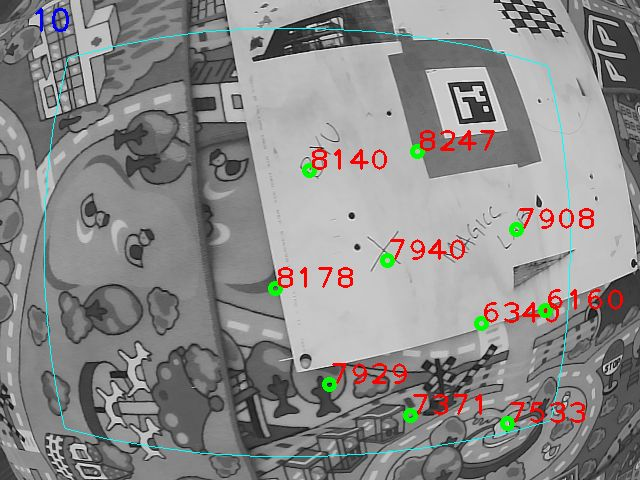
\includegraphics[scale=0.5]{imgs/features_with_aruco.png}
  \caption[Visual Feature Tracking During Flight Experiment]{A processed camera
    image from the multirotor UAV's camera where the landing target vehicle
    occupies the entire image. The ArUco
  marker is pictured in the top, right corner of the image. Each green
circle shows the tracked location of a visual feature used by the
estimator. The red number associated with each visual feature is the unique
integer ID assigned by the feature tracker.}
  \label{fig:features_with_aruco}
\end{figure}

% !TEX root=../root.tex

\subsection{Indoor Motion Capture}
The hardware flight experiments were conducted in the indoor motion capture room
in the MAGICC Lab at Brigham Young University. An Optitrack motion capture
system provided meaurements of the global position and attitude of the UAV
throughout the flights. The motion capture system was also used as ground truth
for the position and attitude of the target vehicle.


% !TEX root=../root.tex

\subsection{Landing Target Vehicle}
As flight tests were conducted in a small indoor environment,
the landing target
vehicle was designed to be small in an attempt to better extend to outdoor
scenarios in which the UAV is to land on larger vehicles such as trucks or boats.
The target vehicle, pictured in~\figref{fig:landing_vehicle}, was manually
driven during the experiments,
roughly following an oval.
% following a rough oval.
% A ground vehicle was assembled as pictured in~\figref{fig:landing_vehicle}
% % with a
% % 6.1 $cm$ ArUco tag serving as the fiducial landing marker.
% % During the experiments, the landing vehicle was
% and manually driven around the
% perimeter of the room during the experiments.

\begin{figure}
  \centering
  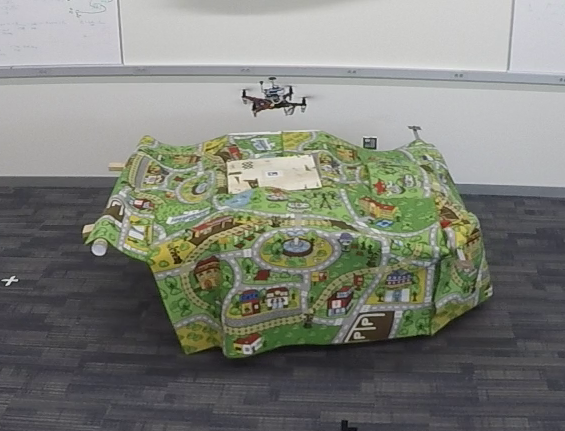
\includegraphics[scale=0.5]{imgs/landing_vehicle.png}
  \caption[UAV Tracking the Target Vehicle During Flight Experiment]{Multirotor
    UAV shown autonomously tracking the landing target
  vehicle.}
  \label{fig:landing_vehicle}
\end{figure}

% !TEX root=../root.tex

\subsection{Experiment Results}
% The multirotor UAV was manually flown until the
% fiducial landing marker was detected. Upon detection, the closed-loop estimation
% and control system took full control of the UAV.

The results of the flight experiment are shown in~\figref{fig:est_hardware}.
The fiducial landing marker was first detected at $t = 20$ s, where the plots
begin.
To demonstrate the ability of the
system to maintain good tracking of a target vehicle when a fiducial
marker is not detected for long periods of time, the fiducial marker detection
was turned off ten seconds after initial detection, at $t = 30$ s.
% The fiducial landing marker was first detected at
% $t = 20$ s and last detected at $t = 30$ s.
It is clear that the estimates of the position, velocity, attitude, and angular
velocity of the target vehicle remained accurate and consistent for the duration
of the experiment.
% despite no measurements from the fiducial marker being used
% after $t = 30$ s.
% Even though no measurements from the fiducial marker are used, it is clear that
% the estimates of the position, velocitity, attitude and angular velocity of the
% target vehicle remain accurate and consistent for the duration of the
% experiment.
These accurate estimates allowed
the UAV to continue to control relative to the target vehicle, tracking closely
above the landing target as the target vehicle moved around the room. After the
target vehicle completed two full laps around the room,
at approximately $t=102$ s, manual control of the UAV was resumed, ending the experiment.
A video of the flight experiment can be found at
\url{https://youtu.be/3AyjCI0c1Nc}.
% \url{https://youtu.be/VU5sq6FuSL0}.

\begin{figure}
  \centering
  \includegraphics[width=6.5in]{plots/hardware_results}
  \caption[ESKF Hardware Results Using Ten Visual Features]{Hardware results when
    the ESKF estimated the positions of \emph{ten} visual
  features. The blue line represents the true state while the orange line
  represents the estimated state. The two grey lines show $\pm 2 \sigma$ bounds for
  the estimate based on the estimated covariance. Measurements from the fiducial
  marker were not used after $t = 30$ s to demonstrate the performance of the estimator.}
  \label{fig:est_hardware}
\end{figure}


\section{Conclusion} \label{sec:conclusion}
The proposed estimator provides a method for maintaining accurate and consistent
estimates of the state of a landing vehicle when a fiducial landing marker is
not detected for significant periods of time. This improvement is achieved by
tracking and estimating the locations of unknown visual features on the landing
vehicle. The simulation and hardware experiments show that by tracking and
estimating the locations of just 10 visual features, the multirotor UAV can
continue to reliably operate with respect to the landing vehicle for long
periods of time without detecting the fiducial landing marker.

% !TEX root=../master.tex

% \chapter{Control Paper}
\chapter{Error-State LQR Control of a Multirotor UAV}
\label{chp:control_paper}

\graphicspath{{lqr_paper/}}

\section{Introduction}
% !TEX root=../root.tex

%\subsection{Background}

Over the past two decades, multirotor unmanned air vehicles (UAVs) have become a
popular platform for robotics research and the base for a variety of consumer and
commercial products. UAVs are currently used all over the world for everything
from military surveillance to package delivery. Larger multirotor vehicles
have even been recently introduced to transport humans. Whatever the
application, multirotors must but able to safely navigate in their environment,
requiring a combination of complex perception, motion planning, and control
algorithms. This paper describes a novel control algorithm that allows a multirotor UAV to
accurately track a desired trajectory in time and space. 

% - UAV control
% - Lie Algebra in estimation Geometric Control
% - Duality to ESKF
% !TEX root=../root.tex

%\subsection{Related Works}

The Linear Quadratic Regulator (LQR) is a well-known feedback controller that
computes the optimal feedback gains for a linear time-invariant (LTI) system
given a quadratic cost function. LQR has been used to control multirotor UAVs with a variety of
approaches. Almost all of these approaches
linearize the system at a given stable state and use a fixed LQR
gain~\cite{cowling2007prototype}. Some have
used a gain scheduling approach with a library of LQR gains for different
magnitudes of deviation from the desired state~\cite{reyes2013lqr}. Recently, an approach was
proposed that relinearizes the system at a fixed rate, slower than the control
loop, and then recomputes the LQR gains at that rate~\cite{foehn2018onboard}. Our
proposed solution takes a similar approach while relinearizing and recomputing
the LQR gains at every control step. 

Recently there has been a movement in the robotics community to appropriately
deal with the evolution of a robot's state along a manifold using Lie
theory~\cite{sola2018micro}. Though these methods have widely been used in the
field of state estimation~\cite{sola2017quaternion,koch2017relative}, a
% field of state estimation~\cite{sola2017quaternion}~\cite{koch2017relative}, a
few methods have emerged that also apply Lie theory to
control~\cite{yu2015high,lee2010geometric}. We propose a formulation of
% control~\cite{yu2015high}~\cite{lee2010geometric}. We propose a formulation of
the LQR problem that properly deals with the manifold nature of the state,
specifically the attitude component. Most previous LQR solutions
for a multirotor UAV use an Euler angle representation of attitude and treat the
tuple of ZYX Euler angles as if it were a vector space~\cite{cowling2007prototype}, even
though it is not~\cite{diebel2006representing}. While some methods use unit
quaternions or rotation matrices to properly represent atttiude, these are also
not inherently a vector space and extra steps are required to orthonormalize or
otherwise force the attitude to stay on the
manifold~\cite{reyes2013lqr,foehn2018onboard}. The proposed solution is
derived from Lie theory and care is taken to ensure that all vector
manipulations are done with
appropriate vector quantities so that the state remains on the manifold.

% \begin{figure}
  % \centering
  % 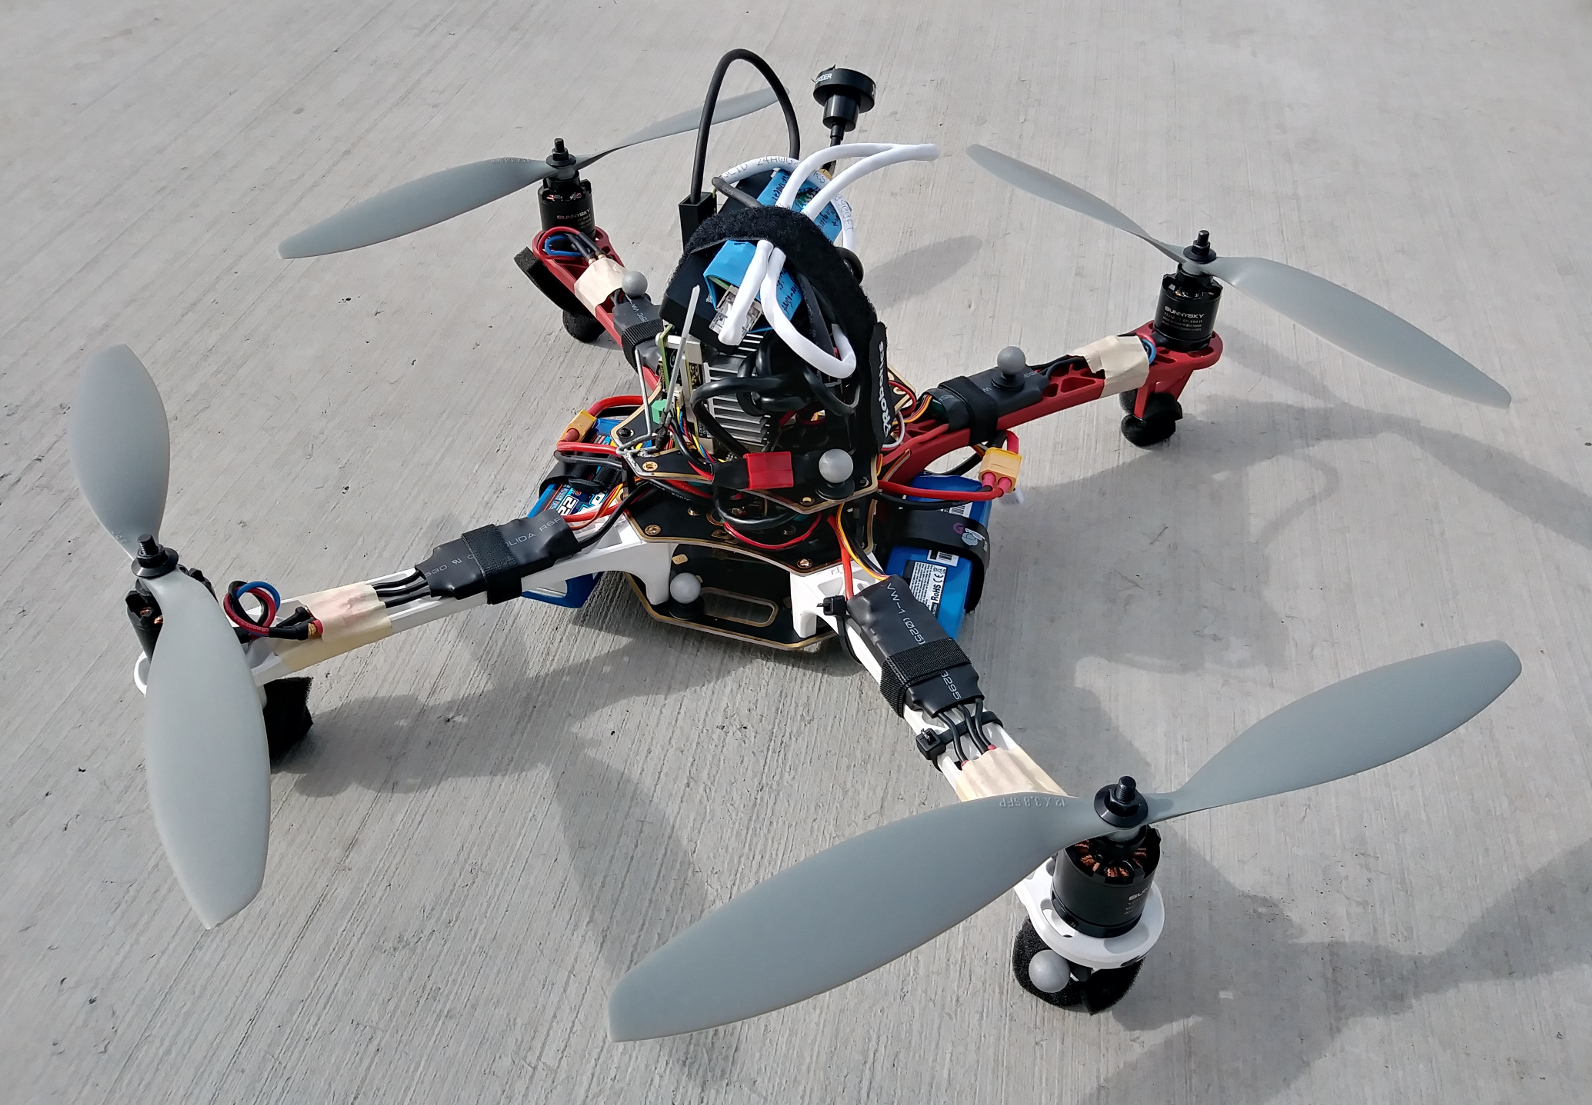
\includegraphics[scale=0.15]{figures/hardware_platform.jpg}
  % \caption[Multirotor UAV Used in Experiments]{Hardware platform used in experiments.}
  % \label{f:drone_pic}
% \end{figure}

% !TEX root=../root.tex

%\subsection{Paper Layout}

\secref{sec:model} explains the multirotor UAV model used in the proposed
controller formulation. \secref{sec:lqr_control} presents traditional LQR
theory and shows how the proposed LQR formulation is a natural extension when
care is taken to apply Lie theory to the multirotor problem.
\secref{sec:experiment} describes the experiments used to demonstrate the
proposed control scheme both in simulation and in hardware.
\secref{sec:results} discusses the results of the experiments and
\secref{sec:conclusion} provides concluding remarks.


\section{Model} \label{sec:model}
% !TEX root=../root.tex

\subsection{Notation}

We define some common notation used throughout the paper, first noting that
vectors are represented with a bold letter (e.g., $\bf v$) and matrices with a
capital letter (e.g., $A$).
\begin{center}
\begin{tabularx}{\columnwidth}{lX}
$R_a^b$ & Rotation matrix from reference frame $a$ to $b$ \\
$\vect{v}_{a/b}^c$ & Vector state $\vect{v}$ of frame $a$ w.r.t.~frame $b$, expressed in frame $c$ \\
% $\hat{a}$ & Estimate of true variable $a$ \\
% $\bar{a}$ & Measurement of $a$ \\
$\des{a}$ & Desired value of $a$ \\
$\dot{a}$ & Time derivative of $a$ \\
$\tilde{a}$ & Error of variable $a$, i.e., $\tilde{a} \triangleq a - \des{a}$
\end{tabularx}
\end{center}
%
We also define the following coordinate frames:
\begin{center}
\begin{tabularx}{\columnwidth}{lX}
$I$ & The inertial coordinate frame in north-east-down\\
$\ell$ & The aircraft's vehicle-1 (body-level) coordinate frame \\
$b$ & The aircraft's body-fixed coordinate frame
\end{tabularx}
\end{center}

We make frequent use of the skew-symmetric matrix operator defined by
\begin{equation}
  \skewmat{\vect{v}} \triangleq
  \begin{bmatrix}
  0 & -v_{3} & v_{2}\\
  v_{3} & 0 & -v_{1}\\
  -v_{2} & v_{1} & 0
  \end{bmatrix},
\end{equation}
which is related to the cross-product between two vectors as
\begin{equation}
  \vect{v}\times\vect{w}=\skewmat{\vect{v}}\vect{w}.
\end{equation}
We also use the standard basis vectors $\vect{e}_1, \vect{e}_2, \ldots, \vect{e}_N$, where $\vect{e}_1 = \begin{bmatrix} 1 & 0 & \cdots & 0 \end{bmatrix}^\transpose$ and so forth.

% !TEX root=../root.tex

\subsection{Quaternion Representation}
\label{appx:quaternions}
A quaternion $\q$ is a hyper-complex number of rank four.  It is well known that
a unit quaternion $\in S^3$ can be used to efficiently represent attitude, as
$S^3$ is a double cover of $\SO(3)$.  Quaternions have the advantage over
$\SO(3)$ of being more efficient to implement on modern hardware~\cite{casey2013AttitudeRepresentation}, therefore in the software implementation of the described algorithm, we use quaternions, rather than rotation matrices.

We use Hamiltonian notation for unit quaternions $\in S^3$
\begin{equation}
\q=\begin{pmatrix}q_{0} & q_{x}i & q_{y} j & q_{z}k \end{pmatrix}%=\begin{pmatrix}q_{0} & \bar{\q} \end{pmatrix},
\end{equation}
and define the complex numbers $i$, $j$, and $k$, such that
\begin{equation}
\begin{array}{rrrcc}
	& & ij &= -ji &= k, \\
	& & jk &= -kj &= i, \\
	& & ki &= -ik &= j, \\
	i^2 &= j^2 &= k^2 & = ijk &= -1.
\end{array}
\end{equation}
For convenience, we sometimes refer to the complex portion of the quaternion as
\begin{equation}
	\bar{\q} = \begin{bmatrix} q_x & q_y & q_z \end{bmatrix} ^\transpose
\end{equation}
and write quaternions as the tuple of the real and complex portions
\begin{equation}
	\q = \begin{pmatrix} q_0 \\ \bar{\q} \end{pmatrix}.
\end{equation}

Given our use of the Hamiltonian notation, the quaternion group operator
$\otimes$ can be written as the following matrix-like product
\begin{equation}
	\q^a \otimes \q^b = \begin{pmatrix} -q_0^a & \left(-\bar{\q}^{a}\right)^\transpose \\ \bar{\q}^a & q^a_0 I + \skewmat{\bar{\q}^a} \end{pmatrix}
	\begin{pmatrix} q^b \\ \bar{\q}^b\end{pmatrix}.
\end{equation}
It is often convenient to convert a quaternion $\q$ to its associated passive rotation matrix.  This is done with
\begin{equation}
\label{eq:R_from_q}
R\left(\q\right)=\left(2q_{0}^{2}-1\right)I-2q_{0}\skewmat{\bar{\q}}+2\bar{\q}\bar{\q}^{\top}\in SO\left(3\right).
\end{equation}

We also need to frequently convert between the Lie group, $S^3$, and the Lie
algebra, $\mathbb{R}^3$, which enables us to operate in a vector space. This is done with the
exponential and logarithmic mappings. The exponential mapping for a unit quaternion is defined as
\begin{align}
\exp_{\q} & :\mathbb{R}^{3}\rightarrow S^3\nonumber \\
\exp_{\q}\left(\vect{\delta}\right) & \triangleq\begin{bmatrix}\cos\left(\frac{\lVert\vect{\delta}\rVert}{2}\right)\\
\sin\left(\frac{\lVert\vect{\delta}\rVert}{2}\right)\frac{\vect{\delta}}{\lVert\vect{\delta}\rVert}
\end{bmatrix},\label{eqn:exponential_map}
\end{align}
with the corresponding logarithmic map defined as
\begin{align}
\log_{\q} & :S^3\rightarrow \mathbb{R}^{3}\nonumber \\
\log_{\q}\left(\q\right) & \triangleq2\;\mathrm{atan2}\left(\left\Vert \bar{\q}\right\Vert ,q_{0}\right)\frac{\bar{\q}}{\left\Vert \bar{\q}\right\Vert }.\label{eqn:log_map}
\end{align}
To avoid numerical issues when $\norm{\vect{\delta}}\approx0$, we also employ the small-angle approximations of the quaternion exponential and logarithm
\begin{align}
\exp_{\q}\left(\vect{\delta}\right) & \approx\begin{bmatrix}1\\
\frac{\vect{\delta}}{2}
\end{bmatrix}\label{eq:quaternion_exp_approx}\\
\log_{\q}\left(\q\right) & \approx2\;\textrm{sign}\left(q_{0}\right)\bar{\q}.\label{eq:quaternion_log_approx}
\end{align}

We also note that rotations may be written equivalently as $\q_a^b=R\left(\q_a^b\right)=R_a^b$, where the choice of these is dictated by convenience.
We use passive rotation matrices, meaning that the rotation matrix $R_a^b$ acts
on a vector $\vect{r}^a$, expressed in frame $a$, and results in the same
vector, now expressed in frame $b$ as
\begin{equation}
\vect{r}^b = R_a^b \vect{r}^a .
\end{equation}

% The $\boxplus$/$\boxminus$ notation for unit quaternions is now defined by
% \begin{align*}
% \boxplus: & S^3\times\mathbb{R}^{3}\rightarrow S^3\\
%  & \q\boxplus\vect{\delta}\triangleq\q\otimes\exp_q\left(\vect{\delta}\right)\\
% \boxminus: & S^3\times S^3\rightarrow\mathbb{R}^{3}\\
%  & \q\boxminus\vect{p}\triangleq\log_q\left(\vect{p}^{-1}\otimes\q\right).
% \end{align*}
% Let's look at one application for clarification.
% With body angular rate $\vect{\omega}_{b/i}^b$, inertial to body rotation $\q_i^b$, and $\vect{\theta}=\vect{\omega}_{b/i}^b \Delta t$, we have
% \begin{align}
% \q_i^b\left(t+\Delta t\right) & =\q_i^b\left(t\right)\boxplus\vect{\theta}\\
% \vect{\theta} & =\q_i^b\left(t+\Delta t\right)\boxminus\q_i^b\left(t\right).
% \end{align}

%\subsection{Quadrotor Dynamics With Quaternion Attitude}
%In the associated software library, we employ the following dynamics for the quadrotor:
%\begin{align}
    %\dot{\vect{p}}_{b/I}^{I} &= 	R\left(\q_{I}^{b}\right)^\transpose \vect{v}_{b/I}^{b} \nonumber \\
	%\dot{\q}_{I}^{b} &= - \frac{1}{2} \begin{pmatrix} 0 \\ \omega_{b/I}^b\end{pmatrix} \otimes \q_I^b\nonumber\\
	%\dot{\vect{v}}_{b/I}^{b} 
	%&= 	g\frac{s}{s_e}\vect{e}_3 + gR\left(\q_I^b\right) \vect{e}_3- \drag\vect{v}_{b/I}^b - \skewmat{\vect{\omega}_{b/I}^b}\vect{v}_{b/I}^b.
	%\label{eq:quat_dynamics}
%\end{align}
%and we solve this using a fourth-order Runge-Kutta extension of \eqref{eq:quaternion_integration}.

% TODO maybe pull from here
%\subsection{Quaternion Error State Dynamics}
%As with the rotation matrix, we wish to find a minimal representation of the error about a quaternion attitude state.  Let us start with the differential equation for quaternion dynamics
%\begin{equation}
	%\dot{\q}_{I}^{b} = \frac{1}{2}\q_I^b \otimes \begin{pmatrix} 0 \\ \vect{\omega}_{b/I}^b\end{pmatrix}.
%\end{equation}
%This can be solved using the quaternion exponential with
%\begin{equation}
	%\q_I^b\left(t\right) = \q_I^b\left(0\right)\otimes\exp_{\q}\left(\int_0^t \vect{\omega}_{b/I}^b\left(\tau\right) d\tau \right).
%\end{equation}
%To reduce this to our minimal vector representation, as we did with rotation matrices in \eqref{eq:att_vector}, let us define the attitude vector $\vect{r}_I^b\left(t\right)=\vect{r}_I^b\left(t_0\right)+\int_{t_0}^t\boldsymbol{\omega}_{b/I}^b\left(\tau\right)d\tau$ with $\vect{r}_I^b\left(t_0\right)=0$ such that
%\begin{equation}
	%\q_I^b\left(t\right) = \q_I^b\left(0\right)\otimes\exp_{\q}\left(\vect{r}_I^b\left(t\right) \right).
%\end{equation}
%It then follows that the error state of our attitude vector is
%\begin{align}
	%\tilde{\vect{r}}_I^{b} 
		%&= \vect{r}_I^b - \hat{\vect{r}}_I^{\hat{b}}  \nonumber \\
		%&= \vect{r}_I^b - R\left(\q_I^b\right) R\left(\q_I^{\hat{b}}\right)^\transpose \hat{\vect{r}}_I^{\hat{b}}\nonumber \\
		%&= \vect{r}_I^b - R\left(\tilde{\q}_{\hat{b}}^b\right)  \hat{\vect{r}}_I^{\hat{b}}
%\end{align}
%and its time derivative is
%\begin{equation}
	%\dot{\tilde{\vect{r}}}_I^{b} = \dot{\vect{r}}_I^b - R\left(\tilde{\q}_{\hat{b}}^b\right)  \dot{\hat{\vect{r}}}_I^{\hat{b}}.
%\end{equation}
%\subsection{Quaternion Trajectory Generation}
%When creating trajectories using differential flatness for quaternion attitude states, the equivalent expression to \eqref{eq:des_attitude} is
%\begin{equation}
	%\des{q}_I^b = \exp_{\q}\left(\vect{e}_3\des{\psi}_{b/I}^I)\right) \otimes \exp_{\q}\left(\theta \vect{\delta}\right) \label{eq:des_attitude}
%\end{equation}
%where, as in \eqref{eq:des_attitude}, $\theta\vect{\delta}$ is the axis-angle error between the desired acceleration and the inertial z-axis.

%% !TEX root=../root.tex

\subsection{Rotations}
\MF{If we use quaternions throughout (because thats part of the point) maybe we
don't need this. But we can take the first talk about passive rotations}

We use passive rotation matrices, meaning that the rotation matrix $R_a^b$ acts on a vector $\vect{r}^a$, expressed in frame $a$, to express it in frame $b$ as
\begin{equation}
\vect{r}^b = R_a^b \vect{r}^a .
\end{equation}
By representing orientation states directly as rotation matrices, as opposed to other representations such as Euler angles or axis-angle, the group structure of the rotation is preserved.
While unit-quaternions also preserve the group structure in a more concise representation, we choose rotation matrices for clarity of presentation in the following derivations.
However, the companion software library implements techniques described in this paper using quaternions, and the mapping between the rotation-matrix and quaternion representations is described in \appxref{appx:quaternions}.

Rotation matrices are elements of the special orthogonal group $\SO(3)$, where the group operator is matrix multiplication.
Incremental changes or perturbations happen in the tangent space.
The tangent space at the identity element $R=I$ is the Lie algebra $\so(3)$.
The exponential and logarithmic mappings map between the group and the algebra:
\begin{align}
\exp &: \so(3) \to \SO(3) \\
\log &: \SO(3) \to \so(3)
\end{align}
For $\SO(3)$ these mappings are the matrix exponential and matrix logarithm.

The Lie algebra is a vector space, and so is isomorphic to $\mathbb{R}^3$.
The hat $^\wedge$ and vee $^\vee$ operators describe this invertible mapping:
\begin{align}
^\wedge &: \mathbb{R}^3 \to \so(3) \\
^\vee &: \so(3) \to \mathbb{R}^3 .
\end{align}
For $\so(3)$ the $^\wedge$ operator is the skew-symmetric operator:
\begin{equation}
^\wedge : \vect{v} \mapsto \skewmat{\vect{v}} ,
\end{equation}
and the $^\vee$ operator is simply the inverse operation.

For convenience in writing differential quantities as vectors in $\mathbb{R}^3$, we define the capitalized exponential and logarithmic mappings as
\begin{align}
\Exp &: \mathbb{R}^3 \to \SO(3) \\
\Exp &: \vect{\omega} \mapsto \exp(\vect{\omega}^\wedge) ,
\end{align}
and
\begin{align}
\Log &: \SO(3) \to \mathbb{R}^3 \\
\Log &: R \mapsto \log(R)^\vee .
\end{align}
For $\SO(3)$, a closed-form solution for the $\Exp$ mapping is given by the Rodriques formula.
These operators are related to the $\boxplus$/$\boxminus$ notation originally described in~\cite{hertzberg2013integrating} as
\begin{align}
R \boxplus \vect{\omega} &\triangleq R \Exp(\vect{\omega}) , \\
R_2 \boxminus R_1 &\triangleq \Log({R_1}^\transpose R_2) .
\end{align}
\DK{Do we want a symbol for the group operator? (e.g. $R_1 \circ R_2$ or $R_1 \cdot R_2$ vs $R_1 R_2$)}

% !TEX root=../root.tex

\subsection{Quadrotor Dynamics}

If we define the state of a quadrotor as the tuple of position, velocity, and
attitude
\begin{equation*}
	%\vect{x} = \begin{pmatrix}\vect{p}_{b/i}^{i}, R_{i}^{b},
        %\vect{v}_{b/i}^{b} \end{pmatrix} \in \mathbb{R}^3 \times \mathbb{R}^3
        %\times S^3
  \vect{x} = \begin{pmatrix}\vect{p}_{b/I}^{I}, \vect{v}_{b/I}^b, \vect{q}_I^{b}
        \end{pmatrix} \in \mathbb{R}^3 \times \mathbb{R}^3
        \times S^3
\end{equation*}
and the input to our system as the tuple of the throttle signal, $s$, and angular
velocity, $\vect{\omega}_{b/I}^b$,
\begin{equation*}
	\vect{u} = \begin{pmatrix}s, \vect{\omega}_{b/i}^b \end{pmatrix} \in
        \mathbb{R}^1 \times \mathbb{R}^3,
\end{equation*}
then the rigid body dynamics of a multirotor UAV are as follows~\cite{leishman2014accel}:
\small
\begin{align}
	% \dot{\vect{x}} &= f\left(\vect{x}, \vect{u}\right) \nonumber \\
	% \begin{pmatrix} 
		\dot{\vect{p}}_{b/I}^{I} &= \left(R_{I}^{b}\right)^\transpose \vect{v}_{b/I}^{b} \nonumber \\
		\dot{\vect{v}}_{b/I}^{b} &= gR_I^b \vect{e}_3 - g\frac{s}{s_e}\vect{e}_3 -
                \drag \left( I - \vect{e}_3 \vect{e}_3^\top \right)
                \vect{v}_{b/I}^b -
                \skewmat{\vect{\omega}_{b/I}^b}\vect{v}_{b/I}^b
                \label{eq:dynamics} \\
                \dot{\vect{q}}_{I}^{b} 
	% \end{pmatrix}
	&= 	
	% \begin{pmatrix} 
		% \left(R_{I}^{b}\right)^\transpose \vect{v}_{b/I}^{b} \\
		% gR_I^b \vect{e}_3 - g\frac{s}{s_e}\vect{e}_3 -
  %               \drag \left( I - \vect{e}_3 \vect{e}_3^\top \right) \vect{v}_{b/I}^b -
  %               \skewmat{\vect{\omega}_{b/I}^b}\vect{v}_{b/I}^b\\
		%-\skewmat{\vect{\omega}_{b/I}^b} R_{I}^{b}
                \q_I^b \otimes \begin{pmatrix} 0 \\ \frac{1}{2}
                \omega_{b/I}^b\end{pmatrix} \nonumber,
	% \end{pmatrix},
\end{align}
\normalsize
where $\drag$ is a linear drag constant, $s_e$ is the throttle command required to hover, and $g$ is the magnitude of gravity.  This model assumes a linear relationship between throttle signal and thrust, which is not always the case.  Although we use this simple model, more sophisticated approaches, such as~\cite{small2018mpc} estimate this relationship online and compensate for it in real time.

%While the differential equation given in~\eqref{eq:dynamics} can be solved in a number of ways, it is important to properly account for
%the manifold nature of the quaternion attitude representation, otherwise the
%integrated attitude will depart from $S^3$.
%and an expensive re-orthonormalization step will be required to ensure the rotation matrix remains member of $\SO(3)$.  A basic zero-order hold integration scheme is given in Appx.~\ref{appx:manifold_integration} where the attitude is integrated on the manifold and a more accurate fourth-order Runga-Kutta method on the manifold is used in the accompanying software library.

\subsection{Error-State Dynamics} \label{subsec:error_state_dyn}

It is useful to consider what is known as the \emph{error state} of the
quadrotor.  This concept has a long history in state estimation and is used in
the error-state Kalman
filter~\cite{sola2017quaternion,Markley2004MultiplicativeVA}.  The error state
is used in state estimation as a principled way to represent the covariance
about attitude in terms of a vector space, as opposed to some local
approximation.  This relationship is also useful in control for the same reason.
Performing control in the vector space of error state provides a principled way
to leverage well-understood and efficient linear algebra machinery to solve
control problems over non-vector quantities, such as attitude.  

We define the error state of some quantity $\vect{y}$ as
\begin{equation}
  \tilde{\vect{y}}=\vect{y} \boxminus \des{\vect{y}},
  \label{eq:error}
\end{equation}
where $\boxminus$ is an appropriate difference operator, as described
by~\cite{hertzberg2013integrating}.  For instance, if $\vect{y}$, 
$\des{\vect{y}}$ $\in \mathbb{R}^{n}$, the $\boxminus$ operator may be
defined as the vector subtraction operator. However, due to the attitude component of our
state, the vector subtraction operator is not defined between $\x$ and
$\des{\x}$. We instead define the
error state piecewise for
each component of the state and combine these into an error-state vector
\begin{equation}
  \tilde{\vect{x}}=\begin{bmatrix}{\tilde{\vect{p}}}_{b/I}^{I} &
  \tilde{\vect{v}}_{b/I}^{b} &
\tilde{\vect{r}}_{I}^{b}\end{bmatrix}^{\top}\in\mathbb{R}^{9\times1},
  \label{eq:error_state}
\end{equation}
where $\tilde{\vect{p}}_{b/I}^{I}$ is the error state associated with
position, $\tilde{\vect{v}}_{b/I}^{b}$ is the error state associated with
velocity, and $\tilde{\vect{r}}_{I}^{b}$ is the error state associated
with attitude.
%While the state itself is a not a vector quantity due to the attitude
%representation, the error state \emph{is} a vector
%quantity, allowing us to use many common techniques to perform control.

In our case, the error states associated with
position and velocity are simply defined using vector subtraction
\begin{align}
  \label{eq:pos_err}
  \tilde{\vect{p}}_{b/I}^{I} &= \vect{p}_{b/I}^{I} - \des{\vect{p}}_{b/I}^{I} \\
  \tilde{\vect{v}}_{b/I}^{b} &= \vect{v}_{b/I}^{b} - \des{\vect{v}}_{b/I}^{b},
  \label{eq:vel_err}
\end{align}
however, the error state associated with attitude is more complicated.
%In simplest terms, the subtraction operator is
%not a sensible operation for a unit quaternion, therefore we must turn to other
%methods to define the error state.

It is commonly understood that any representation of attitude has three
underlying degrees of freedom.  A unit quaternion has four parameters, but its
error can be described in terms of three degrees of freedom that we wish
to represent as a vector quantity.   In a neighborhood sufficiently close to the
identity,
these behave similarly to the Euler angle representation of roll, pitch,
and yaw. However, Euler angles are not a vector because the sequential rotation
method used to define Euler angles nonlinearly couples the three degrees of
freedom. Therefore, we define the vector
\begin{equation}
  \label{eq:r_def}
  \vect{r}_I^b\left(t\right)=\vect{r}_I^b\left(t_0\right)+\int_{t_{0}}^{t}\vect{\omega}_{b/I}^{b}\left(\tau\right)d\tau,
\end{equation}
such that $\vect{r}_I^b\left(t_0\right) = 0$ and $\dot{\vect{r}}_I^b = \vect{\omega}_{b/I}^{b}$.
With this definition, we can use~\eqref{eqn:exponential_map}
and~\eqref{eqn:log_map} to express
\begin{align}
  \label{eq:q_des}
  \q_{I}^{b} &= \des{\q}_{I}^{b} \otimes \exp_{\q} \left(\tilde{\vect{r}}\right) \\
  \tilde{\vect{r}} &= \log_{\q} \left(\left(\des{\q}_{I}^{b}\right)^{-1} \otimes
    \q_{I}^{b}\right),
\end{align}
as described by~\cite{hertzberg2013integrating}.

Even though $\vect{r}_I^b$ is a vector, we cannot simply compute the error state
as $\tilde{\vect{r}}_I^b=\vect{r}_I^b-\des{\vect{r}}_I^b$ because $\vect{r}_I^b$
is a minimal representation of $\vect{q}_I^b$, which is a double cover of the
Lie group $\SO\mathopen{}\mathclose\bgroup\left(3\aftergroup\egroup\right)$. %$SO\left(3\right)$.
Vector subtraction of members in this group is not valid.
However, the derivative of $\vect{r}_I^b$ exists in the tangent space of $\SO\mathopen{}\mathclose\bgroup\left(3\aftergroup\egroup\right)$, so we can perform
\begin{equation}
\label{eq:rdot_diff}
\dot{\tilde{\vect{r}}}_I^b=\dot{\vect{r}}_I^b-R_I^b\left(\des{R}_I^b\right)^{\top}\dot{\des{\vect{r}}}_I^b,
\end{equation}
where $R_I^b\left(\des{R}_I^b\right)^{\top}$ moves the desired vector
derivative, $\dot{\des{\vect{r}}}_I^b$, from its own tangent space to the tangent space of $\dot{\vect{r}}_I^b$.
With both vectors in the same tangent space, the vector subtraction in~\eqref{eq:rdot_diff} is valid.

For use in control, we similarly define an error state for the control input
with the error state being the difference between the current control input and
some reference input.
Using the same definition as in~\eqref{eq:error}, we can see that
\begin{align}
  \tilde{s} &= s - \des{s} \\
  \tilde{\vect{\omega}}_{b/I}^{b} &= \vect{\omega}_{b/I}^{b} - \des{\vect{\omega}}_{b/I}^{b}
  \label{eq:input_error_state}
\end{align}
where $\des{s}$ and $\des{\vect{\omega}}_{b/I}^{b}$ are respectively the reference throttle
signal and reference angular velocity. Note that we do not model the dynamic
response to these inputs. Instead, our model assumes that the multirotor
instantaneously reaches any commanded throttle and angular velocity.

Using the error-state definitions above, we can derive the error-state dynamics
of the quadrotor as
%\begin{equation}
	%\begin{pmatrix} 
                %\dot{\tilde{\vect{p}}}_{b/I}^{I}\\ 
                %\dot{\tilde{\vect{v}}}_{b/I}^{b}\\
                %\dot{\tilde{\vect{q}}}_{I}^{b} 
	%\end{pmatrix}
	%= 	
        %\begin{pmatrix} \left(R_{I}^{b}\right)^\transpose
          %\tilde{\vect{v}}_{b/I}^{b} - \left(R_{I}^{b}\right)^\transpose
          %\skewmat{\vect{v}_{b/I}^{b}} \tilde{\vect{r}}_I^b \\
          %g\skewmat{R_I^b
          %\vect{e}_3} \tilde{\vect{r}}_I^b -g\frac{\tilde{s}}{s_e}\vect{e}_3
          %-\drag \left( I - \vect{e}_3 \vect{e}_3^\transpose \right)
          %\tilde{\vect{v}}_{b/I}^b - \skewmat{\vect{\omega}_{b/I}^b}
          %\tilde{\vect{v}}_{b/I}^b + \skewmat{\vect{v}_{b/I}^b}
          %\tilde{\vect{\omega}}_{b/I}^b \\
          %\tilde{\vect{\omega}}_{b/I}^{b} -
        %\skewmat{\vect{\omega}_{b/I}^{b} } \tilde{\vect{r}}_I^b \end{pmatrix}.
	%\label{eq:error_state_dynamics}
%\end{equation}
\begin{align}
        \dot{\tilde{\vect{p}}}_{b/I}^{I} &= \left(R_{I}^{b}\right)^\transpose
          \tilde{\vect{v}}_{b/I}^{b} - \left(R_{I}^{b}\right)^\transpose
          \skewmat{\vect{v}_{b/I}^{b}} \tilde{\vect{r}}_I^b \nonumber\\
        \dot{\tilde{\vect{v}}}_{b/I}^{b} &= g\skewmat{R_I^b
          \vect{e}_3} \tilde{\vect{r}}_I^b -g\frac{\tilde{s}}{s_e}\vect{e}_3
          -\drag \left( I - \vect{e}_3 \vect{e}_3^\transpose \right)
          \tilde{\vect{v}}_{b/I}^b 
                                         - \skewmat{\vect{\omega}_{b/I}^b}
          \tilde{\vect{v}}_{b/I}^b + \skewmat{\vect{v}_{b/I}^b}
          \tilde{\vect{\omega}}_{b/I}^b 
          \label{eq:error_state_dynamics}
          \\
          % \tilde{\vect{v}}_{b/I}^b \nonumber \\
                                         % & \qquad - \skewmat{\vect{\omega}_{b/I}^b}
          % \tilde{\vect{v}}_{b/I}^b + \skewmat{\vect{v}_{b/I}^b}
          % \tilde{\vect{\omega}}_{b/I}^b \nonumber \\
          \dot{\tilde{\vect{r}}}_{I}^{b} &= \tilde{\vect{\omega}}_{b/I}^{b} -
        \skewmat{\vect{\omega}_{b/I}^{b} } \tilde{\vect{r}}_I^b, \nonumber
\end{align}
or succinctly,
\begin{equation}
  \dot{\tilde{\x}} = f\left(\x, \tilde{\x}, \vect{u}, \tilde{\vect{u}}\right).
\end{equation}
The derivation of these error-state dynamics can be found in
Appendix~\ref{apdx:control_err_state_derivation}.
% The derivation of these error-state dynamics can be found in the following
% section.
% The derivation of these error-state dynamics can be found in the Appendix.


%Therefore, to derive the attitude error state vector
%we begin with the time derivative of a unit quaternion, given by
%\MF{Quaternions not rotation matrix}
%\begin{equation}
  %\dot{R}_I^b = -\skewmat{\boldsymbol{\omega}_{b/I}^b}R_I^b,
%\end{equation}
%which has the well known solution
%\begin{equation}
  %R_I^b\left(t\right) = \exp\left(-\int_{t_0}^t\skewmat{\boldsymbol{\omega}_{b/I}^b\left(\tau\right)d\tau}\right)R_I^b\left(t_0\right).
  %\label{eq:rot_mat_sol}
%\end{equation}
%If we define an \emph{attitude vector} as the three independent degrees of freedom $\vect{r}_I^b\left(t\right)=\vect{r}_I^b\left(t_0\right)+\int_{t_0}^t\boldsymbol{\omega}_{b/I}^b\left(\tau\right)d\tau$ with $\vect{r}_I^b\left(t_0\right)=0$, then we can re-write \eqref{eq:rot_mat_sol} as
%\begin{equation}
  %R_I^b\left(t\right) = \exp\left(-\skewmat{\vect{r}_I^b\left(t\right)}\right)R_I^b\left(t_0\right).
  %\label{eq:att_vector}
%\end{equation}
%and the time derivative of the attitude vector is given by
%\begin{equation}
  %\dot{\vect{r}}_I^b = \boldsymbol{\omega}_{b/I}^b.
%\end{equation}


%We can now define the error state as: \JN{Start directly with the derivative. Attitude is correctly represented on a manifold, so differencing 'attitude vectors' doesn't really make sense.}
%\begin{align}
        %\tilde{\vect{r}}_I^{b} 
                %&= \vect{r}_I^b - \hat{\vect{r}}_I^{\hat{b}}  \nonumber \\
                %&= \vect{r}_I^b - R_{\hat{b}}^b \hat{\vect{r}}_I^{\hat{b}}  \nonumber \\
                %&= \vect{r}_I^b - R_I^{b} \left(R_{I}^{\hat{b}}\right)^\transpose \hat{\vect{r}}_I^{\hat{b}},
        %\label{eq:att_err}
%\end{align}
%and the associated time derivative
%\begin{equation}
  %\dot{\tilde{\vect{r}}}_I^b = \dot{\vect{r}}_I^b - R_{I}^b \left(R_{I}^{\hat{b}}\right)^\transpose \dot{\hat{\vect{r}}}_I^{\hat{b}}.
  %\label{eq:att_err_deriv}
%\end{equation}
%If we define $\tilde{R}_{\hat{b}}^b = R_{I}^b \left(R_{I}^{\hat{b}}\right)^\transpose$, then \eqref{eq:att_err_deriv} becomes
%\begin{equation}
%\dot{\tilde{\vect{r}}}_I^b = \dot{\vect{r}}_I^b -\tilde{R}_{\hat{b}}^b \dot{\hat{\vect{r}}}_I^{\hat{b}}.
%\end{equation}
%The coordinate frame transform in \eqref{eq:att_err} and \eqref{eq:att_err_deriv} arises because the two attitude vectors are expressed in different tangent spaces.  We desire to express our error state in the actual body frame, so we simply move the estimate into that tangent space.



% Dynamics of sim

\section{LQR Control} \label{sec:lqr_control}
% !TEX root=../root.tex

\subsection{Traditional LQR}

A linear-quadratic regulator provides the optimal state space controller gains
for an LTI  system given by
\begin{equation}
\dot{{\bf x}}=A{\bf x}+B{\bf u},
\end{equation}
assuming full-state feedback. We define the cost-to-go for the infinite-time solution as
\begin{equation}
  J(\vect{x},\vect{u})=\int_{0}^{\infty}\left(\vect{x}^{\top}Q\vect{x}+\vect{u}R\vect{u}\right)dt
\label{eq:lqr_cost}
\end{equation}
with $Q$ and $R$ being positive definite matrices that
define the costs associated with the state and the input. The cost function
given in~\eqref{eq:lqr_cost} is minimized by the control input
\begin{equation}
  \vect{u} = -K\vect{x},
\end{equation}
where $K$ is given by
\begin{equation}
  K = R^{-1}B^{\top}P,
\end{equation}
and $P$ is the solution to the Continuous-time Algebraic Riccati Equation (CARE),
\begin{equation}
  A^{\top}P + PA -PBR^{-1}B^{\top}P + Q = 0.
\end{equation}

It should be noted that in its basic form, an LQR controller is simply a
regulator and the control input $\vect{u}$ will only attempt to drive the state
to zero in an optimal way. If the desire is for the system to reach a desired
state, $\des{\vect{x}}$, one can start by defining the error-state as
\begin{equation}
  \tilde{\vect{x}}=\vect{x}-\des{\vect{x}}
  \label{eq:vector_error_state}
\end{equation}
and redefining the control input as
\begin{equation}
  \tilde{\vect{u}} = -K\tilde{\vect{x}}.
\end{equation}
This technique, however, will generally result in steady-state error between the
state $\vect{x}$ and the reference trajectory $\des{\vect{x}}$. The steady-state error can be removed by augmenting the state with an integrator or by applying a model-based feed-forward control input,
\begin{equation}
  \vect{u} = \tilde{\vect{u}} + \des{\vect{u}} = -K\tilde{\vect{x}} + \des{\vect{u}}.
\end{equation}

%In the following sections, we apply an error state LQR controller to
%control the position, velocity, and attitude of a multirotor vehicle. However, a
A direct application of~\eqref{eq:vector_error_state} in our case is not defined
because the multirotor state is not a vector quantity.
%In other words, any attempt
%to directly add or subtract an attitude representation will leave the manifold
To compensate for this, we propose to compute control based
on the error-state dynamics of the system, where the error-state is purely a vector
quantity.

% Brysons rule
% !TEX root=../root.tex

\subsection{Error-State LQR}

We can apply the same LQR approach to the error-state dynamics from
\eqref{eq:error_state_dynamics}. Since LQR control is a regulator, it will drive
the error-state to zero, or our current state to our desired state. Since LQR is
only defined for an LTI system, we can approximate the error-state system as an
LTI system by linearizing about the current state at each time step. This gives
us the system
%Heres the code that implements these
  %A_.setZero();
  %A_.block<3, 3>(dxPOS, dxVEL) = R_I_b.transpose();
  %A_.block<3, 3>(dxPOS, dxATT) = -R_I_b.transpose() * skew_vel;

  %A_.block<3, 3>(dxVEL, dxVEL) = -M - skew_omega;
  %A_.block<3, 3>(dxVEL, dxATT) = skew(R_I_b * grav_vec);

  %A_.block<3, 3>(dxATT, dxATT) = -skew_omega;

  %B_.setZero();
  %B_.block<3, 1>(dxVEL, uTHROTTLE) = -(grav_val_ / hover_throttle_) * e3;
  %B_.block<3, 3>(dxVEL, uOMEGA) = skew_vel;

  %B_.block<3, 3>(dxATT, uOMEGA) = Eigen::Matrix3d::Identity();

\begin{equation}
\dot{\tilde{{\bf x}}}=A\tilde{{\bf x}}+B\tilde{{\bf u}}
\end{equation}
with the matrices $A$ and $B$ given by
\begin{align}
A({\bf x},{\bf u}) & =\frac{\partial}{\partial\tilde{{\bf x}}}f({\bf x},\tilde{{\bf x}},{\bf u},\tilde{{\bf u}})\\
B({\bf x},{\bf u}) & =\frac{\partial}{\partial\tilde{{\bf u}}}f({\bf x},\tilde{{\bf x}},{\bf u},\tilde{{\bf u}}).
\end{align}
Using the error-state dynamics in \eqref{eq:error_state_dynamics} and dropping
the subscripts and superscripts for compactness it can
be seen that
\begin{align}
A({\bf x},{\bf u}) & =\frac{\partial}{\partial\tilde{{\bf x}}}f({\bf x},\tilde{{\bf x}},{\bf u},\tilde{{\bf u}})\\
 & =\begin{bmatrix}{\bf 0} & \frac{\partial\dot{\tilde{{\bf
   p}}}}{\partial\tilde{{\bf v}}} & \frac{\partial\dot{\tilde{{\bf
   p}}}}{\partial\tilde{\vect{r}}} \\[4pt]
{\bf 0} & \frac{\partial\dot{\tilde{{\bf v}}}}{\partial\tilde{{\bf v}}} &
\frac{\partial\dot{\tilde{{\bf v}}}}{\partial\tilde{\vect{r}}} \\[4pt]
{\bf 0} & {\bf 0} & \frac{\partial\dot{\tilde{\vect{r}}}}{\partial\tilde{\vect{r}}}
\end{bmatrix}
\end{align}
with the individual components given by
\begin{align}
  \frac{\partial\dot{\tilde{\vect{p}}}}{\partial\tilde{\vect{v}}} &
  =\left(R_{I}^{b}\right)^\transpose \\
  \frac{\partial\dot{\tilde{\vect{p}}}}{\partial\tilde{\vect{r}}} &
  =-\left(R_{I}^{b}\right)^\transpose \skewmat{\vect{v}_{b/I}^{b}} \\
  \frac{\partial\dot{\tilde{\vect{v}}}}{\partial\tilde{\vect{v}}} & =
-\drag\left(I - \e_3\e_3^\transpose\right) - \skewmat{\vect{\omega}_{b/I}^{b}} \\
  \frac{\partial\dot{\tilde{\vect{v}}}}{\partial\tilde{\vect{r}}} & =
  \skewmat{gR_{I}^{b}\e_3} \\
  \frac{\partial\dot{\tilde{\vect{r}}}}{\partial\tilde{\vect{r}}} & =
  -\skewmat{\vect{\omega}_{b/I}^{b}}.
\end{align}
It can similarly be seen that
\begin{align}
B({\bf x},{\bf u}) & =\frac{\partial}{\partial\tilde{{\bf u}}}f({\bf x},\tilde{{\bf x}},{\bf u},\tilde{{\bf u}})\\
                   & =\begin{bmatrix}{\bf 0} & {\bf 0}\\[4pt]
\frac{\partial\dot{\tilde{{\bf v}}}}{\partial\tilde{s}} & {\bf
\frac{\partial\dot{\tilde{{\bf v}}}}{\partial\tilde{\omega}}}\\[4pt]
{\bf 0} & \frac{\partial\dot{\tilde{\vect{r}}}}{\partial\tilde{\omega}}
\end{bmatrix}
\end{align}
with the individual components given by
\begin{align}
  \frac{\partial\dot{\tilde{\vect{v}}}}{\partial\tilde{s}} & =-\frac{g}{s_e}\e_{3}\\
  \frac{\partial\dot{\tilde{\vect{v}}}}{\partial\tilde{\vect{\omega}}} &
  =\skewmat{{\bf v}_{b/I}^{b}} \\
  \frac{\partial\dot{\tilde{\vect{r}}}}{\partial\tilde{\vect{\omega}}} & =I_{3\times3}.
\end{align}

By linearizing at every time step, the CARE
must be solved at each time step with the current $A$ and $B$ matrices. We use the
closed-form, Schur decomposition method described in~\cite{laub1979schur}. This
method allows us to relinearize and recompute the optimal control at full rate
in our experiments.

Although we relinearize and solve the CARE at each time step, the $Q$ and $R$
weighting matrices are fixed. We choose these gains based on Bryson's
rule~\cite{hespanha2018linear}. In addition, we have found that better results
are achieved by saturating the error-state in accordance with the maximum error
terms used to choose the gains with Bryson's rule.

% Error state dynamics
% assume that we reach commanded omega instant
% Brysons rule
%% !TEX root=../root.tex

\subsection{Schur Solver}


\section{Experiment} \label{sec:experiment}
% !TEX root=../root.tex

To test the proposed error-state LQR controller, we designed two experiments to be
performed in simulation and hardware: (i) tracking step inputs in the desired
position of the UAV and (ii) tracking time-dependent full-state trajectories. We
first explain how we generate these time-dependent trajectories for the
experiments and then detail the experimental setup for both simulation and
hardware.

%dynamically feasible trajectories. For simplicity in trajectory tracking, we use the temporal
%tracking scheme, where the desired state of the multirotor varies with time as
%opposed to the spatial tracking scheme where the multirotor must simply follow a
%trajectory in space~\cite{foehn2018onboard}.

\subsection{Trajectory Generation}
\label{subsec:trajectory_gen}

One important consideration in high-performance control of quadrotors is the
generation of smooth, feasible trajectories.  The quadrotor has the benefit of
being \emph{differentially flat} which means that the required inputs to the
quadrotor can be fully defined using derivatives of the outputs of the system,
the desired position and
heading~\cite{mellinger2011minimum}. If we are given some smooth, differentiable trajectory of our desired
position and heading then we can compute the full state and required inputs as
a function of time
\begin{equation}
	\begin{pmatrix} \des{\vect{p}}_{b/I}^I \left( t \right) \\
	                \des{\q}_I^b \left( t \right) \\
	                \des{\vect{v}}_{b/I}^I \left( t \right) \\
	                \des{s} \left( t \right) \\
	                \des{\vect{\omega}}_{b/I}^I \left( t \right)
	\end{pmatrix} = 
	\des{f} \begin{pmatrix} 
					\des{\vect{p}}_{b/I}^I\left(t\right) \\ 
					\dot{\des{\vect{p}}}_{b/I}^I\left(t\right) \\ 
					\ddot{\des{\vect{p}}}_{b/I}^I\left(t\right) \\ 
					\des{\psi}_{b/I}^I\left(t\right)
					%\dot{\des{\psi}}_{b/I}^I\left(t\right)
	\end{pmatrix}.
\end{equation}
We derive the general case where the desired yaw angle of the multirotor UAV is
a function of time. However, since it is well known that the yaw angle of a multirotor UAV is
easily controllable independent of the other states~\cite{mellinger2011minimum}, we simply command a constant zero yaw in our experiments. 

We now derive the differentially
flat outputs.  First, desired position is given to us directly
\begin{equation}
	\des{\vect{p}}_{b/I}^I = \des{\vect{p}}_{b/I}^I. 
\end{equation}
To derive desired attitude and throttle signal we start 
by applying Newton's second law, and consider the rotation from the heading-rotated, body-level
coordinate frame, $\ell$, to
the body frame, $b$. Note that to avoid the need for an iterative solution, we neglect the forces due to drag
that are accounted for in the quadrotor dynamics in \eqref{eq:dynamics}.
Newton's second law is given by
%force balance is given by
\begin{align}
	\sum F^I &= m\ddot{\des{\vect{p}}}_{b/I}^I\\
    -T \left(\des{R}_\ell^b\right)^\transpose + mg\e_3 &= m\ddot{\des{\vect{p}}}_{b/I}^I\\
    \frac{T}{m}\left(\des{R}_\ell^b\right)^\transpose\e_3 &= g\e_3 -
    \ddot{\des{\vect{p}}}_{b/I}^I.
\end{align}
If we then define $\des{\vect{a}} = g\e_3 - \ddot{\des{\vect{p}}}_{b/I}^I$,
then we get the following expression
\begin{equation}
	\frac{T}{m}\left(\des{R}_\ell^b\right)^\transpose\e_3 = \des{\vect{a}}
\end{equation}
where $T$ and $\des{R}_\ell^b$ must satisfy the following conditions:
\begin{align}
	\frac{T}{m} &= \norm{\des{\vect{a}}} \\
	\quad \des{R}_\ell^I\e_3 &= \frac{\des{\vect{a}}}{\norm{\des{\vect{a}}}}. \label{eq:rot_diff_flat}
\end{align}
Because $T=\tfrac{s}{s_e}gm$, then
\begin{equation}
	\des{s} = \frac{s_e}{g}\norm{\des{\vect{a}}}
\end{equation}
and \eqref{eq:rot_diff_flat} can be solved with
\begin{equation}
	%\des{R}_\ell^b = \exp \left( \skewmat{\theta \vect{\delta}} \right) 
  \des{\q}_\ell^b = \exp_{\q} \left( \theta \vect{\delta} \right)
\end{equation}
where
\begin{align}
  \theta &= \mathrm{cos}^{-1}\left(\vect{e}_3^\transpose\frac{\des{\vect{a}}}{\norm{\des{\vect{a}}}}\right) \\
	\vect{\delta} &= \skewmat{\vect{e}_3}\frac{\des{\vect{a}}}{\norm{\des{\vect{a}}}}.
\end{align}
The heading portion of attitude can now be applied to give us our full desired
attitude
\begin{equation}
	%\des{R}_I^b = \des{R}_\ell^b \exp \left( \skewmat{\des{\psi} \e_3} \right).
  \des{\q}_I^b = \exp_{\q} \left( \des{\psi} \e_3 \right) \otimes \des{\q}_\ell^b.
\end{equation}
Desired velocity can be found using the desired attitude
\begin{equation}
	\des{\vect{v}}_{b/I}^b = \des{R}_I^b \dot{\des{\vect{p}}}_{b/I}^I,
\end{equation}
and the required angular rate is found by taking the time derivative of our desired attitude
\begin{equation}
	\des{\vect{\omega}}_{b/I}^b = \frac{d}{dt} \des{\q}_I^b.
\end{equation}
In our implementation, we do this numerically with central differencing on the manifold.

In summary, the differentially flat output of a quadrotor is given as
follows:
\begin{align}
        \label{eq:traj_p}
	\des{\vect{p}}_{b/I}^I &= \des{\vect{p}}_{b/I}^I \\
	%\des{R}_I^b &= \des{R}_\ell^b \exp \left( \skewmat{\des{\psi} \e_3} \right) \\
	\des{\q}_I^b &= \exp_{\q} \left( \des{\psi} \e_3 \right) \otimes
        \des{\q}_\ell^b \\
	\des{\vect{v}}_{b/I}^b &= \des{R}_I^b \dot{\des{\vect{p}}}_{b/I}^I \\
	\des{s} &= \frac{s_e}{g}\norm{g\e_3 - \ddot{\des{\vect{p}}}_{b/I}^I} \\
	%\des{\vect{\omega}}_{b/I}^b &= \frac{d}{dt} \des{R}_I^b.
	\des{\vect{\omega}}_{b/I}^b &= \frac{d}{dt} \des{\q}_I^b.
        \label{eq:traj_omega}
\end{align}


The examples in this work all reference the same figure-eight trajectory defined by 
\begin{align}
	\des{\vect{p}}_{b/I}^I\left(t\right) &= \vect{p}_{b/I}^I\left(t_0\right)
        + \begin{bmatrix}\delta_x \sin\left(\tfrac{T}{2\pi} t\right) \\[4pt]
        \delta_y \sin\left(\tfrac{T}{\pi} t\right) \\[4pt] \delta_z \sin\left(\tfrac{T}{2\pi} t\right)\end{bmatrix} \\
	\des{\psi}_{b/I}^I\left(t\right) &= 0
	%\des{\psi}_{b/I}^I\left(t\right) &= \psi_{b/I}^I\left(t\right) + \delta_\psi \sin\left(\tfrac{T}{2\pi} t\right)
\end{align}
where the $\delta_{\left(\cdot\right)}$ parameters define the dimensions of the
trajectory, and $T$ defines the period.  While a trajectory defined by periodic
functions is useful for simple demonstrations such as what we perform in this
work, we direct the reader to more sophisticated methods of differentiable
trajectory generation such as~\cite{mellinger2011minimum} for practical application.

% flew waypoints and figure8
% !TEX root=../root.tex

\subsection{Simulation}

For simulation, we used Gazebo\footnote{Gazebo:
\url{www.gazebosim.org}}
% \href{www.gazebosim.org}{www.gazebosim.org}}
and ROS\footnote{Robot Operating System:
\url{www.ros.org}}
% \href{www.ros.org}{www.ros.org}}
with the ROSflight software-in-the-loop
(SIL) simulation~\cite{jackson2016rosflight}. This simulation setup allowed us to test
the exact code that also ran in hardware.



% SIL simulation with Gazebo, ROS
% !TEX root=../root.tex

\subsection{Hardware}

A custom multirotor UAV built on a DJI 450 Flamewheel
frame with an STM32F1 microcontroller running the
ROSflight~\cite{jackson2016rosflight} flight control firmware was flown for the
hardware experiments. The algorithm was
implemented and run in real time onboard on an NVIDIA Jetson
TX2. Though the TX2 has a GPU, all computation is done using only the
ARM CPU, showing that this algorithm can also run at full rate on a variety
of popular onboard computers. The multirotor UAV was flown in a small motion capture room
with feedback from an OptiTrack\footnote{OptiTrack:
\url{www.optitrack.com}}
% \href{www.optitrack.com}{www.optitrack.com}}
motion tracking system. The global position and attitude
measurements from the motion capture system are fused in real time with the
onboard IMU of the UAV using an extended Kalman filter (EKF) to produce
full state estimates. 

For added safety, the computed control inputs are saturated before being sent to
the flight controller. The throttle signal, $s$, was saturated to a maximum
value of 0.85 and the angular rate commands, $\vect{\omega}_{b/I}^b$, were
saturated such that each component $\abs{\omega} \leq 2\,
\nicefrac{\mathrm{rad}}{\mathrm{s}}$.

% Roslfight, TX2

\section{Results} \label{sec:results}
% !TEX root=../root.tex

\subsection{Simulation}

\begin{figure}
  \centering
  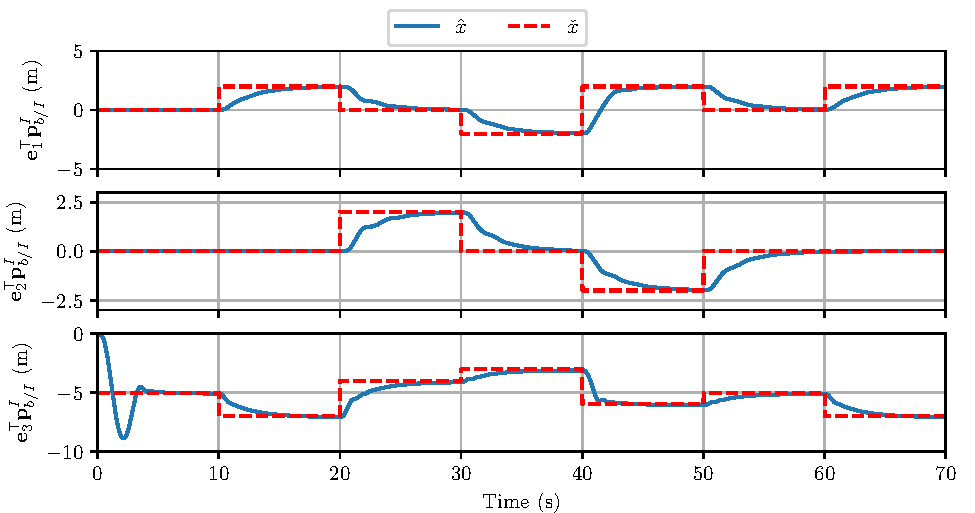
\includegraphics[width=0.6\textwidth]{figures/sim_wps_position}
  \caption[LQR Simulation Results Flying Waypoints]{Simulation results for the position of the multirotor UAV given step
  inputs to position. The red dotted line is the desired position and the blue
solid line is the estimated position.}
  \label{f:sim_wps}
\end{figure}

\begin{figure}
  \centering
  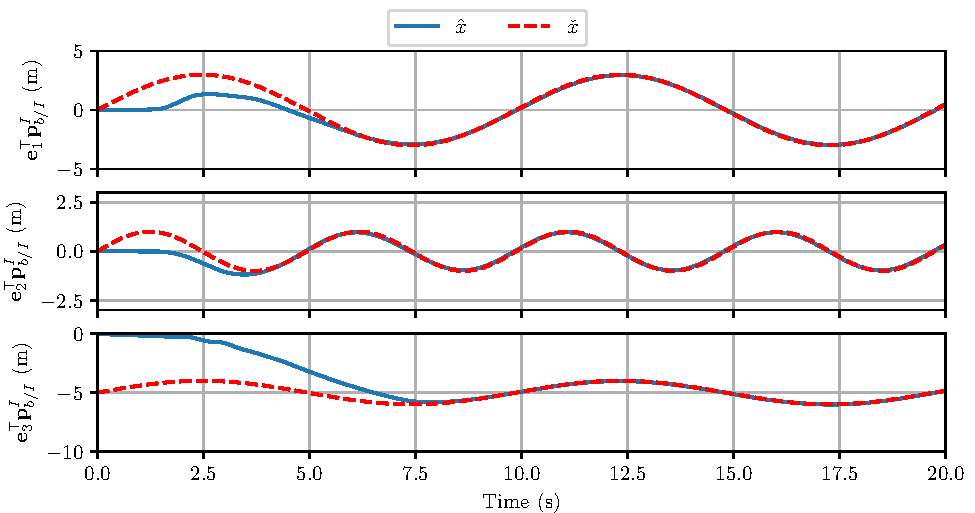
\includegraphics[width=0.6\textwidth]{figures/sim_fig8_position}
  \caption[LQR Simulation Results Flying a Trajectory]{Simulation results of a multirotor UAV tracking a figure eight
  trajectory. The red dotted line is the desired position and the blue solid
line is the estimated position.}
  \label{f:sim_fig8}
\end{figure}

Figs.~\ref{f:sim_wps} and~\ref{f:sim_fig8} show simulation results of the
controller following desired position step inputs (waypoints) and a figure-eight trajectory. The
multirotor begins the simulation at rest on the ground and converges to the
desired trajectory within a few seconds. Note that the figure-eight trajectory
tracking is near perfect even though the feed forward inputs computed
from~\eqref{eq:traj_p}{}--{}~\eqref{eq:traj_omega} do not account for the force due to drag and
the controller does not model thrust dynamics nor torque dynamics.

% !TEX root=../root.tex

\subsection{Hardware}

During the hardware experiments, the entire control algorithm was run at the
full streaming rate of the onboard IMU, which was set to 250 Hz. The computation
time of the algorithm was shown to have a mean of 274.6 $\upmu \mathrm{s}$ and a standard
deviation of 43.84 $\upmu \mathrm{s}$. This shows that the proposed LQR
formulation can run at full rate even on computationally constrained platforms.

\begin{figure}
  \centering
  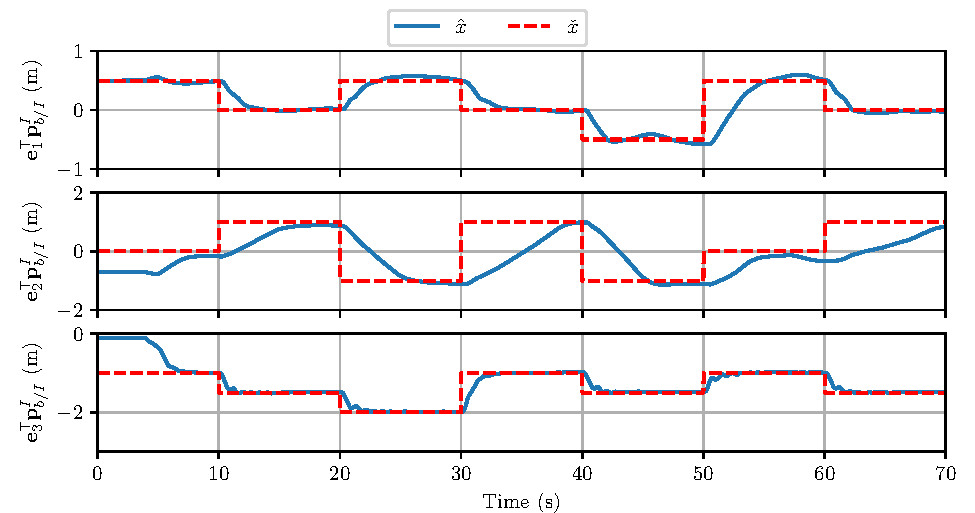
\includegraphics[width=0.4\textwidth]{figures/mocap_wps_position}
  \caption[LQR Hardware Results Flying Waypoints]{Hardware results for the position of the multirotor UAV given step
  inputs to position. The red dotted line is the desired position and the blue
solid line is the estimated position.}
  \label{f:hardware_wps}
\end{figure}

\begin{figure}
  \centering
  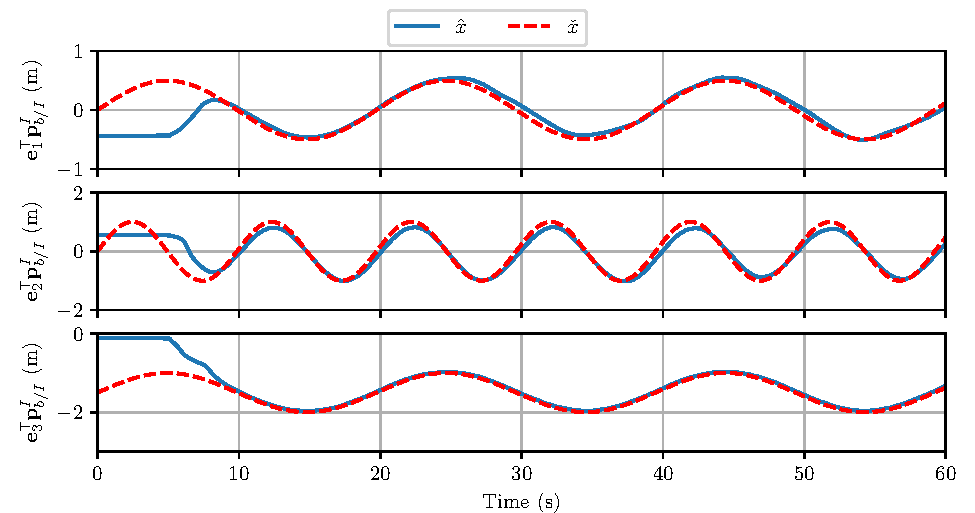
\includegraphics[width=0.4\textwidth]{figures/mocap_fig8_position}
  \caption[LQR Hardware Results Flying a Trajectory]{Hardware results of a multirotor UAV tracking a figure eight
  trajectory. The red dotted line is the desired position and the blue solid
line is the estimated position.}
  \label{f:hardware_fig8}
\end{figure}

\begin{figure}
  \centering
  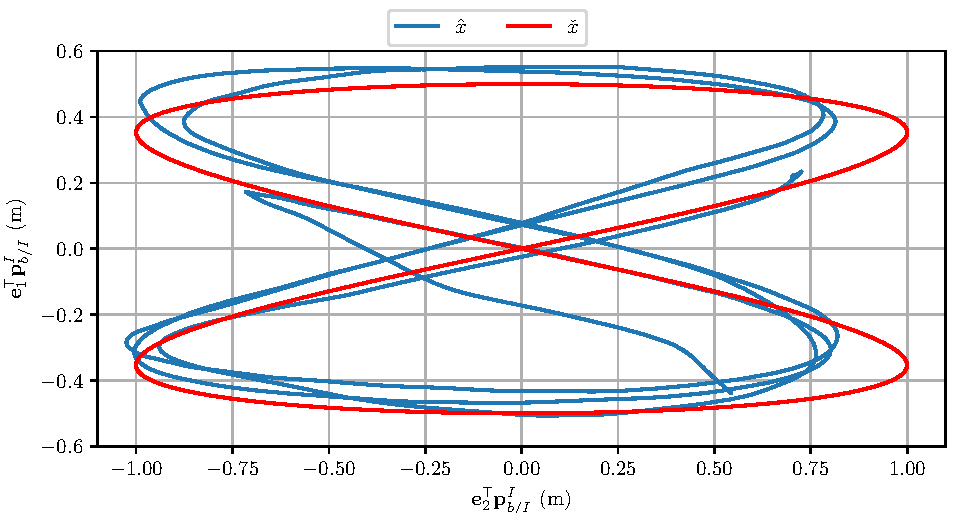
\includegraphics[width=0.4\textwidth]{figures/mocap_fig8_position_2d}
  \caption[Top Down View of LQR Hardware Trajectory]{Top down view of a multirotor UAV tracking a figure eight
  trajectory in hardware. The major deviation in position indicates the time
during take-off when the multirotor must get to the trajectory before following
it. The red solid line is the desired position and the blue solid line is the
estimated position.}
  \label{f:hardware_fig8_2d}
\end{figure}

Fig.~\ref{f:hardware_wps} shows the multirotor position along with the commanded
positions for a waypoint path. The clean step response with minimal overshoot is
notable considering we did not hand tune the LQR gains beyond an initial value
derived from Bryson's rule. Fig. \ref{f:hardware_fig8} shows how well the
multirotor is able to follow the figure-eight trajectory, and Fig.
\ref{f:hardware_fig8_2d} depicts the same flight plotted in two dimensions. The
major deviations visible in this plot depict the take-off and landing portions
of the flight.

% TX2
% 274.6 us mean, 43.84 us std

% Conclusion
\section{Conclusion} \label{sec:conclusion}
% !TEX root=../root.tex

%\subsection{Conclusion}

In this work we propose a novel LQR formulation derived from Lie theory. We
show that by using the error-state dynamics, we can properly compute control
using linear algebra techniques only on appropriate vector quantities. Our implementation is
efficient enough to relinearize the system and update the LQR gains in less than
one millisecond. Simulation and hardware experiments show the effectiveness and
simplicity of this control approach. 



% % What to do about this appendix
% % \appendix
% % \label{app:error_state_der}
% % % !TEX root=../root.tex

To derive the error-state dynamics of the multirotor UAV we first establish a few
identities and approximations. As it is convenient to work with rotation
matrices, we first write~\eqref{eq:q_des} in terms of rotation matrices. Since 
rotation matrices concatenate in an order opposite to quaterions, we have
\begin{equation}
  R_{I}^{b} = R\left(\exp_{\q}\left(\tilde{\vect{r}}_{I}^{b}\right)\right)
  \des{R}_{I}^{b}.
\end{equation}
With this, we can express the desired attitude as
\begin{equation}
  \des{R}_{I}^{b} =
  R\left(\exp_{\q}\left(\tilde{\vect{r}}_{I}^{b}\right)\right)^\transpose R_{I}^{b}.
\end{equation}
and when $\tilde{\vect{r}}_I^b$ is small, we employ~\eqref{eq:quaternion_exp_approx} to get
\begin{align}
  \des{R}_{I}^{b} &\approx R\left(
  \begin{bmatrix}1\\\frac{1}{2}\tilde{\vect{r}}_I^b\end{bmatrix}
\right)^\transpose R_{I}^{b} \\
  \phantom{\des{R}_{I}^{b}} &\approx R\left(
  \begin{bmatrix}1\\-\frac{1}{2}\tilde{\vect{r}}_I^b\end{bmatrix}
\right) R_{I}^{b}.
\end{align}
Now, we can substitute $R\left( \begin{bmatrix}1\\-\frac{1}{2}\tilde{\vect{r}}_I^b\end{bmatrix} \right)$ into eq.~\eqref{eq:R_from_q} to obtain
\begin{equation}
  \des{R}_{I}^{b} \approx \left( I + \skewmat{\tilde{\vect{r}}_I^b} \right)
  R_{I}^{b}.
\end{equation}
We also note that the transpose is given by
\begin{equation}
  \left(\des{R}_{I}^{b}\right)^\transpose =
  \left(R_{I}^{b}\right)^\transpose
  \left(R\left(\exp_{\q}\left(\tilde{\vect{r}}_{I}^{b}\right)\right)\right)
\end{equation}
and can be similarly approximated as
\begin{equation}
  \left(\des{R}_{I}^{b}\right)^\transpose \approx
  \left(R_{I}^{b}\right)^\transpose \left( I - \skewmat{\tilde{\vect{r}}_I^b}
  \right).
\end{equation}
We also employ the skew symmetric identity that
\begin{equation}
  \skewmat{\vect{a}} \vect{b} = -\skewmat{\vect{b}} \vect{a}.
\end{equation}

\subsection{Position}

Differentiating the error state for the position term given
by~\eqref{eq:pos_err} we get
%\begin{align}
%{\bf p}_{b/I}^{I} & =\left({\bf p}_{b/I}^{I}\right)_{\text{ref}}+{\bf \tilde{p}}_{b/I}^{I}\\
%\left({\bf p}_{b/I}^{I}\right)_{\text{ref}} & ={\bf p}_{b/I}^{I}-{\bf \tilde{p}}_{b/I}^{I}\\
%\tilde{{\bf p}}_{b/i}^{i} & ={\bf p}_{b/i}^{i}-\left({\bf p}_{b/i}^{i}\right)_{\text{ref}}.
%\end{align}
%Differentiating we get
\begin{equation}
  \dot{\tilde{\vect{p}}}_{b/I}^{I} = \dot{\vect{p}}_{b/I}^{I} -
    \dot{\des{\vect{p}}}_{b/I}^{I}.
\end{equation}
Substituting in the multirotor dynamics from~\eqref{eq:dynamics} and simplifying
we get
\begin{align}
  \dot{\tilde{\vect{p}}}_{b/I}^{I} &= \left(R_{I}^{b}\right)^\transpose
  \vect{v}_{b/I}^{b} - \left(\des{R}_{I}^{b}\right)^\transpose
  \des{\vect{v}}_{b/I}^{b} \\ 
  &= \left(R_{I}^{b}\right)^\transpose
  \vect{v}_{b/I}^{b} -
  \left(R\left(\exp_{\q}\left(\tilde{\vect{r}}_{I}^{b}\right)\right) R_{I}^{b}\right)^\transpose
  \des{\vect{v}}_{b/I}^{b} \\
  \begin{split}
  &= \left(R_{I}^{b}\right)^\transpose
  \vect{v}_{b/I}^{b}
  - \left(R_{I}^{b}\right)^\transpose
  \left(R\left(\exp_{\q}\left(\tilde{\vect{r}}_{I}^{b}\right)\right) \right)^\transpose
  \left(\vect{v}_{b/I}^{b} - \tilde{\vect{v}}_{b/I}^b\right) \\
  \end{split} \\
  \begin{split}
  &= \left(R_{I}^{b}\right)^\transpose
  \vect{v}_{b/I}^{b}
  - \left(R_{I}^{b}\right)^\transpose
  \left( I - \skewmat{\tilde{\vect{r}}_I^b}\right)
  \left(\vect{v}_{b/I}^{b} - \tilde{\vect{v}}_{b/I}^{b}\right).
  \end{split}
\end{align}
% \begin{align}
  % \dot{\tilde{\vect{p}}}_{b/I}^{I} &= \left(R_{I}^{b}\right)^\transpose
  % \vect{v}_{b/I}^{b} - \left(\des{R}_{I}^{b}\right)^\transpose
  % \des{\vect{v}}_{b/I}^{b} \\ 
  % &= \left(R_{I}^{b}\right)^\transpose
  % \vect{v}_{b/I}^{b} -
  % \left(R\left(\exp_{\q}\left(\tilde{\vect{r}}_{I}^{b}\right)\right) R_{I}^{b}\right)^\transpose
  % \des{\vect{v}}_{b/I}^{b} \\
  % \begin{split}
  % &= \left(R_{I}^{b}\right)^\transpose
  % \vect{v}_{b/I}^{b} \\
  % & \qquad - \left(R_{I}^{b}\right)^\transpose
  % \left(R\left(\exp_{\q}\left(\tilde{\vect{r}}_{I}^{b}\right)\right) \right)^\transpose
  % \left(\vect{v}_{b/I}^{b} - \tilde{\vect{v}}_{b/I}^b\right) \\
  % \end{split} \\
  % \begin{split}
  % &= \left(R_{I}^{b}\right)^\transpose
  % \vect{v}_{b/I}^{b} \\
  % & \qquad - \left(R_{I}^{b}\right)^\transpose
  % \left( I - \skewmat{\tilde{\vect{r}}_I^b}\right)
  % \left(\vect{v}_{b/I}^{b} - \tilde{\vect{v}}_{b/I}^{b}\right).
  % \end{split}
% \end{align}
By simplifying and neglecting higher-order terms, we get the final expression
\begin{equation}
  \dot{\tilde{\vect{p}}}_{b/I}^{I} = \left(R_{I}^{b}\right)^\transpose
  \tilde{\vect{v}}_{b/I}^{b} - \left(R_{I}^{b}\right)^\transpose
    \skewmat{\vect{v}_{b/I}^{b}} \tilde{\vect{r}}_I^b.
\end{equation}

\subsection{Velocity}

Differentiating the error state for the velocity term given
by~\eqref{eq:vel_err} we get
\begin{equation}
  \dot{\tilde{\vect{v}}}_{b/I}^{b} = \dot{\vect{v}}_{b/I}^{b} -
    \dot{\des{\vect{v}}}_{b/I}^{b}.
\end{equation}

Substituting in the multirotor dynamics from~\eqref{eq:dynamics} and simplifying
we get
\begin{align}
\begin{split}
  \dot{\tilde{\vect{v}}}_{b/I}^{b} ={}& \left(gR_I^b \vect{e}_3 -
    g\frac{s}{s_e}\vect{e}_3
    -\drag \left( I - \vect{e}_3 \vect{e}_3^\transpose \right) \vect{v}_{b/I}^b -
                  \skewmat{\vect{\omega}_{b/I}^b}\vect{v}_{b/I}^b\right) \\
    &- \left(g\des{R}_I^b \vect{e}_3 - g\frac{\des{s}}{s_e}\vect{e}_3
    - \drag \left( I - \vect{e}_3 \vect{e}_3^\transpose \right) \des{\vect{v}}_{b/I}^b -
    \skewmat{\des{\vect{\omega}}_{b/I}^b}\des{\vect{v}}_{b/I}^b\right) \\
\end{split} \\
\begin{split}
  \phantom{\dot{\tilde{\vect{v}}}_{b/I}^{b}}={}& \left(gR_I^b \vect{e}_3 -
  g\des{R}_I^b \vect{e}_3\right.) - \left(g\frac{s}{s_e}\vect{e}_3 -
      g\frac{\des{s}}{s_e}\vect{e}_3\right) \\
                                               &-\left(\drag \left( I - \vect{e}_3 \vect{e}_3^\transpose \right)
      \vect{v}_{b/I}^b
    - \drag \left( I - \vect{e}_3 \vect{e}_3^\transpose \right) \des{\vect{v}}_{b/I}^b
    \right) \\
    &- \left(\skewmat{\vect{\omega}_{b/I}^b}\vect{v}_{b/I}^b -
    \skewmat{\des{\vect{\omega}}_{b/I}^b} \des{\vect{v}}_{b/I}^b\right) \\
\end{split} \\
\begin{split}
  \phantom{\dot{\tilde{\vect{v}}}_{b/I}^{b}} \approx {}& \left(gR_I^b \vect{e}_3 -
    g\left( I + \skewmat{\tilde{\vect{r}}_I^b} \right) R_{I}^{b}
  \vect{e}_3\right) \\
    &-\left(g\frac{\tilde{s}}{s_e}\vect{e}_3\right)
    -\left(\drag \left( I - \vect{e}_3 \vect{e}_3^\transpose \right)
    \tilde{\vect{v}}_{b/I}^b\right) \\
    &- \left(\skewmat{\vect{\omega}_{b/I}^b}\vect{v}_{b/I}^b
    -\skewmat{\left(\vect{\omega}_{b/I}^{b} - \tilde{\vect{\omega}}_{b/I}^{b}\right)} 
  \left(\vect{v}_{b/I}^{b} - \tilde{\vect{v}}_{b/I}^{b}\right)\right) \\
\end{split} \\
\begin{split}
  \phantom{\dot{\tilde{\vect{v}}}_{b/I}^{b}} = {}& \left(-g
  \skewmat{\tilde{\vect{r}}_I^b} R_I^b \vect{e}_3\right)
    -\left(g\frac{\tilde{s}}{s_e}\vect{e}_3\right)
    -\left(\drag \left( I - \vect{e}_3 \vect{e}_3^\transpose \right)
    \tilde{\vect{v}}_{b/I}^b\right) \\
    &- \left(\skewmat{\vect{\omega}_{b/I}^b}\vect{v}_{b/I}^b
    -\skewmat{\left(\vect{\omega}_{b/I}^{b} - \tilde{\vect{\omega}}_{b/I}^{b}\right)} 
  \left(\vect{v}_{b/I}^{b} - \tilde{\vect{v}}_{b/I}^{b}\right)\right). \\
\end{split}
\end{align}
% \begin{align}
% \begin{split}
  % \dot{\tilde{\vect{v}}}_{b/I}^{b} ={}& \left(gR_I^b \vect{e}_3 -
    % g\frac{s}{s_e}\vect{e}_3\right. \\
    % &\left.-\drag \left( I - \vect{e}_3 \vect{e}_3^\transpose \right) \vect{v}_{b/I}^b -
                  % \skewmat{\vect{\omega}_{b/I}^b}\vect{v}_{b/I}^b\right) \\
    % &- \left(g\des{R}_I^b \vect{e}_3 - g\frac{\des{s}}{s_e}\vect{e}_3 \right. \\
    % &- \left.\drag \left( I - \vect{e}_3 \vect{e}_3^\transpose \right) \des{\vect{v}}_{b/I}^b -
    % \skewmat{\des{\vect{\omega}}_{b/I}^b}\des{\vect{v}}_{b/I}^b\right) \\
% \end{split} \\
% \begin{split}
  % \phantom{\dot{\tilde{\vect{v}}}_{b/I}^{b}}={}& \left(gR_I^b \vect{e}_3 -
  % g\des{R}_I^b \vect{e}_3\right.) - \left(g\frac{s}{s_e}\vect{e}_3 -
      % g\frac{\des{s}}{s_e}\vect{e}_3\right) \\
    % &-\left(\drag \left( I - \vect{e}_3 \vect{e}_3^\transpose \right)
      % \vect{v}_{b/I}^b\right. \\
    % &- \left.\drag \left( I - \vect{e}_3 \vect{e}_3^\transpose \right) \des{\vect{v}}_{b/I}^b
    % \right) \\
    % &- \left(\skewmat{\vect{\omega}_{b/I}^b}\vect{v}_{b/I}^b -
    % \skewmat{\des{\vect{\omega}}_{b/I}^b} \des{\vect{v}}_{b/I}^b\right) \\
% \end{split} \\
% \begin{split}
  % \phantom{\dot{\tilde{\vect{v}}}_{b/I}^{b}} \approx {}& \left(gR_I^b \vect{e}_3 -
    % g\left( I + \skewmat{\tilde{\vect{r}}_I^b} \right) R_{I}^{b}
  % \vect{e}_3\right) \\
    % &-\left(g\frac{\tilde{s}}{s_e}\vect{e}_3\right)
    % -\left(\drag \left( I - \vect{e}_3 \vect{e}_3^\transpose \right)
    % \tilde{\vect{v}}_{b/I}^b\right) \\
    % &- \left(\skewmat{\vect{\omega}_{b/I}^b}\vect{v}_{b/I}^b\right. \\
    % &-\left.\skewmat{\left(\vect{\omega}_{b/I}^{b} - \tilde{\vect{\omega}}_{b/I}^{b}\right)} 
  % \left(\vect{v}_{b/I}^{b} - \tilde{\vect{v}}_{b/I}^{b}\right)\right) \\
% \end{split} \\
% \begin{split}
  % \phantom{\dot{\tilde{\vect{v}}}_{b/I}^{b}} = {}& \left(-g
  % \skewmat{\tilde{\vect{r}}_I^b} R_I^b \vect{e}_3\right) \\
    % &-\left(g\frac{\tilde{s}}{s_e}\vect{e}_3\right)
    % -\left(\drag \left( I - \vect{e}_3 \vect{e}_3^\transpose \right)
    % \tilde{\vect{v}}_{b/I}^b\right) \\
    % &- \left(\skewmat{\vect{\omega}_{b/I}^b}\vect{v}_{b/I}^b\right. \\
    % &-\left.\skewmat{\left(\vect{\omega}_{b/I}^{b} - \tilde{\vect{\omega}}_{b/I}^{b}\right)} 
  % \left(\vect{v}_{b/I}^{b} - \tilde{\vect{v}}_{b/I}^{b}\right)\right). \\
% \end{split}
% \end{align}

By simplifying and neglecting higher-order terms, we get the final expression
\begin{equation}
  \begin{split}
  \dot{\tilde{\vect{v}}}_{b/I}^{b} = {}& g
  \skewmat{R_I^b \vect{e}_3} \tilde{\vect{r}}_I^b
    -g\frac{\tilde{s}}{s_e}\vect{e}_3
   -\drag \left( I - \vect{e}_3 \vect{e}_3^\transpose \right)
    \tilde{\vect{v}}_{b/I}^b \\
    &- \skewmat{\vect{\omega}_{b/I}^b} \tilde{\vect{v}}_{b/I}^b +
    \skewmat{\vect{v}_{b/I}^b} \tilde{\vect{\omega}}_{b/I}^b.
  \end{split}
\end{equation}
% \begin{equation}
  % \begin{split}
  % \dot{\tilde{\vect{v}}}_{b/I}^{b} = {}& g
  % \skewmat{R_I^b \vect{e}_3} \tilde{\vect{r}}_I^b
    % -g\frac{\tilde{s}}{s_e}\vect{e}_3 \\
    % &-\drag \left( I - \vect{e}_3 \vect{e}_3^\transpose \right)
    % \tilde{\vect{v}}_{b/I}^b \\
    % &- \skewmat{\vect{\omega}_{b/I}^b} \tilde{\vect{v}}_{b/I}^b +
    % \skewmat{\vect{v}_{b/I}^b} \tilde{\vect{\omega}}_{b/I}^b.
  % \end{split}
% \end{equation}

%\begin{multline}
  %\dot{\tilde{\vect{v}}}_{b/I}^{b} =\\
  %\left(gR_I^b \vect{e}_3 - g\frac{s}{s_e}\vect{e}_3 -
%\drag \left( I - \vect{e}_3 \vect{e}_3^\top \right) \vect{v}_{b/I}^b \\
%- \skewmat{\vect{\omega}_{b/I}^b}\vect{v}_{b/I}^b \right) \\
%- \left(gR_I^b \vect{e}_3 - g\frac{s}{s_e}\vect{e}_3 -
%\drag \left( I - \vect{e}_3 \vect{e}_3^\top \right) \vect{v}_{b/I}^b \\
%- \skewmat{\vect{\omega}_{b/I}^b}\vect{v}_{b/I}^b\right)
%\end{multline}

%\begin{align}
%\tilde{{\bf v}}_{b/i}^{b} & ={\bf v}_{b/i}^{b}-\left({\bf v}_{b/i}^{b}\right)_{\text{ref}}\\
 %& =\left(gR_{i}^{b}{\bf e}_{3}-F\frac{g}{F_{\text{hover}}}{\bf e}_{3}-M{\bf v}_{b/i}^{b}-\left({\bf \omega}_{b/i}^{b}\right)^{\wedge}{\bf v}_{b/i}^{b}\right)-\left(gR_{i}^{b}{\bf e}_{3}-F\frac{g}{F_{\text{hover}}}{\bf e}_{3}-M{\bf v}_{b/i}^{b}-\left({\bf \omega}_{b/i}^{b}\right)^{\wedge}{\bf v}_{b/i}^{b}\right)_{\text{ref}}\\
 %& =\left(gR_{i}^{b}{\bf e}_{3}-g\left(R_{i}^{b}\right)_{\text{ref}}{\bf e}_{3}\right)-\left(F\frac{g}{F_{\text{hover}}}{\bf e}_{3}-\left(F\right)_{\text{ref}}\frac{g}{F_{\text{hover}}}{\bf e}_{3}\right)-\left(M{\bf v}_{b/i}^{b}-M\left({\bf v}_{b/i}^{b}\right)_{\text{ref}}\right)-\left(\left({\bf \omega}_{b/i}^{b}\right)^{\wedge}{\bf v}_{b/i}^{b}-\left({\bf \omega}_{b/i}^{b}\right)_{\text{ref}}^{\wedge}\left({\bf v}_{b/i}^{b}\right)_{\text{ref}}\right)\\
 %& =g\left(R_{i}^{b}{\bf e}_{3}-R_{i}^{b}R\left(\exp\left(\tilde{{\bf q}}_{i}^{b}\right)\right){\bf e}_{3}\right)-\left(F\frac{g}{F_{\text{hover}}}{\bf e}_{3}-\left(F-\tilde{F}\right)\frac{g}{F_{\text{hover}}}{\bf e}_{3}\right)-\left(M{\bf v}_{b/i}^{b}-M\left({\bf v}_{b/i}^{b}-{\bf \tilde{v}}_{b/i}^{b}\right)\right)-\left(\left({\bf \omega}_{b/i}^{b}\right)^{\wedge}{\bf v}_{b/i}^{b}-\left({\bf \omega}_{b/i}^{b}-{\bf \tilde{\omega}}_{b/i}^{b}\right)^{\wedge}\left({\bf v}_{b/i}^{b}-{\bf \tilde{v}}_{b/i}^{b}\right)\right)\\
 %& \approx g\left(R_{i}^{b}{\bf e}_{3}-R_{i}^{b}\left(I-\left(\tilde{{\bf q}}_{I}^{b}\right)^{\wedge}\right){\bf e}_{3}\right)-\left(F\frac{g}{F_{\text{hover}}}{\bf e}_{3}-\left(F-\tilde{F}\right)\frac{g}{F_{\text{hover}}}{\bf e}_{3}\right)-\left(M{\bf v}_{b/i}^{b}-M\left({\bf v}_{b/i}^{b}-{\bf \tilde{v}}_{b/i}^{b}\right)\right)-\left(\left({\bf \omega}_{b/i}^{b}\right)^{\wedge}{\bf v}_{b/i}^{b}-\left({\bf \omega}_{b/i}^{b}-{\bf \tilde{\omega}}_{b/i}^{b}\right)^{\wedge}{\bf v}_{b/i}^{b}+\left({\bf \omega}_{b/i}^{b}-{\bf \tilde{\omega}}_{b/i}^{b}\right)^{\wedge}{\bf \tilde{v}}_{b/i}^{b}\right)\\
 %& =g\left(R_{i}^{b}{\bf e}_{3}-R_{i}^{b}{\bf e}_{3}+R_{i}^{b}\left(\tilde{{\bf q}}_{I}^{b}\right)^{\wedge}{\bf e}_{3}\right)-\left(\left(\tilde{F}\right)\frac{g}{F_{\text{hover}}}{\bf e}_{3}\right)-\left(M\left({\bf \tilde{v}}_{b/i}^{b}\right)\right)-\left(\left({\bf \omega}_{b/i}^{b}\right)^{\wedge}{\bf v}_{b/i}^{b}+\left({\bf v}_{b/i}^{b}\right)^{\wedge}\left({\bf \omega}_{b/i}^{b}-{\bf \tilde{\omega}}_{b/i}^{b}\right)-\left({\bf \tilde{v}}_{b/i}^{b}\right)^{\wedge}\left({\bf \omega}_{b/i}^{b}-{\bf \tilde{\omega}}_{b/i}^{b}\right)\right)\\
 %& =g\left(R_{i}^{b}\left(\tilde{{\bf q}}_{I}^{b}\right)^{\wedge}{\bf e}_{3}\right)-\left(\left(\tilde{F}\right)\frac{g}{F_{\text{hover}}}{\bf e}_{3}\right)-\left(M\left({\bf \tilde{v}}_{b/i}^{b}\right)\right)-\left(\left({\bf \omega}_{b/i}^{b}\right)^{\wedge}{\bf v}_{b/i}^{b}+\left({\bf v}_{b/i}^{b}\right)^{\wedge}{\bf \omega}_{b/i}^{b}-\left({\bf v}_{b/i}^{b}\right)^{\wedge}{\bf \tilde{\omega}}_{b/i}^{b}-\left({\bf \tilde{v}}_{b/i}^{b}\right)^{\wedge}{\bf \omega}_{b/i}^{b}+\left({\bf \tilde{v}}_{b/i}^{b}\right)^{\wedge}{\bf \tilde{\omega}}_{b/i}^{b}\right)\\
 %& =g\left(-R_{i}^{b}\left({\bf e}_{3}\right)^{\wedge}\left(\tilde{{\bf q}}_{I}^{b}\right)\right)-\left(\left(\tilde{F}\right)\frac{g}{F_{\text{hover}}}{\bf e}_{3}\right)-\left(M\left({\bf \tilde{v}}_{b/i}^{b}\right)\right)-\left(-\left({\bf v}_{b/i}^{b}\right)^{\wedge}{\bf \tilde{\omega}}_{b/i}^{b}+\left({\bf \omega}_{b/i}^{b}\right)^{\wedge}\left({\bf \tilde{v}}_{b/i}^{b}\right)\right)\\
 %& =-gR_{i}^{b}\left({\bf e}_{3}\right)^{\wedge}\left(\tilde{{\bf q}}_{I}^{b}\right)-\left(\tilde{F}\right)\frac{g}{F_{\text{hover}}}{\bf e}_{3}-M\left({\bf \tilde{v}}_{b/i}^{b}\right)+\left({\bf v}_{b/i}^{b}\right)^{\wedge}{\bf \tilde{\omega}}_{b/i}^{b}-\left({\bf \omega}_{b/i}^{b}\right)^{\wedge}\left({\bf \tilde{v}}_{b/i}^{b}\right)
%\end{align}


\subsection{Attitude}

To derive the error state dynamics corresponding to attitude, we start
with~\eqref{eq:rdot_diff}. From~\eqref{eq:r_def} we see that $\dot{\vect{r}}_I^b
= \vect{\omega}_{b/I}^b$. Substituting this defintion into~\eqref{eq:rdot_diff}
we get
\begin{equation}
\dot{\tilde{\vect{r}}}_I^b = \vect{\omega}_{b/I}^{b} -
R_I^b\left(\des{R}_I^b\right)^\transpose \des{\vect{\omega}}_{b/I}^{b}.
\end{equation}

We can simplify this expression and show that
\begin{align}
  \dot{\tilde{\vect{r}}}_I^b &= \vect{\omega}_{b/I}^{b} -
  R_I^b 
  \left(R_{I}^{b}\right)^\transpose
  \left(R\left(\exp_{\q}\left(\tilde{\vect{r}}_{I}^{b}\right)\right)\right)^\transpose
  \des{\vect{\omega}}_{b/I}^{b} \\
  &\approx \vect{\omega}_{b/I}^{b} -
  R_I^b \left(R_{I}^{b}\right)^\transpose \left( I - \skewmat{\tilde{\vect{r}}_I^b}
  \right) \des{\vect{\omega}}_{b/I}^{b} \\
  &= \vect{\omega}_{b/I}^{b} -
  \left( I - \skewmat{\tilde{\vect{r}}_I^b}
  \right) \left(\vect{\omega}_{b/I}^{b} - \tilde{\vect{\omega}}_{b/I}^{b}\right).
\end{align}
By simplifying and neglecting higher-order terms, we get the final expression
\begin{equation}
  \dot{\tilde{\vect{r}}}_I^b = \tilde{\vect{\omega}}_{b/I}^{b} -
  \skewmat{\vect{\omega}_{b/I}^{b} } \tilde{\vect{r}}_I^b.
\end{equation}


%Using rotation matrices
%\begin{align}
%\dot{R}_{i}^{b} & =R_{i}^{b}\left({\bf \omega}_{b/i}^{b}\right)^{\wedge}\\
%\left(R_{i}^{b}\right)_{\text{ref}} & =R_{I}^{b}R\left(\exp\left(\tilde{{\bf q}}_{I}^{b}\right)\right)
%\end{align}
%Following Sola, we can derive the attitude error state by looking
%at our two different, equivalent expresssions
%\begin{align}
%\dot{{\bf q}}_{i}^{b} & =\frac{1}{2}{\bf q}_{i}^{b}\otimes{\bf \omega}_{b/i}^{b}\\
%{\bf \dot{q}}_{i}^{b} & =\left(\dot{\left({\bf q}_{i}^{b}\right)_{\text{ref}}\otimes\tilde{{\bf q}}_{i}^{b}}\right)
%\end{align}
%With this, we can see that
%\begin{align}
%\left(\dot{\left({\bf q}_{i}^{b}\right)_{\text{ref}}\otimes\tilde{{\bf q}}_{i}^{b}}\right) & =\frac{1}{2}{\bf q}_{i}^{b}\otimes{\bf \omega}_{b/i}^{b}\\
%\left({\bf \dot{q}}_{i}^{b}\right)_{\text{ref}}\otimes\tilde{{\bf q}}_{i}^{b}+\left({\bf q}_{i}^{b}\right)_{\text{ref}}\otimes\dot{\tilde{{\bf q}}}_{i}^{b} & =\frac{1}{2}{\bf q}_{i}^{b}\otimes{\bf \omega}_{b/i}^{b}
%\end{align}
%OR ANOTHER WAY. Though the error state for the attitude term is given
%by 
%\begin{equation}
%\tilde{{\bf q}}_{I}^{b}={\bf q}_{I}^{b}\boxminus\left({\bf q}_{I}^{b}\right)_{\text{ref}}
%\end{equation}
%instead of differentiating through the $\boxminus$ operator, we instead
%use the derivative of attitude in its tanget space. Noting that the
%derivative of the reference attitude and the current attitude lie
%on different tangent spaces, we simply move one onto the other and
%perform regular subtraction because the tangent space is a vector
%space. We have
%\begin{align}
%\tilde{{\bf q}}_{i}^{b} & =\dot{{\bf q}}_{i}^{b}-R_{i}^{b}\left(R_{i}^{b}\right)_{\text{ref}}^{\top}\left({\bf \dot{q}}_{i}^{b}\right)_{\text{ref}}\\
 %& ={\bf \omega}_{b/i}^{b}-\left(R_{i}^{b}\right)\left(R_{i}^{b}\right)_{\text{ref}}^{\top}\left({\bf \omega}_{b/i}^{b}\right)_{\text{ref}}\\
 %& ={\bf \omega}_{b/i}^{b}-\left(R_{i}^{b}\right)\left(R\left(\exp\left(\tilde{{\bf q}}_{I}^{b}\right)\right)R_{I}^{b}\right)^{\top}\left({\bf \omega}_{b/i}^{b}+{\bf \tilde{\omega}}_{b/i}^{b}\right)\\
 %& \approx{\bf \omega}_{b/i}^{b}-\left(R_{i}^{b}\right)\left(R_{I}^{b}\right)^{\top}\left(I+\left(\tilde{{\bf q}}_{I}^{b}\right)^{\wedge}\right)\left({\bf \omega}_{b/i}^{b}+{\bf \tilde{\omega}}_{b/i}^{b}\right)\\
 %& ={\bf \omega}_{b/i}^{b}-\left(I+\left(\tilde{{\bf q}}_{I}^{b}\right)^{\wedge}\right)\left({\bf \omega}_{b/i}^{b}+{\bf \tilde{\omega}}_{b/i}^{b}\right)\\
 %& ={\bf \omega}_{b/i}^{b}-{\bf \omega}_{b/i}^{b}-{\bf \tilde{\omega}}_{b/i}^{b}-\left(\tilde{{\bf q}}_{I}^{b}\right)^{\wedge}{\bf \omega}_{b/i}^{b}-\left(\tilde{{\bf q}}_{I}^{b}\right)^{\wedge}{\bf \tilde{\omega}}_{b/i}^{b}\\
 %& \approx-{\bf \tilde{\omega}}_{b/i}^{b}-\left(\tilde{{\bf q}}_{I}^{b}\right)^{\wedge}{\bf \omega}_{b/i}^{b}\\
 %& =-{\bf \tilde{\omega}}_{b/i}^{b}+\left({\bf \omega}_{b/i}^{b}\right)^{\wedge}\left(\tilde{{\bf q}}_{I}^{b}\right)
%\end{align}




% !TEX root=../master.tex

\chapter{Conclusion}
\label{chp:conclusion}

The robust autonomous operation of multirotor UAVs from moving-vehicle base
stations could benefit a
variety of new industries.
In an effort to make this a possibility,
% The ability of multirotor UAVs to autonomously operate from a moving vehicle
% provides the potential for UAVs to benefit a variety of new industries.
% Working toward this goal,
this
thesis presents improvements to state estimation and control methods used by UAVs
during landing on moving vehicles.
% of a UAV
% for use during landing on a moving vehicle.
The estimation algorithm proposed in
Chapter~\ref{chp:estimation_paper}
allows a UAV to continue to operate reliably with respect to a target vehicle
even when a fiducial landing marker is not detected for significant
periods of time.
The control algorithm proposed in Chapter~\ref{chp:control_paper} provides a principled
and computationally efficient method for a UAV to track a feasible, time-dependent
trajectory.
% to reach touchdown on the target vehicle.
Simulation and hardware tests demonstrated the accurate and robust performance
of these two algorithms.
These results suggest that a reliable system for UAVs landing
on moving vehicles could be developed by combining these proposed state
estimation and control algorithms with an adequate motion planning algorithm.
% The results of simulation and hardware
% experiments show that the combination of these
% % estimation and control
% % algorithms, together with a motion planning algorithm, would result in a robust
% algorithms with a motion planning algorithm would result in a robust
% system for UAVs landing on moving vehicles.

\section{Future Work}
\label{sec:future_work}
While the research in this thesis presents improvements to 
state-of-the-art methods, there remain many opportunities for future
improvements.
The following subsections outline
recommendations and directions for future work related to the autonomous
landing of multirotor UAVs on moving vehicles.
% specific to the fields of state
% estimation, motion planning, and control.
These recommendations are divided into the specific fields of state estimation,
motion planning, and control.

\subsection{State Estimation}
The estimation algorithm presented in Chapter~\ref{chp:estimation_paper} details
a method of tracking and estimating the locations of visual features 
to aid in estimation when a fiducial landing marker is
not detected. The results of this work were quite remarkable, showing that a UAV
can continue to operate accurately with respect to a target vehicle without
detecting a fiducial marker for more
than a minute. However, as mentioned in~\secref{sec:estimation}, this estimation algorithm
assumes that all tracked features are rigidly attached to the target vehicle.
Therefore, before the presented estimation algorithm can be used in a commercial
product, a feature tracker must be developed that can reliably filter out visual
features that are not part of the target vehicle.
Recently, there has been significant research done
in the fields of image and video segmentation that could be leveraged for such a
task~\cite{chen2018encoder}. Alternative methods that depend on
mathematical models of rigid body motion could also be explored as a possible
solution to this problem.

While the proposed estimation method is easily extensible to a variety of
target vehicles, experiments to test this algorithm were only conducted
with a simple ground vehicle.
% testing the estimation
% algorithm with a UAV attempting to land on a ground vehicle which moves on flat
% ground.
In practice, many use cases require UAVs to land on
vehicles with much more complex motion models such as trucks driving on
mountainous terrain or boats on rough seas.
Further experiments should be conducted to test the performance of the presented
estimation algorithm with target vehicles of complex motion models.
% It would be interesting to see if the presented estimation algorithm achieves
% similar levels of success with more complex motion models, or if more
% information about the motion of the landing vehicle is necessary in these cases.
To achieve better results in these scenarios, additional measurement updates
from sensors mounted to the target vehicle, such as GPS or IMU,
could be added  to the algorithm.
% These sensors could include a GPS unit or an
% IMU.
% If more information were necessary, this could easily be done by implementing
% additional measurement updates of
% measurements originating from sensors mounted to the landing vehicle such as a
% GPS unit or an IMU.

\subsection{Motion Planning}
\label{sec:future_motion_planning}
While not discussed in great detail in this thesis, the motion planning problem
associated with multirotor UAVs operating from moving vehicles is 
challenging.
% Motion planning for a UAV also presents a
% problem when the UAV must navigate close to or around obstacles on
% the moving vehicle.
Dynamically feasible trajectories must be planned for UAVs to avoid
obstacles during their approach to the landing target.
This problem is especially important when a UAV must land on a large boat
with significant superstructure or when a UAV must re-enter and land inside of a
package delivery truck. While planning trajectories for UAVs with respect to
static obstacles has been widely researched, planning trajectories to avoid
dynamic obstacles that are rigidly attached to the desired landing target is its
own unique problem to be solved.

When operating from vehicles with complex motion, 
it can also be important to precisely time the touchdown of the UAV.
% potential damage to the UAV.
For instance, when landing on a boat in rough
waters, it may be desireable that the UAV touches down when the heave motion of the
boat reaches a peak to minimize potential damage to the UAV.
% avoid rough contact between the UAV
% and the boat.
Further research should be conducted to plan feasible, time-dependent
trajectories for these scenarios.

% This type of motion planning presents many unsolved challenges.
% While this type of motion planning also requires very detailed
% estimation and prediction of the motion of the boat, the motion
% planning problem itself presents many unsolved challenges.


\subsection{Control}
As discussed in Chapter~\ref{chp:control_paper}, the Lie-theory-based controller
operates on the error state of the system.
% to accurately track a time-dependent trajectory. While
% The main advantage to operating on the error-state
The main advantage to this approach is its mathematically principled nature.
% While operating on the error state provides other
% advantages, the main advantage to this approach is that it is more
% mathematically principled than typical Euler angle formulations.
This, in
theory, allows for more accurate tracking during extreme maneuvers, where
less principled methods, such as typical Euler-angle formulations, struggle.
% extreme maneuvers.
% tracking during extreme maneuvers than less principled methods struggle.
% angle formulations struggle.
% should
% outperform typical Euler angle formulations during extreme maneuvers.
% perform better during more extreme maneuvers than a typical ZYX Euler angle
% formulation.
This controller should be tested with feasible trajectories of acrobatic
maneuvers to demonstrate this advantage.
% Simulation and hardware experiments should be conducted to show the
% advantage this error-state controller presents over existing control schemes.

One key assumption made by the controller is that the
% One potential down side to the proposed controller is that it assumes the
error-state of the system is always small. This was
especially not true in the flight experiments during takeoff, when the UAV was far from the
desired sinusoidal trajectory.
% always true as the UAV had to converge onto the sinusoidal trajectory from stationary
% takeoff.
This resulted in unsteady transient behavior when the error-state values were
not saturated to be small.
% To satisfy this assumption,
% the true performance of the controller,
Instead of a static trajectory,
the controller should be tested with
dynamically planned trajectories which begin at the current state of the
UAV. With these trajectories, the error state of the system would be forced to
be small, satisfying this important assumption.
% small
% always remain small, satisfying the key assumption of the controller.
% The experiments described in~\ref{chp:control_paper} used a simple sinusoidal
% trajectory to demonstrate the performance of the controller. However, the
% transient behavior from take off to convergence onto the trajectory was at times
% unstable. This is a result of the 



%%%%%%%%%%%%% begin Bibliography %%%%%%%%%%%%%%%%%
\cleardoublepage
% \bibliographystyle{asmems4}%Change this to use a different bibliography style, such as ieeetran.
\bibliographystyle{IEEEtran}%Change this to use a different bibliography style, such as ieeetran.
% \bibliography{refs}% Change this to use a different bibliography database file.
\bibliography{abbrev,library}

% Include appendix sections here: (or comment these lines out to have no appendices)
\appendix
\chapter{Derivation of Error-State Dynamics for the Error-State Kalman Filter}
\label{apdx:estimation_err_state_derivation}

\section{UAV Position Error-State Dynamics}
To derive the error-state dynamics for the UAV position state, we start by
differentiating the error-state definition given
in~\eqref{eq:est_paper_uav_pos_err_state} with respect to time to yield
\begin{equation}
  \dot{\tilde{\vect{p}}}_{b/I}^I = \dot{\vect{p}}_{b/I}^I - \dot{\hat{\vect{p}}}_{b/I}^I.
\end{equation}
We then substitue in the corresponding dynamics from~\eqref{eq:uav_dynamics}
and~\eqref{eq:estimated_dynamics}
\begin{align}
  \dot{\tilde{\vect{p}}}_{b/I}^I
  &=
  \left( R_I^b \right)^\transpose \vect{v}_{b/I}^b
  - \left( \hat{R}_I^b \right)^\transpose \hat{\vect{v}}_{b/I}^b.
\end{align}
We expand this equation using the approximation for $\left( R_I^b \right)^\transpose$ given
in~\eqref{eq:est_paper_RTapprox} and the error-state definition given
in~\eqref{eq:est_paper_vector_error_state} resulting in
\begin{align}
  \dot{\tilde{\vect{p}}}_{b/I}^I
  &\approx
  \left( \hat{R}_I^b \right)^\transpose
  \left( I + \skewmat{\tilde{\vect{\theta}}_I^b} \right)
  \left( \hat{\vect{v}}_{b/I}^b + \tilde{\vect{v}}_{b/I}^b \right)
  - \left( \hat{R}_I^b \right)^\transpose \hat{\vect{v}}_{b/I}^b \\
  &\approx
  \left( \hat{R}_I^b \right)^\transpose
  \left( \hat{\vect{v}}_{b/I}^b + \tilde{\vect{v}}_{b/I}^b
  + \skewmat{\tilde{\vect{\theta}}_I^b} \hat{\vect{v}}_{b/I}^b
  + \skewmat{\tilde{\vect{\theta}}_I^b} \tilde{\vect{v}}_{b/I}^b \right)
  - \left( \hat{R}_I^b \right)^\transpose \hat{\vect{v}}_{b/I}^b \\
  &\approx
  \left( \hat{R}_I^b \right)^\transpose \tilde{\vect{v}}_{b/I}^b
  + \left( \hat{R}_I^b \right)^\transpose \skewmat{\tilde{\vect{\theta}}_I^b} \hat{\vect{v}}_{b/I}^b
  + \left( \hat{R}_I^b \right)^\transpose \skewmat{\tilde{\vect{\theta}}_I^b} \tilde{\vect{v}}_{b/I}^b.
\end{align}
We assume the error-state components to be small, neglecting the higher-order
terms to get the final expression
\begin{align}
  \dot{\tilde{\vect{p}}}_{b/I}^I
  &\approx
  \left( \hat{R}_I^b \right)^\transpose \tilde{\vect{v}}_{b/I}^b
  - \left( \hat{R}_I^b \right)^\transpose \skewmat{\hat{\vect{v}}_{b/I}^b}
  \tilde{\vect{\theta}}_I^b.
\end{align}

\section{UAV Attitude Error-State Dynamics}
To derive the error-state dynamics for the UAV attitude state, we
follow~\cite{koch2017relative}, starting
with~\eqref{eq:quat_true_state} and letting $\tilde{\q}_I^b = \exp_{\q} \left(
  \tilde{\vect{\theta}}_I^b \right)$ such that
\begin{equation}
  \q_I^b  = \hat{\q}_I^b \otimes \tilde{\q}_I^b
  \right).
\end{equation}
Differentiating with respect to time results in
\begin{equation}
  \dot{\q}_I^b  = \dot{\hat{\q}}_I^b \otimes \tilde{\q}_I^b + 
  \hat{\q}_I^b \otimes \dot{\tilde{\q}}_I^b
  \right)
\end{equation}
which we multiply all terms on the left by $\left( \hat{\q}_I^b \right)^{-1}$
and simplify to yield
\begin{align}
  \left( \hat{\q}_I^b \right)^{-1} \otimes \dot{\q}_I^b  &= \left( \hat{\q}_I^b
  \right)^{-1} \otimes \dot{\hat{\q}}_I^b \otimes \tilde{\q}_I^b + 
  \left( \hat{\q}_I^b \right)^{-1} \otimes \hat{\q}_I^b \otimes \dot{\tilde{\q}}_I^b
  \right) \\
  \left( \hat{\q}_I^b \right)^{-1} \otimes \dot{\q}_I^b  &= \left( \hat{\q}_I^b
  \right)^{-1} \otimes \dot{\hat{\q}}_I^b \otimes \tilde{\q}_I^b + 
  \dot{\tilde{\q}}_I^b
  \right).
\end{align}
We then rearrange the above equation and simplify using the true-state and
estimated-state dynamics of the UAV attitude state given
in~\eqref{eq:uav_dynamics} and~\eqref{eq:estimated_dynamics} along with the
error-state definition from~\eqref{eq:quat_error_state}:
\begin{align}
  \dot{\tilde{\q}}_I^b &=
  \left( \hat{\q}_I^b \right)^{-1} \otimes \dot{\q}_I^b  - \left( \hat{\q}_I^b
  \right)^{-1} \otimes \dot{\hat{\q}}_I^b \otimes \tilde{\q}_I^b
  \right) \\
  &=
  \left( \hat{\q}_I^b \right)^{-1} \otimes \q_I^b \otimes
  \begin{pmatrix}
    0 \\
    \frac{1}{2} \left( \bar{\vect{\omega}}_{b/I}^b - \vect{\beta}_\omega
    -\vect{\upsilon}_\omega \right)
  \end{pmatrix}
  - \left( \hat{\q}_I^b
  \right)^{-1} \otimes \hat{\q}_I^b \otimes
  \begin{pmatrix}
    0 \\
    \frac{1}{2} \left( \bar{\vect{\omega}}_{b/I}^b - \hat{\vect{\beta}}_\omega
  \end{pmatrix}
  \otimes \tilde{\q}_I^b
  \right) \\
  &=
  \label{eq:intermed_eq1}
  \frac{1}{2} \tilde{\q}_I^b \otimes
  \begin{pmatrix}
    0 \\
    \left( \bar{\vect{\omega}}_{b/I}^b - \vect{\beta}_\omega -
    \vect{\upsilon}_\omega \right)
  \end{pmatrix}
  - \frac{1}{2}
  \begin{pmatrix}
    0 \\
    \left( \bar{\vect{\omega}}_{b/I}^b - \hat{\vect{\beta}}_\omega
  \end{pmatrix}
  \otimes \tilde{\q}_I^b
  \right). 
\end{align}
Applying~\eqref{eq:quat_otimes_product} and noting that the quaternion group
operator $\otimes$ can also be written as
\begin{equation}
	\q^a \otimes \q^b = \begin{pmatrix} q_0^b & \left(-\bar{\q}^{b}\right)^\transpose \\ \bar{\q}^b & q^b_0 I - \skewmat{\bar{\q}^b} \end{pmatrix}
	\begin{pmatrix} q^a \\ \bar{\q}^a \end{pmatrix},
\end{equation}
we can expand~\eqref{eq:intermed_eq1} as matrix-like products
\begin{align}
  \dot{\tilde{\q}}_I^b &=
  \frac{1}{2}
  \begin{pmatrix}
    0 & -\left( \bar{\vect{\omega}}_{b/I}^b - \vect{\beta}_\omega -
      \vect{\upsilon}_\omega
    \right)^\transpose \\
      \left( \bar{\vect{\omega}}_{b/I}^b - \vect{\beta}_\omega -
    \vect{\upsilon}_\omega \right) &
    -\skewmat{\bar{\vect{\omega}}_{b/I}^b - \vect{\beta}_\omega -
    \vect{\upsilon}_\omega }
  \end{pmatrix}
  \tilde{\q}_I^b \\
                       & \qquad - \frac{1}{2}
  \begin{pmatrix}
    0 & -\left( \bar{\vect{\omega}}_{b/I}^b - \hat{\vect{\beta}}_\omega
    \right)^\transpose \\
      \left( \bar{\vect{\omega}}_{b/I}^b - \hat{\vect{\beta}}_\omega \right) &
      \skewmat{\bar{\vect{\omega}}_{b/I}^b - \hat{\vect{\beta}}_\omega }
  \end{pmatrix}
  \tilde{\q}_I^b
  \right). \nonumber
\end{align}
We then simplify the previous equation using the error-state definition
$\tilde{\vect{\beta}}_\omega \triangleq \vect{\beta}_\omega -
\hat{\vect{\beta}}_\omega$ giving
\begin{align}
  \dot{\tilde{\q}}_I^b &=
  \frac{1}{2}
  \begin{pmatrix}
    0 & -\left( - \tilde{\vect{\beta}}_\omega -
      \vect{\upsilon}_\omega
    \right)^\transpose \\
    \left( - \tilde{\vect{\beta}}_\omega -
    \vect{\upsilon}_\omega \right) &
    \skewmat{ -2\bar{\vect{\omega}}_{b/I}^b + 2\hat{\vect{\beta}}_\omega
      + \tilde{\vect{\beta}}_\omega + \vect{\upsilon}_\omega }
  \end{pmatrix}
  \tilde{\q}_I^b
\end{align}
which implies that
\begin{align}
  \begin{pmatrix}
    1 \\
    \frac{1}{2} \dot{\tilde{\vect{\theta}}}_I^b
  \end{pmatrix}
  &=
  \frac{1}{2}
  \begin{pmatrix}
    0 & -\left( - \tilde{\vect{\beta}}_\omega -
      \vect{\upsilon}_\omega
    \right)^\transpose \\
    \left( - \tilde{\vect{\beta}}_\omega -
    \vect{\upsilon}_\omega \right) &
    \skewmat{ -2\bar{\vect{\omega}}_{b/I}^b + 2\hat{\vect{\beta}}_\omega
      + \tilde{\vect{\beta}}_\omega + \vect{\upsilon}_\omega }
  \end{pmatrix}
  \begin{pmatrix}
    1 \\
    \frac{1}{2} \tilde{\vect{\theta}}_I^b
  \end{pmatrix}.
\end{align}
To get the final expression, we drop the scalar equation and neglect
second-order terms to yield
\begin{align}
  \dot{\tilde{\vect{\theta}}}_I^b
  &=
    \left( - \tilde{\vect{\beta}}_\omega -
    \vect{\upsilon}_\omega \right) 
    + \frac{1}{2}
    \skewmat{ -2\bar{\vect{\omega}}_{b/I}^b + 2\hat{\vect{\beta}}_\omega
      + \tilde{\vect{\beta}}_\omega + \vect{\upsilon}_\omega }
    \tilde{\vect{\theta}}_I^b \\
  &\approx
  -\skewmat{ \bar{\vect{\omega}}_{b/I}^b - \hat{\vect{\beta}}_\omega}
    \tilde{\vect{\theta}}_I^b
    - \tilde{\vect{\beta}}_\omega -
    \vect{\upsilon}_\omega .
\end{align}

\section{UAV Velocity Error-State Dynamics}
Similar to the UAV position error-state derivation, to derive the error-state
dynamics for the UAV velocity state, we begin with the time derivative of the
error-state definition
\begin{equation}
  \dot{\tilde{\vect{v}}}_{b/I}^I = \dot{\vect{v}}_{b/I}^I -
  \dot{\hat{\vect{v}}}_{b/I}^I.
\end{equation}
We then substitue in the dynamics from~\eqref{eq:uav_dynamics}
and~\eqref{eq:estimated_dynamics} and expand using the error-state definitions
and approximations
\begin{align}
  \dot{\tilde{\vect{v}}}_{b/I}^I
  =&
  R_I^b \vect{g}
  +
  \skewmat{\vect{v}_{b/I}^b}
  \left( \bar{\vect{\omega}}_{b/I}^b - \vect{\beta}_\omega -
  \vect{\upsilon}_\omega \right)
  +
  \left( \bar{\vect{a}} - \vect{\beta}_a - \vect{\upsilon}_a \right) \\
                                  & \qquad -
                                  \left( \hat{R}_I^b \vect{g}
  +
  \skewmat{\hat{\vect{v}}_{b/I}^b}
  \left( \bar{\vect{\omega}}_{b/I}^b - \hat{\vect{\beta}}_\omega \right)
  +
\left( \bar{\vect{a}} - \hat{\vect{\beta}}_a \right) \right) \nonumber \\
  \approx&
  \left( I - \skewmat{\tilde{\vect{\theta}}_I^b }\right) \hat{R}_I^b \vect{g}
  +
  \skewmat{ \hat{\vect{v}}_{b/I}^b + \tilde{\vect{v}}_{b/I}^b } 
  \left( \bar{\vect{\omega}}_{b/I}^b - \hat{\vect{\beta}}_\omega -
    \tilde{\vect{\beta}}_\omega -
  \vect{\upsilon}_\omega \right) \\
                                  & \qquad 
  + \left( \bar{\vect{a}} - \hat{\vect{\beta}}_a - \tilde{\vect{\beta}}_a - \vect{\upsilon}_a \right)
  - \left( \hat{R}_I^b \vect{g}
  +
  \skewmat{\hat{\vect{v}}_{b/I}^b}
  \left( \bar{\vect{\omega}}_{b/I}^b - \hat{\vect{\beta}}_\omega \right)
  +
\left( \bar{\vect{a}} - \hat{\vect{\beta}}_a \right) \right) \nonumber
\end{align}
which we can simplify and neglect high-order terms to yield the final
expression:
\begin{align}
  \dot{\tilde{\vect{v}}}_{b/I}^I
  \approx&
  \skewmat{ \hat{R}_I^b \vect{g} } \tilde{\vect{\theta}}_I^b 
  -
  \skewmat{ \hat{\vect{v}}_{b/I}^b } \tilde{\vect{\beta}}_\omega
  -
  \skewmat{ \hat{\vect{v}}_{b/I}^b } \vect{\upsilon}_\omega
  -
  \skewmat{ \bar{\omega}_{b/I}^b - \hat{\vect{\beta}}_\omega }
  \tilde{\vect{v}}_{b/I}^b
  -
  \tilde{\vect{\beta}}_a
  -
  \vect{\upsilon}_a.
\end{align}

\section{UAV Bias Error-State Dynamics}
To derive the error-state dynamics for the UAV bias states, we start with the
time derivative of their error-state definitions
\begin{align}
  \dot{\tilde{\vect{\beta}}}_a &= \dot{\vect{\beta}}_a -
  \dot{\hat{\vect{\beta}}}_a \\
  \dot{\tilde{\vect{\beta}}}_\omega &= \dot{\vect{\beta}}_\omega -
  \dot{\hat{\vect{\beta}}}_\omega
\end{align}
We then substitue in the dynamics from~\eqref{eq:uav_dynamics}
and~\eqref{eq:estimated_dynamics} to yield the final expression
\begin{align}
  \dot{\tilde{\vect{\beta}}}_a &= \vect{\eta}_{\beta_a} \\
  \dot{\tilde{\vect{\beta}}}_\omega &= \vect{\eta}_{\beta_\omega}.
\end{align}

\section{Landing Vehicle Position Error-State Dynamics}
Similar to the method used for the UAV states, to derive the error-state
dynamics for the landing vehicle position state, we start with the time
derivative of the error-state definition
\begin{equation}
  \dot{\tilde{\vect{p}}}_{g/b}^{v} = \dot{\vect{p}}_{g/b}^{v} -
  \dot{\hat{\vect{p}}}_{g/b}^{v}.
\end{equation}
We then substitue in the dynamics from~\eqref{eq:goal_dynamics}
and~\eqref{eq:estimated_dynamics} and expand using the error-state definitions
and approximations
\begin{align}
  \dot{\tilde{\vect{p}}}_{g/b}^{v}
  &=
  I_{3 \times 2} \left( R_{I}^{g} \right)^\transpose
  \vect{v}_{g/I}^{g} - \left( R_{I}^{b} \right)^\transpose
  \vect{v}_{b/I}^{b}
  -
  \left(
  I_{3 \times 2} \left( \hat{R}_{I}^{g} \right)^\transpose
  \hat{\vect{v}}_{g/I}^{g} - \left( \hat{R}_{I}^{b} \right)^\transpose
  \hat{\vect{v}}_{b/I}^{b}
  \right) \\
  &\approx
  \label{eq:goal_pos_err_state1}
  I_{3 \times 2} \left( \hat{R}_{I}^{g} \right)^\transpose
  \left( R \left( \tilde{\psi}_{I}^{g} \right) \right)^\transpose
  \left( \hat{\vect{v}}_{g/I}^{g} + \tilde{\vect{v}}_{g/I}^{g} \right) - \left(
  \hat{R}_{I}^{b} \right)^\transpose
  \left( I + \skewmat{\tilde{\vect{\theta}}_I^b} \right)
  \left( \hat{\vect{v}}_{b/I}^{b} + \tilde{\vect{v}}_{b/I}^{b} \right) \\
  & \qquad -
  \left(
  I_{3 \times 2} \left( \hat{R}_{I}^{g} \right)^\transpose
  \hat{\vect{v}}_{g/I}^{g} - \left( \hat{R}_{I}^{b} \right)^\transpose
  \hat{\vect{v}}_{b/I}^{b}
  \right). \nonumber
\end{align}
From~\cite{sola2018micro}, by assuming $\tilde{\psi}_I^g$ is small, we can approximate 
\begin{equation}
  \left( R \left( \tilde{\psi}_I^g \right) \right)^\transpose \approx I -
  \skewmat{\tilde{\psi}_I^g}
  \label{eq:2d_err_rot_approx}
\end{equation}
where the two dimensional skew-symmetric matrix is given by
\begin{equation}
  \skewmat{\psi} \triangleq
  \begin{bmatrix}
    0 & -\psi \\
    \psi & 0
  \end{bmatrix}.
\end{equation}
We can then substitue~\eqref{eq:2d_err_rot_approx}
into~\eqref{eq:goal_pos_err_state1} and simplify and neglect higher-order terms
to get the final expression
\begin{align}
  \dot{\tilde{\vect{p}}}_{g/b}^{v}
  &\approx
  \label{eq:goal_pos_err_state1}
  I_{3 \times 2} \left( \hat{R}_{I}^{g} \right)^\transpose
  \left( I - \skewmat{\tilde{\psi}_I^g} \right)
  \left( \hat{\vect{v}}_{g/I}^{g} + \tilde{\vect{v}}_{g/I}^{g} \right)
  - \left( \hat{R}_{I}^{b} \right)^\transpose
  \left( I + \skewmat{\tilde{\vect{\theta}}_I^b} \right)
  \left( \hat{\vect{v}}_{b/I}^{b} + \tilde{\vect{v}}_{b/I}^{b} \right) \\
  & \qquad -
  \left(
  I_{3 \times 2} \left( \hat{R}_{I}^{g} \right)^\transpose
  \hat{\vect{v}}_{g/I}^{g} - \left( \hat{R}_{I}^{b} \right)^\transpose
  \hat{\vect{v}}_{b/I}^{b}
  \right). \nonumber \\
  &\approx
  \label{eq:goal_pos_err_state1}
  I_{3 \times 2} \left( \hat{R}_{I}^{g} \right)^\transpose
  \tilde{\vect{v}}_{g/I}^g
  +
  I_{3 \times 2} \left( \hat{R}_{I}^{g} \right)^\transpose
  \skewmat{ \tilde{\psi}_I^g } \hat{\vect{v}}_{g/I}^g
  +
  \left( \hat{R}_{I}^{b} \right)^\transpose \skewmat{ \hat{\vect{v}}_{b/I}^{b} } 
  \tilde{\vect{\theta}}_I^b
  -
  \left( \hat{R}_{I}^{b} \right)^\transpose \tilde{\vect{v}}_{b/I}^{b} .
\end{align}

\section{Landing Vehicle Velocity Error-State Dynamics}
Similar to the UAV bias states, the error-state dynamics of the landing vehicle
velocity state are simply found by starting with the time derivative of the
error-state definition
\begin{equation}
  \dot{\tilde{\vect{v}}}_{g/I}^g = \dot{\vect{v}}_{g/I}^g -
  \dot{\hat{\vect{v}}}_{g/I}^g
\end{equation}
and substituting in the dynamics from~\eqref{eq:goal_dynamics}
and~\eqref{eq:estimated_dynamics} to get the final expression
\begin{equation}
  \dot{\tilde{\vect{v}}}_{g/I}^g = \vect{\eta}_{gv}.
\end{equation}

\section{Landing Vehicle Attitude Error-State Dynamics}
\MF{TODO after fix 2D rotation section}

\section{Landing Vehicle Angular Rate Error-State Dynamics}
The error-state dynamics of the landing vehicle angular rate state are found by
starting with the time derivative of the error-state definition
\begin{equation}
  \dot{\tilde{\omega}}_{g/I}^g = \dot{\omega}_{g/I}^g -
  \dot{\hat{\omega}}_{g/I}^g.
\end{equation}
We then substitute in the dynamics from~\eqref{eq:goal_dynamics}
and~\eqref{eq:estimated_dynamics} to yield the final expression
\begin{equation}
  \dot{\tilde{\omega}}_{g/I}^g = \eta_{g\omega}. 
\end{equation}

\section{Visual Feature Vector Error-State Dynamics}
Starting with the time derivative of the error-state definition for the visual
feature vector states,
\begin{equation}
  \dot{\tilde{\vect{r}}}_{i/g}^g = \dot{\vect{r}}_{i/g}^g  -
  \dot{\hat{\vect{r}}}_{i/g}^g,
\end{equation}
and substituting in the dynamics from~\eqref{eq:feature_dynamics}
and~\eqref{eq:estimated_dynamics} yields
\begin{equation}
  \dot{\tilde{\vect{r}}}_{i/g}^g = \vect{0}.
\end{equation}


\chapter{Derivation of Error-State Dynamics for LQR Control}
\label{apdx:control_err_state_derivation}

To derive the error-state dynamics of the multirotor UAV we first establish a few
identities and approximations. As it is convenient to work with rotation
matrices, we first write~\eqref{eq:q_des} in terms of rotation matrices. Since 
rotation matrices concatenate in an order opposite to quaterions, we have
\begin{equation}
  R_{I}^{b} = R\left(\exp_{\q}\left(\tilde{\vect{r}}_{I}^{b}\right)\right)
  \des{R}_{I}^{b}.
\end{equation}
With this, we can express the desired attitude as
\begin{equation}
  \des{R}_{I}^{b} =
  R\left(\exp_{\q}\left(\tilde{\vect{r}}_{I}^{b}\right)\right)^\transpose R_{I}^{b}.
\end{equation}
and when $\tilde{\vect{r}}_I^b$ is small, we employ~\eqref{eq:quaternion_exp_approx} to get
\begin{align}
  \des{R}_{I}^{b} &\approx R\left(
  \begin{bmatrix}1\\\frac{1}{2}\tilde{\vect{r}}_I^b\end{bmatrix}
\right)^\transpose R_{I}^{b} \\
  \phantom{\des{R}_{I}^{b}} &\approx R\left(
  \begin{bmatrix}1\\-\frac{1}{2}\tilde{\vect{r}}_I^b\end{bmatrix}
\right) R_{I}^{b}.
\end{align}
Now, we can substitute $R\left( \begin{bmatrix}1\\-\frac{1}{2}\tilde{\vect{r}}_I^b\end{bmatrix} \right)$ into eq.~\eqref{eq:R_from_q} to obtain
\begin{equation}
  \des{R}_{I}^{b} \approx \left( I + \skewmat{\tilde{\vect{r}}_I^b} \right)
  R_{I}^{b}.
\end{equation}
We also note that the transpose is given by
\begin{equation}
  \left(\des{R}_{I}^{b}\right)^\transpose =
  \left(R_{I}^{b}\right)^\transpose
  \left(R\left(\exp_{\q}\left(\tilde{\vect{r}}_{I}^{b}\right)\right)\right)
\end{equation}
and can be similarly approximated as
\begin{equation}
  \left(\des{R}_{I}^{b}\right)^\transpose \approx
  \left(R_{I}^{b}\right)^\transpose \left( I - \skewmat{\tilde{\vect{r}}_I^b}
  \right).
\end{equation}
We also employ the skew symmetric identity that
\begin{equation}
  \skewmat{\vect{a}} \vect{b} = -\skewmat{\vect{b}} \vect{a}.
\end{equation}

\section{Position}

Differentiating the error state for the position term given
by~\eqref{eq:pos_err} we get
%\begin{align}
%{\bf p}_{b/I}^{I} & =\left({\bf p}_{b/I}^{I}\right)_{\text{ref}}+{\bf \tilde{p}}_{b/I}^{I}\\
%\left({\bf p}_{b/I}^{I}\right)_{\text{ref}} & ={\bf p}_{b/I}^{I}-{\bf \tilde{p}}_{b/I}^{I}\\
%\tilde{{\bf p}}_{b/i}^{i} & ={\bf p}_{b/i}^{i}-\left({\bf p}_{b/i}^{i}\right)_{\text{ref}}.
%\end{align}
%Differentiating we get
\begin{equation}
  \dot{\tilde{\vect{p}}}_{b/I}^{I} = \dot{\vect{p}}_{b/I}^{I} -
    \dot{\des{\vect{p}}}_{b/I}^{I}.
\end{equation}
Substituting in the multirotor dynamics from~\eqref{eq:dynamics} and simplifying
we get
\begin{align}
  \dot{\tilde{\vect{p}}}_{b/I}^{I} &= \left(R_{I}^{b}\right)^\transpose
  \vect{v}_{b/I}^{b} - \left(\des{R}_{I}^{b}\right)^\transpose
  \des{\vect{v}}_{b/I}^{b} \\ 
  &= \left(R_{I}^{b}\right)^\transpose
  \vect{v}_{b/I}^{b} -
  \left(R\left(\exp_{\q}\left(\tilde{\vect{r}}_{I}^{b}\right)\right) R_{I}^{b}\right)^\transpose
  \des{\vect{v}}_{b/I}^{b} \\
  \begin{split}
  &= \left(R_{I}^{b}\right)^\transpose
  \vect{v}_{b/I}^{b}
  - \left(R_{I}^{b}\right)^\transpose
  \left(R\left(\exp_{\q}\left(\tilde{\vect{r}}_{I}^{b}\right)\right) \right)^\transpose
  \left(\vect{v}_{b/I}^{b} - \tilde{\vect{v}}_{b/I}^b\right) \\
  \end{split} \\
  \begin{split}
  &= \left(R_{I}^{b}\right)^\transpose
  \vect{v}_{b/I}^{b}
  - \left(R_{I}^{b}\right)^\transpose
  \left( I - \skewmat{\tilde{\vect{r}}_I^b}\right)
  \left(\vect{v}_{b/I}^{b} - \tilde{\vect{v}}_{b/I}^{b}\right).
  \end{split}
\end{align}
% \begin{align}
  % \dot{\tilde{\vect{p}}}_{b/I}^{I} &= \left(R_{I}^{b}\right)^\transpose
  % \vect{v}_{b/I}^{b} - \left(\des{R}_{I}^{b}\right)^\transpose
  % \des{\vect{v}}_{b/I}^{b} \\ 
  % &= \left(R_{I}^{b}\right)^\transpose
  % \vect{v}_{b/I}^{b} -
  % \left(R\left(\exp_{\q}\left(\tilde{\vect{r}}_{I}^{b}\right)\right) R_{I}^{b}\right)^\transpose
  % \des{\vect{v}}_{b/I}^{b} \\
  % \begin{split}
  % &= \left(R_{I}^{b}\right)^\transpose
  % \vect{v}_{b/I}^{b} \\
  % & \qquad - \left(R_{I}^{b}\right)^\transpose
  % \left(R\left(\exp_{\q}\left(\tilde{\vect{r}}_{I}^{b}\right)\right) \right)^\transpose
  % \left(\vect{v}_{b/I}^{b} - \tilde{\vect{v}}_{b/I}^b\right) \\
  % \end{split} \\
  % \begin{split}
  % &= \left(R_{I}^{b}\right)^\transpose
  % \vect{v}_{b/I}^{b} \\
  % & \qquad - \left(R_{I}^{b}\right)^\transpose
  % \left( I - \skewmat{\tilde{\vect{r}}_I^b}\right)
  % \left(\vect{v}_{b/I}^{b} - \tilde{\vect{v}}_{b/I}^{b}\right).
  % \end{split}
% \end{align}
By simplifying and neglecting higher-order terms, we get the final expression
\begin{equation}
  \dot{\tilde{\vect{p}}}_{b/I}^{I} = \left(R_{I}^{b}\right)^\transpose
  \tilde{\vect{v}}_{b/I}^{b} - \left(R_{I}^{b}\right)^\transpose
    \skewmat{\vect{v}_{b/I}^{b}} \tilde{\vect{r}}_I^b.
\end{equation}

\section{Velocity}

Differentiating the error state for the velocity term given
by~\eqref{eq:vel_err} we get
\begin{equation}
  \dot{\tilde{\vect{v}}}_{b/I}^{b} = \dot{\vect{v}}_{b/I}^{b} -
    \dot{\des{\vect{v}}}_{b/I}^{b}.
\end{equation}

Substituting in the multirotor dynamics from~\eqref{eq:dynamics} and simplifying
we get
\begin{align}
\begin{split}
  \dot{\tilde{\vect{v}}}_{b/I}^{b} ={}& \left(gR_I^b \vect{e}_3 -
    g\frac{s}{s_e}\vect{e}_3
    -\drag \left( I - \vect{e}_3 \vect{e}_3^\transpose \right) \vect{v}_{b/I}^b -
                  \skewmat{\vect{\omega}_{b/I}^b}\vect{v}_{b/I}^b\right) \\
    &- \left(g\des{R}_I^b \vect{e}_3 - g\frac{\des{s}}{s_e}\vect{e}_3
    - \drag \left( I - \vect{e}_3 \vect{e}_3^\transpose \right) \des{\vect{v}}_{b/I}^b -
    \skewmat{\des{\vect{\omega}}_{b/I}^b}\des{\vect{v}}_{b/I}^b\right) \\
\end{split} \\
\begin{split}
  \phantom{\dot{\tilde{\vect{v}}}_{b/I}^{b}}={}& \left(gR_I^b \vect{e}_3 -
  g\des{R}_I^b \vect{e}_3\right.) - \left(g\frac{s}{s_e}\vect{e}_3 -
      g\frac{\des{s}}{s_e}\vect{e}_3\right) \\
                                               &-\left(\drag \left( I - \vect{e}_3 \vect{e}_3^\transpose \right)
      \vect{v}_{b/I}^b
    - \drag \left( I - \vect{e}_3 \vect{e}_3^\transpose \right) \des{\vect{v}}_{b/I}^b
    \right) \\
    &- \left(\skewmat{\vect{\omega}_{b/I}^b}\vect{v}_{b/I}^b -
    \skewmat{\des{\vect{\omega}}_{b/I}^b} \des{\vect{v}}_{b/I}^b\right) \\
\end{split} \\
\begin{split}
  \phantom{\dot{\tilde{\vect{v}}}_{b/I}^{b}} \approx {}& \left(gR_I^b \vect{e}_3 -
    g\left( I + \skewmat{\tilde{\vect{r}}_I^b} \right) R_{I}^{b}
  \vect{e}_3\right) \\
    &-\left(g\frac{\tilde{s}}{s_e}\vect{e}_3\right)
    -\left(\drag \left( I - \vect{e}_3 \vect{e}_3^\transpose \right)
    \tilde{\vect{v}}_{b/I}^b\right) \\
    &- \left(\skewmat{\vect{\omega}_{b/I}^b}\vect{v}_{b/I}^b
    -\skewmat{\left(\vect{\omega}_{b/I}^{b} - \tilde{\vect{\omega}}_{b/I}^{b}\right)} 
  \left(\vect{v}_{b/I}^{b} - \tilde{\vect{v}}_{b/I}^{b}\right)\right) \\
\end{split} \\
\begin{split}
  \phantom{\dot{\tilde{\vect{v}}}_{b/I}^{b}} = {}& \left(-g
  \skewmat{\tilde{\vect{r}}_I^b} R_I^b \vect{e}_3\right)
    -\left(g\frac{\tilde{s}}{s_e}\vect{e}_3\right)
    -\left(\drag \left( I - \vect{e}_3 \vect{e}_3^\transpose \right)
    \tilde{\vect{v}}_{b/I}^b\right) \\
    &- \left(\skewmat{\vect{\omega}_{b/I}^b}\vect{v}_{b/I}^b
    -\skewmat{\left(\vect{\omega}_{b/I}^{b} - \tilde{\vect{\omega}}_{b/I}^{b}\right)} 
  \left(\vect{v}_{b/I}^{b} - \tilde{\vect{v}}_{b/I}^{b}\right)\right). \\
\end{split}
\end{align}
% \begin{align}
% \begin{split}
  % \dot{\tilde{\vect{v}}}_{b/I}^{b} ={}& \left(gR_I^b \vect{e}_3 -
    % g\frac{s}{s_e}\vect{e}_3\right. \\
    % &\left.-\drag \left( I - \vect{e}_3 \vect{e}_3^\transpose \right) \vect{v}_{b/I}^b -
                  % \skewmat{\vect{\omega}_{b/I}^b}\vect{v}_{b/I}^b\right) \\
    % &- \left(g\des{R}_I^b \vect{e}_3 - g\frac{\des{s}}{s_e}\vect{e}_3 \right. \\
    % &- \left.\drag \left( I - \vect{e}_3 \vect{e}_3^\transpose \right) \des{\vect{v}}_{b/I}^b -
    % \skewmat{\des{\vect{\omega}}_{b/I}^b}\des{\vect{v}}_{b/I}^b\right) \\
% \end{split} \\
% \begin{split}
  % \phantom{\dot{\tilde{\vect{v}}}_{b/I}^{b}}={}& \left(gR_I^b \vect{e}_3 -
  % g\des{R}_I^b \vect{e}_3\right.) - \left(g\frac{s}{s_e}\vect{e}_3 -
      % g\frac{\des{s}}{s_e}\vect{e}_3\right) \\
    % &-\left(\drag \left( I - \vect{e}_3 \vect{e}_3^\transpose \right)
      % \vect{v}_{b/I}^b\right. \\
    % &- \left.\drag \left( I - \vect{e}_3 \vect{e}_3^\transpose \right) \des{\vect{v}}_{b/I}^b
    % \right) \\
    % &- \left(\skewmat{\vect{\omega}_{b/I}^b}\vect{v}_{b/I}^b -
    % \skewmat{\des{\vect{\omega}}_{b/I}^b} \des{\vect{v}}_{b/I}^b\right) \\
% \end{split} \\
% \begin{split}
  % \phantom{\dot{\tilde{\vect{v}}}_{b/I}^{b}} \approx {}& \left(gR_I^b \vect{e}_3 -
    % g\left( I + \skewmat{\tilde{\vect{r}}_I^b} \right) R_{I}^{b}
  % \vect{e}_3\right) \\
    % &-\left(g\frac{\tilde{s}}{s_e}\vect{e}_3\right)
    % -\left(\drag \left( I - \vect{e}_3 \vect{e}_3^\transpose \right)
    % \tilde{\vect{v}}_{b/I}^b\right) \\
    % &- \left(\skewmat{\vect{\omega}_{b/I}^b}\vect{v}_{b/I}^b\right. \\
    % &-\left.\skewmat{\left(\vect{\omega}_{b/I}^{b} - \tilde{\vect{\omega}}_{b/I}^{b}\right)} 
  % \left(\vect{v}_{b/I}^{b} - \tilde{\vect{v}}_{b/I}^{b}\right)\right) \\
% \end{split} \\
% \begin{split}
  % \phantom{\dot{\tilde{\vect{v}}}_{b/I}^{b}} = {}& \left(-g
  % \skewmat{\tilde{\vect{r}}_I^b} R_I^b \vect{e}_3\right) \\
    % &-\left(g\frac{\tilde{s}}{s_e}\vect{e}_3\right)
    % -\left(\drag \left( I - \vect{e}_3 \vect{e}_3^\transpose \right)
    % \tilde{\vect{v}}_{b/I}^b\right) \\
    % &- \left(\skewmat{\vect{\omega}_{b/I}^b}\vect{v}_{b/I}^b\right. \\
    % &-\left.\skewmat{\left(\vect{\omega}_{b/I}^{b} - \tilde{\vect{\omega}}_{b/I}^{b}\right)} 
  % \left(\vect{v}_{b/I}^{b} - \tilde{\vect{v}}_{b/I}^{b}\right)\right). \\
% \end{split}
% \end{align}

By simplifying and neglecting higher-order terms, we get the final expression
\begin{equation}
  \begin{split}
  \dot{\tilde{\vect{v}}}_{b/I}^{b} = {}& g
  \skewmat{R_I^b \vect{e}_3} \tilde{\vect{r}}_I^b
    -g\frac{\tilde{s}}{s_e}\vect{e}_3
   -\drag \left( I - \vect{e}_3 \vect{e}_3^\transpose \right)
    \tilde{\vect{v}}_{b/I}^b \\
    &- \skewmat{\vect{\omega}_{b/I}^b} \tilde{\vect{v}}_{b/I}^b +
    \skewmat{\vect{v}_{b/I}^b} \tilde{\vect{\omega}}_{b/I}^b.
  \end{split}
\end{equation}
% \begin{equation}
  % \begin{split}
  % \dot{\tilde{\vect{v}}}_{b/I}^{b} = {}& g
  % \skewmat{R_I^b \vect{e}_3} \tilde{\vect{r}}_I^b
    % -g\frac{\tilde{s}}{s_e}\vect{e}_3 \\
    % &-\drag \left( I - \vect{e}_3 \vect{e}_3^\transpose \right)
    % \tilde{\vect{v}}_{b/I}^b \\
    % &- \skewmat{\vect{\omega}_{b/I}^b} \tilde{\vect{v}}_{b/I}^b +
    % \skewmat{\vect{v}_{b/I}^b} \tilde{\vect{\omega}}_{b/I}^b.
  % \end{split}
% \end{equation}

%\begin{multline}
  %\dot{\tilde{\vect{v}}}_{b/I}^{b} =\\
  %\left(gR_I^b \vect{e}_3 - g\frac{s}{s_e}\vect{e}_3 -
%\drag \left( I - \vect{e}_3 \vect{e}_3^\top \right) \vect{v}_{b/I}^b \\
%- \skewmat{\vect{\omega}_{b/I}^b}\vect{v}_{b/I}^b \right) \\
%- \left(gR_I^b \vect{e}_3 - g\frac{s}{s_e}\vect{e}_3 -
%\drag \left( I - \vect{e}_3 \vect{e}_3^\top \right) \vect{v}_{b/I}^b \\
%- \skewmat{\vect{\omega}_{b/I}^b}\vect{v}_{b/I}^b\right)
%\end{multline}

%\begin{align}
%\tilde{{\bf v}}_{b/i}^{b} & ={\bf v}_{b/i}^{b}-\left({\bf v}_{b/i}^{b}\right)_{\text{ref}}\\
 %& =\left(gR_{i}^{b}{\bf e}_{3}-F\frac{g}{F_{\text{hover}}}{\bf e}_{3}-M{\bf v}_{b/i}^{b}-\left({\bf \omega}_{b/i}^{b}\right)^{\wedge}{\bf v}_{b/i}^{b}\right)-\left(gR_{i}^{b}{\bf e}_{3}-F\frac{g}{F_{\text{hover}}}{\bf e}_{3}-M{\bf v}_{b/i}^{b}-\left({\bf \omega}_{b/i}^{b}\right)^{\wedge}{\bf v}_{b/i}^{b}\right)_{\text{ref}}\\
 %& =\left(gR_{i}^{b}{\bf e}_{3}-g\left(R_{i}^{b}\right)_{\text{ref}}{\bf e}_{3}\right)-\left(F\frac{g}{F_{\text{hover}}}{\bf e}_{3}-\left(F\right)_{\text{ref}}\frac{g}{F_{\text{hover}}}{\bf e}_{3}\right)-\left(M{\bf v}_{b/i}^{b}-M\left({\bf v}_{b/i}^{b}\right)_{\text{ref}}\right)-\left(\left({\bf \omega}_{b/i}^{b}\right)^{\wedge}{\bf v}_{b/i}^{b}-\left({\bf \omega}_{b/i}^{b}\right)_{\text{ref}}^{\wedge}\left({\bf v}_{b/i}^{b}\right)_{\text{ref}}\right)\\
 %& =g\left(R_{i}^{b}{\bf e}_{3}-R_{i}^{b}R\left(\exp\left(\tilde{{\bf q}}_{i}^{b}\right)\right){\bf e}_{3}\right)-\left(F\frac{g}{F_{\text{hover}}}{\bf e}_{3}-\left(F-\tilde{F}\right)\frac{g}{F_{\text{hover}}}{\bf e}_{3}\right)-\left(M{\bf v}_{b/i}^{b}-M\left({\bf v}_{b/i}^{b}-{\bf \tilde{v}}_{b/i}^{b}\right)\right)-\left(\left({\bf \omega}_{b/i}^{b}\right)^{\wedge}{\bf v}_{b/i}^{b}-\left({\bf \omega}_{b/i}^{b}-{\bf \tilde{\omega}}_{b/i}^{b}\right)^{\wedge}\left({\bf v}_{b/i}^{b}-{\bf \tilde{v}}_{b/i}^{b}\right)\right)\\
 %& \approx g\left(R_{i}^{b}{\bf e}_{3}-R_{i}^{b}\left(I-\left(\tilde{{\bf q}}_{I}^{b}\right)^{\wedge}\right){\bf e}_{3}\right)-\left(F\frac{g}{F_{\text{hover}}}{\bf e}_{3}-\left(F-\tilde{F}\right)\frac{g}{F_{\text{hover}}}{\bf e}_{3}\right)-\left(M{\bf v}_{b/i}^{b}-M\left({\bf v}_{b/i}^{b}-{\bf \tilde{v}}_{b/i}^{b}\right)\right)-\left(\left({\bf \omega}_{b/i}^{b}\right)^{\wedge}{\bf v}_{b/i}^{b}-\left({\bf \omega}_{b/i}^{b}-{\bf \tilde{\omega}}_{b/i}^{b}\right)^{\wedge}{\bf v}_{b/i}^{b}+\left({\bf \omega}_{b/i}^{b}-{\bf \tilde{\omega}}_{b/i}^{b}\right)^{\wedge}{\bf \tilde{v}}_{b/i}^{b}\right)\\
 %& =g\left(R_{i}^{b}{\bf e}_{3}-R_{i}^{b}{\bf e}_{3}+R_{i}^{b}\left(\tilde{{\bf q}}_{I}^{b}\right)^{\wedge}{\bf e}_{3}\right)-\left(\left(\tilde{F}\right)\frac{g}{F_{\text{hover}}}{\bf e}_{3}\right)-\left(M\left({\bf \tilde{v}}_{b/i}^{b}\right)\right)-\left(\left({\bf \omega}_{b/i}^{b}\right)^{\wedge}{\bf v}_{b/i}^{b}+\left({\bf v}_{b/i}^{b}\right)^{\wedge}\left({\bf \omega}_{b/i}^{b}-{\bf \tilde{\omega}}_{b/i}^{b}\right)-\left({\bf \tilde{v}}_{b/i}^{b}\right)^{\wedge}\left({\bf \omega}_{b/i}^{b}-{\bf \tilde{\omega}}_{b/i}^{b}\right)\right)\\
 %& =g\left(R_{i}^{b}\left(\tilde{{\bf q}}_{I}^{b}\right)^{\wedge}{\bf e}_{3}\right)-\left(\left(\tilde{F}\right)\frac{g}{F_{\text{hover}}}{\bf e}_{3}\right)-\left(M\left({\bf \tilde{v}}_{b/i}^{b}\right)\right)-\left(\left({\bf \omega}_{b/i}^{b}\right)^{\wedge}{\bf v}_{b/i}^{b}+\left({\bf v}_{b/i}^{b}\right)^{\wedge}{\bf \omega}_{b/i}^{b}-\left({\bf v}_{b/i}^{b}\right)^{\wedge}{\bf \tilde{\omega}}_{b/i}^{b}-\left({\bf \tilde{v}}_{b/i}^{b}\right)^{\wedge}{\bf \omega}_{b/i}^{b}+\left({\bf \tilde{v}}_{b/i}^{b}\right)^{\wedge}{\bf \tilde{\omega}}_{b/i}^{b}\right)\\
 %& =g\left(-R_{i}^{b}\left({\bf e}_{3}\right)^{\wedge}\left(\tilde{{\bf q}}_{I}^{b}\right)\right)-\left(\left(\tilde{F}\right)\frac{g}{F_{\text{hover}}}{\bf e}_{3}\right)-\left(M\left({\bf \tilde{v}}_{b/i}^{b}\right)\right)-\left(-\left({\bf v}_{b/i}^{b}\right)^{\wedge}{\bf \tilde{\omega}}_{b/i}^{b}+\left({\bf \omega}_{b/i}^{b}\right)^{\wedge}\left({\bf \tilde{v}}_{b/i}^{b}\right)\right)\\
 %& =-gR_{i}^{b}\left({\bf e}_{3}\right)^{\wedge}\left(\tilde{{\bf q}}_{I}^{b}\right)-\left(\tilde{F}\right)\frac{g}{F_{\text{hover}}}{\bf e}_{3}-M\left({\bf \tilde{v}}_{b/i}^{b}\right)+\left({\bf v}_{b/i}^{b}\right)^{\wedge}{\bf \tilde{\omega}}_{b/i}^{b}-\left({\bf \omega}_{b/i}^{b}\right)^{\wedge}\left({\bf \tilde{v}}_{b/i}^{b}\right)
%\end{align}


\section{Attitude}

To derive the error state dynamics corresponding to attitude, we start
with~\eqref{eq:rdot_diff}. From~\eqref{eq:r_def} we see that $\dot{\vect{r}}_I^b
= \vect{\omega}_{b/I}^b$. Substituting this defintion into~\eqref{eq:rdot_diff}
we get
\begin{equation}
\dot{\tilde{\vect{r}}}_I^b = \vect{\omega}_{b/I}^{b} -
R_I^b\left(\des{R}_I^b\right)^\transpose \des{\vect{\omega}}_{b/I}^{b}.
\end{equation}

We can simplify this expression and show that
\begin{align}
  \dot{\tilde{\vect{r}}}_I^b &= \vect{\omega}_{b/I}^{b} -
  R_I^b 
  \left(R_{I}^{b}\right)^\transpose
  \left(R\left(\exp_{\q}\left(\tilde{\vect{r}}_{I}^{b}\right)\right)\right)^\transpose
  \des{\vect{\omega}}_{b/I}^{b} \\
  &\approx \vect{\omega}_{b/I}^{b} -
  R_I^b \left(R_{I}^{b}\right)^\transpose \left( I - \skewmat{\tilde{\vect{r}}_I^b}
  \right) \des{\vect{\omega}}_{b/I}^{b} \\
  &= \vect{\omega}_{b/I}^{b} -
  \left( I - \skewmat{\tilde{\vect{r}}_I^b}
  \right) \left(\vect{\omega}_{b/I}^{b} - \tilde{\vect{\omega}}_{b/I}^{b}\right).
\end{align}
By simplifying and neglecting higher-order terms, we get the final expression
\begin{equation}
  \dot{\tilde{\vect{r}}}_I^b = \tilde{\vect{\omega}}_{b/I}^{b} -
  \skewmat{\vect{\omega}_{b/I}^{b} } \tilde{\vect{r}}_I^b.
\end{equation}


%Using rotation matrices
%\begin{align}
%\dot{R}_{i}^{b} & =R_{i}^{b}\left({\bf \omega}_{b/i}^{b}\right)^{\wedge}\\
%\left(R_{i}^{b}\right)_{\text{ref}} & =R_{I}^{b}R\left(\exp\left(\tilde{{\bf q}}_{I}^{b}\right)\right)
%\end{align}
%Following Sola, we can derive the attitude error state by looking
%at our two different, equivalent expresssions
%\begin{align}
%\dot{{\bf q}}_{i}^{b} & =\frac{1}{2}{\bf q}_{i}^{b}\otimes{\bf \omega}_{b/i}^{b}\\
%{\bf \dot{q}}_{i}^{b} & =\left(\dot{\left({\bf q}_{i}^{b}\right)_{\text{ref}}\otimes\tilde{{\bf q}}_{i}^{b}}\right)
%\end{align}
%With this, we can see that
%\begin{align}
%\left(\dot{\left({\bf q}_{i}^{b}\right)_{\text{ref}}\otimes\tilde{{\bf q}}_{i}^{b}}\right) & =\frac{1}{2}{\bf q}_{i}^{b}\otimes{\bf \omega}_{b/i}^{b}\\
%\left({\bf \dot{q}}_{i}^{b}\right)_{\text{ref}}\otimes\tilde{{\bf q}}_{i}^{b}+\left({\bf q}_{i}^{b}\right)_{\text{ref}}\otimes\dot{\tilde{{\bf q}}}_{i}^{b} & =\frac{1}{2}{\bf q}_{i}^{b}\otimes{\bf \omega}_{b/i}^{b}
%\end{align}
%OR ANOTHER WAY. Though the error state for the attitude term is given
%by 
%\begin{equation}
%\tilde{{\bf q}}_{I}^{b}={\bf q}_{I}^{b}\boxminus\left({\bf q}_{I}^{b}\right)_{\text{ref}}
%\end{equation}
%instead of differentiating through the $\boxminus$ operator, we instead
%use the derivative of attitude in its tanget space. Noting that the
%derivative of the reference attitude and the current attitude lie
%on different tangent spaces, we simply move one onto the other and
%perform regular subtraction because the tangent space is a vector
%space. We have
%\begin{align}
%\tilde{{\bf q}}_{i}^{b} & =\dot{{\bf q}}_{i}^{b}-R_{i}^{b}\left(R_{i}^{b}\right)_{\text{ref}}^{\top}\left({\bf \dot{q}}_{i}^{b}\right)_{\text{ref}}\\
 %& ={\bf \omega}_{b/i}^{b}-\left(R_{i}^{b}\right)\left(R_{i}^{b}\right)_{\text{ref}}^{\top}\left({\bf \omega}_{b/i}^{b}\right)_{\text{ref}}\\
 %& ={\bf \omega}_{b/i}^{b}-\left(R_{i}^{b}\right)\left(R\left(\exp\left(\tilde{{\bf q}}_{I}^{b}\right)\right)R_{I}^{b}\right)^{\top}\left({\bf \omega}_{b/i}^{b}+{\bf \tilde{\omega}}_{b/i}^{b}\right)\\
 %& \approx{\bf \omega}_{b/i}^{b}-\left(R_{i}^{b}\right)\left(R_{I}^{b}\right)^{\top}\left(I+\left(\tilde{{\bf q}}_{I}^{b}\right)^{\wedge}\right)\left({\bf \omega}_{b/i}^{b}+{\bf \tilde{\omega}}_{b/i}^{b}\right)\\
 %& ={\bf \omega}_{b/i}^{b}-\left(I+\left(\tilde{{\bf q}}_{I}^{b}\right)^{\wedge}\right)\left({\bf \omega}_{b/i}^{b}+{\bf \tilde{\omega}}_{b/i}^{b}\right)\\
 %& ={\bf \omega}_{b/i}^{b}-{\bf \omega}_{b/i}^{b}-{\bf \tilde{\omega}}_{b/i}^{b}-\left(\tilde{{\bf q}}_{I}^{b}\right)^{\wedge}{\bf \omega}_{b/i}^{b}-\left(\tilde{{\bf q}}_{I}^{b}\right)^{\wedge}{\bf \tilde{\omega}}_{b/i}^{b}\\
 %& \approx-{\bf \tilde{\omega}}_{b/i}^{b}-\left(\tilde{{\bf q}}_{I}^{b}\right)^{\wedge}{\bf \omega}_{b/i}^{b}\\
 %& =-{\bf \tilde{\omega}}_{b/i}^{b}+\left({\bf \omega}_{b/i}^{b}\right)^{\wedge}\left(\tilde{{\bf q}}_{I}^{b}\right)
%\end{align}



% \chapter{Formatting Guidelines for Thesis}
\label{apdx:appendixb}

This appendix outlines the required formatting for theses and dissertations. While the \LaTeX\ template takes care of most of these automatically, it is the student's responsibility to ensure that all formatting requirements are incorporated in the document.

\section{Font} Times New Roman 12 pt. throughout text and 10 or 11 point for tables and figures.

\section{Margins}
\begin{itemize}
\item Preliminary Pages (Title page, Abstract page(s), Acknowledgment page, Table of Contents, List of Figures, List of Tables):
1 inch on all sides
\item Body Pages, beginning with Introduction:
1 inch on all sides
\item Chapter title pages, Appendix title page, Reference title page:
2 inches at top,
1 inch at bottom and sides
\end{itemize}

\section{Printing}
\begin{itemize}
\item Single-sided: Title page, Abstract page(s), Acknowledgment page
\item Two-sided:  Table of Contents, List of Figures, List of Tables, Body, Appendix, References
\end{itemize}
Note:  Table of Contents, List of Figures, List of Tables, Chapter title pages, References and Appendix pages must begin on the front side of a page.

\section{Page Numbering}
\begin{itemize}
\item	Page numbers are centered at the bottom of the page.
\item	Counting begins with the Title page; however, back pages are not counted until the Table of Contents.
\item	Page numbers do not appear on the page until the Table of Contents (v).
\item	Use Roman Numerals (v, vi, vii, ...) for the Table of Contents page and the pages thereafter until Chapter 1.  
\item	Use Arabic numbers (1, 2, 3 ...) beginning with Chapter 1. 
\item	Be sure numbers appear on all blank back pages once numbering begins.
\end{itemize}

\section{Spacing}
\begin{itemize}
\item	Double-space text of body.
\item	Single-space abstract, captions, quotes, long chapter titles, headings, and subheadings.
\item	Table of Contents, List of Figures, List of Tables, and References can be single-spaced or double spaced.
\item	Double-space three times after chapter titles (48 pts).
\item	Double-space twice before subheadings (24 pts). 
\item	Double-space once after subheadings (0 pts). 
\item	Double-space once between two subheadings (0 pts). 
\item	Double-space twice before and after figures (24 pts).
\item	Double-space twice before and after tables (24 pts).
\item	Double-space once before and after equations (0 pts).
\item	Do not leave a single line of text, a single-line equation, or a subheading alone on the top (widow) or bottom (orphan) of a page.
\item	Do not leave more than about 5 lines of white space remaining on a page unless it�s the end of a chapter.
\end{itemize}

\section{Figures}
\begin{itemize}
\item	Figures are normally diagrams, graphs, maps, or charts.
\item	Center figures on the page.
\item	Center captions below the figure. If two lines are needed, the caption should be left justified at margin.
\item	A figure should be placed after the paragraph of reference.  If it will not fit on the same page, continue the text and place the figure on the next page.
\end{itemize}

\section{Tables}
\begin{itemize}
\item	Tables contain numerical or statistical information.
\item	Center tables on the page.
\item	Center captions above the table.  If more than one line is needed, center the lines in an inverted pyramid:                                                          
\begin{center}Table 6.3 Comparison of roll rotation plots when node was displaced,\\
 and an X-direction off-axis force was applied.\end{center}
\item	If placed in the landscape position, the top of the table should be on the left side of the page, with the caption above the table.  The page number is placed in the standard location.
\end{itemize}

\end{document}
